\section{Results and Discussion}
\label{sec:results}

% No run ids in the text; they are in the LaTeX comments, configs/thesis_figures.yaml and docs/figures/PROVENANCE.md in
% the code repository. 17 Oct (v3_full): ordered by question; the Chapter 4 skeletons merged; the network question is
% history (Appendix F).

Each section answers one question of Table~\ref{tab:rq_map}: it opens with the question, its baseline and its bar, and
closes with the answer. Section~\ref{sec:res_carry} answers RQ1, the carry and its steady errors;
Section~\ref{sec:res_leave} RQ2; and Section~\ref{sec:res_join} RQ3. Section~\ref{sec:ledger} keeps the ledger of what
the twin predicted, and Section~\ref{sec:discussion} discusses the answers in the same order. Every result is the
planner's; the network controller of the project plan's secondary question is recorded in
Appendix~\ref{sec:app_network}.

% res_carry.tex -- Results 4.1: carrying with a fixed team (RQ1), rig twin and rig side by side.
% 17 Oct (v3_full): rebuilt on the freeze results. The twin carry is the claim of card
% docs/experiments/2026-10-16_carry_speed_envelope.md (bars frozen 16 Oct 08:05; R1847-R1886; reviewer SUPPORTED WITH
% CORRECTIONS, its must-not-say list honoured: no "path-tracking RMSE" or "tilt during the carry" for the frozen
% columns, no trend read from the peak-tilt column, "peak path speed", the 1 m arm's window caveat). The clock-free
% columns (cut, across-path rms, lag, path-window tilt) are reported, not scored (Wesley 16 Oct): tools/corner_metrics.py
% R1847-R1886, 16 Oct 17:32; the 0.3 m/s base rows also in docs/experiments/2026-10-16_corner_cutting.md. The rig carry
% (T7) is skel_carry's table on the reviewer's window (12 Oct). The landing paragraph: appendix re-fly (C-L1 NOT
% supported, the reviewer's false touchdown) and card 2026-10-17_touchdown_height_gate (A: twin default; rig after
% the critic). fig:flight and fig:traj are the 17 Oct re-renders on the freeze tree (R2034; R1853, R1849).

\subsection{Carrying with a fixed team}
\label{sec:res_carry}

This section answers RQ1: what does feeding the trackers the rod pull they measure buy, and which sources of steady
payload error remain? It first establishes the carry itself, in the rig twin over a speed envelope and on the rig on
the two paths it flew, then the steady errors. The twin's baseline is its own cell at 0.125\,m/s, the speed the rig
has flown; the rig's is the same path flown that morning on the planner's pull. The bars are the carry card's,
frozen before its runs. This carry is in turn the baseline for RQ2 and RQ3.

\subsubsection{Takeoff and lift}

Figure~\ref{fig:flight} shows one whole flight of the rig twin with the default controller: the rod sweep, the
pretension, the lift, a hold at 1.0\,m and LAND (Section~\ref{sec:takeoff}).

\begin{figure}[h]
\centering
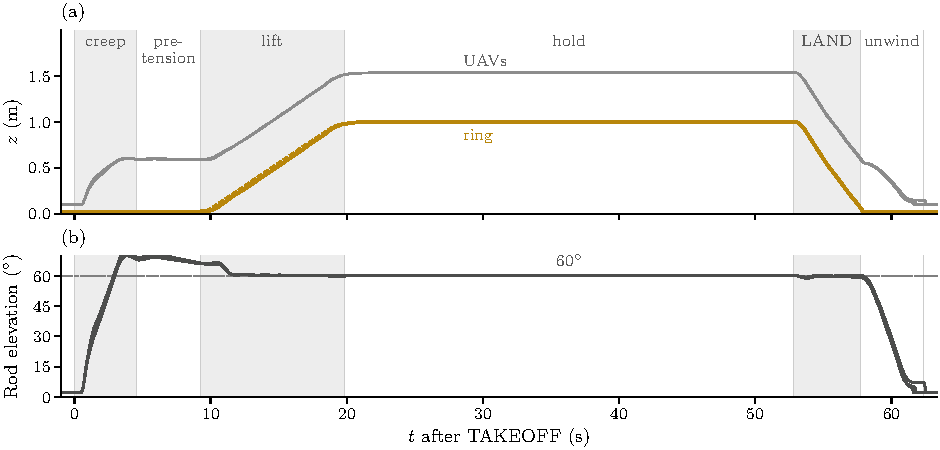
\includegraphics[width=\textwidth]{Images/flight.pdf}
\caption[One flight from the floor]{One flight from the floor in the rig twin: three carriers, hover at 1.0\,m, the
default controller (their traces overlap). (a) Heights of the ring (gold; dashed: its planned height) and of the
UAVs (grey); shaded: the creep, the lift and LAND. (b) Elevation of each rod above the horizontal; dotted: the
planned 60$^\circ$. In the creep the UAVs climb and swing their rods up from the floor, past the planned elevation,
without lifting the ring; in the pretension they hold their height while the rod feedforward eases in; the ring
then leaves the floor and follows its lift ramp to 1.0\,m while the rods settle on 60$^\circ$. On LAND the ring and
the UAVs descend together until the ring is on the floor; the UAVs then unwind along their rods.}
\label{fig:flight}
\end{figure}

\subsubsection{The carry in the twin: a speed envelope}
\label{sec:res_envelope}

Table~\ref{tab:T7t} gives the three-carrier carry in the rig twin: five load paths at three peak path speeds, two
runs per cell on one code tree, and an arm with 1\,m cables, scored against four bars frozen before the runs: no
abort, drop or unannounced detach, with every UAV landed and disarmed; a ring RMSE of at most 25\,mm (from 5\,s after TAKEOFF to LAND, lift and landing included); a peak ring
tilt of at most 6$^\circ$; and a radius ratio of at least 0.95. 39 of the 40 runs pass every bar. The spin at
0.3\,m/s fails the tilt bar once (6.31$^\circ$, mid-spin; its repeat 3.76$^\circ$), so as frozen that cell is outside
the envelope, and it was not re-flown; every other cell is inside at 0.125, 0.2 and 0.3\,m/s. The radius ratio lies
between 0.966 and 1.004 over all 40 runs (for the line, the ratio of amplitudes about its centre). The 1\,m cables
pass every bar, with a ring RMSE at most 1.27 times their 0.55\,m cell's mean on the frozen window (1.35 times on the
path alone); their configurations also land 5\,s later, so the comparison is not one variable.

\begin{table}[htbp]
\centering
\footnotesize
\setlength{\tabcolsep}{2.6pt}
\caption[The carry in the twin: the speed envelope]{The three-carrier carry in the rig twin: 0.86\,kg ring at
1.0\,m on 0.55\,m rods (lower block: 1\,m cables), floor start, the default controller, two runs per cell on one
code tree; each cell gives the range over its two runs. Scored against the bars frozen before the runs: the ring RMSE
from 5\,s after TAKEOFF to LAND, lift-off, hovers and descent included, against the planner's 10\,Hz held reference
(bar 25\,mm), and the peak ring tilt over the whole flight, lift-off and landing included (bar 6$^\circ$). Reported
beside them, not scored: the same RMSE and the peak tilt over the path alone, and the clock-free measures of
Section~\ref{sec:metrics}: the cut (mean distance inside the path over its tightest quarter), the across-path rms over
the fast part of the path, and the lag behind the schedule (+ late). Speed: the peak path speed. $^a$\,One run over the
tilt bar: the cell is outside the envelope. Line: no curvature, so no cut; its lag is not defined at the turns and is
not given.}
\label{tab:T7t}
\begin{tabular}{llccccccc}
\toprule
 & & \multicolumn{2}{c}{Scored} & \multicolumn{5}{c}{Reported} \\
\cmidrule(lr){3-4}\cmidrule(lr){5-9}
 & Speed & Ring RMSE & Peak tilt & Path RMSE & Path tilt & Cut & Across rms & Lag \\
Path & (m/s) & (mm) & ($^\circ$) & (mm) & ($^\circ$) & (mm) & (mm) & (ms) \\
\midrule
Circle & 0.125 & 8.8--10.6 & 1.8--1.9 & 4.3 & 0.9--1.1 & 2.4--2.5 & 2.7--2.8 & 55--70 \\
 & 0.2 & 9.2--12.4 & 1.7 & 6.2--8.9 & 1.4--1.6 & 3.4--6.6 & 4.4--8.3 & 32--73 \\
 & 0.3 & 14.0--14.7 & 2.0--2.8 & 13.4--14.3 & 2.0--2.8 & 13.0--14.3 & 14.6--15.8 & 54--56 \\
\addlinespace
Figure-eight & 0.125 & 10.3--12.7 & 2.3 & 6.0--8.9 & 1.0--1.1 & 4.9--10.0 & 3.5--7.1 & 34--63 \\
 & 0.2 & 13.6--14.5 & 1.9--2.0 & 11.9--12.4 & 1.5--1.7 & 15.8--16.0 & 10.2--10.9 & 36--44 \\
 & 0.3 & 17.8--17.9 & 2.3--2.4 & 20.2--20.9 & 2.3 & 28.5--31.1 & 17.9--20.6 & 15--25 \\
\addlinespace
Line & 0.125 & 6.5--8.3 & 1.9--2.0 & 4.3--5.3 & 0.9--1.0 & -- & 0.4--0.5 & -- \\
 & 0.2 & 9.1--9.8 & 2.5--2.8 & 8.3--9.0 & 1.5--1.9 & -- & 0.5--1.1 & -- \\
 & 0.3 & 12.5--16.8 & 3.0--3.7 & 12.9--16.9 & 2.4--3.0 & -- & 0.5--1.0 & -- \\
\addlinespace
Orbit & 0.125 & 8.1--10.1 & 1.8--1.9 & 6.7--8.7 & 1.0--1.1 & 3.6--4.7 & 3.9--5.1 & 72--90 \\
 & 0.2 & 12.0--13.7 & 2.0--2.3 & 11.6--12.7 & 1.7--1.9 & 8.5--9.5 & 8.9--10.0 & 57--63 \\
 & 0.3 & 17.1--17.8 & 2.8--2.9 & 18.3--19.3 & 2.5--2.8 & 11.6--12.7 & 13.2--15.2 & 27--34 \\
\addlinespace
Spin & 0.125 & 10.4--10.5 & 1.9 & 5.6--5.7 & 1.0--1.1 & 1.5--3.3 & 2.5--4.4 & 78--87 \\
 & 0.2 & 11.3--11.5 & 2.0--2.2 & 6.2--8.5 & 1.9--2.2 & 0.4--5.8 & 3.2--7.4 & 45--60 \\
 & 0.3 & 14.2--15.9 & 3.8--6.3$^a$ & 13.5--18.5 & 3.8--6.3 & $-$6.3 to $-$1.2 & 11.4--13.7 & $-$3 to 39 \\
\midrule
\multicolumn{9}{l}{\emph{1\,m cables}} \\
Circle & 0.125 & 10.3--11.1 & 1.8 & 4.8--5.8 & 0.9--1.0 & 2.3--3.3 & 2.9--3.9 & 63--82 \\
Circle & 0.2 & 12.1--12.4 & 1.8--2.0 & 9.3--9.4 & 1.4--1.7 & 6.8--7.7 & 9.4--9.6 & 72--77 \\
Figure-eight & 0.2 & 14.6--16.0 & 1.7--2.5 & 14.3--15.7 & 1.7--2.3 & 20.4--20.6 & 13.1--14.7 & 36--56 \\
Line & 0.2 & 11.0--12.0 & 1.9--3.0 & 9.6--11.2 & 1.6--3.0 & -- & 1.2 & -- \\
Orbit & 0.2 & 11.9--13.2 & 2.2--2.8 & 11.5--12.6 & 1.8 & 8.2--9.5 & 8.4--9.8 & 48--60 \\
\bottomrule
\end{tabular}
\end{table}
% Runs (registry): circle R1847/R1848, R1857/R1858, R1859/R1860; fig-8 R1849/R1850, R1861/R1862, R1863/R1864;
% line R1851/R1852, R1865/R1866, R1867/R1868; orbit R1853/R1854, R1869/R1870, R1871/R1872; spin R1855/R1856,
% R1873/R1874, R1875/R1876; L100 R1877-R1886. Tree: week5 4b3560e flight code (lab PC), read-back identical in all 40.

On the clock-free measures the ring runs slightly inside its curves, by more as speed rises, and up to 0.09\,s
behind its schedule (Table~\ref{tab:T7t}): at 0.3\,m/s it sits 28--31\,mm inside the figure-eight's tight bends and
12--14\,mm inside the circle and the orbit, against about 2--10\,mm at 0.125\,m/s. Where along the cascade the cut appears was traced in an exploratory study: the UAVs fly their
references to within 0.5\,mm across the path, and the planner's own plan half a second ahead is already as far
inside as the ring ends up, so the cut is in the plan. Shifting the trackers' references in time removed it on the
circle and the orbit, but the shift that centred them failed its neighbour check on the spin, and the test of whether
the shift stands for the loop's delay failed, so the cut's source is open; the defaults stay and the lag is reported
(Appendix~\ref{sec:app_corner}). Figure~\ref{fig:traj} shows the ring's path at the rig's speed.

\begin{figure}[htbp]
\centering
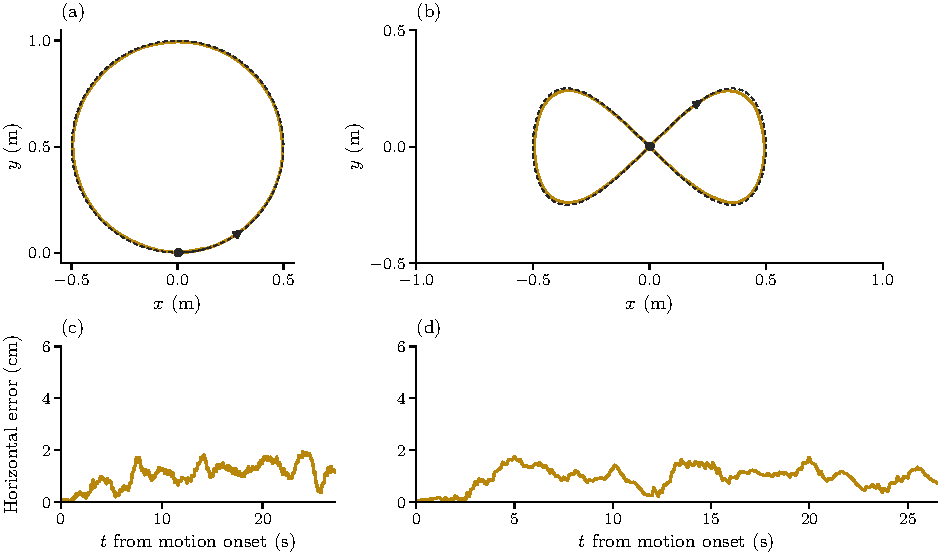
\includegraphics[width=\textwidth]{Images/trajectories.pdf}
\caption[The ring's path in the twin]{The ring's path in the rig twin at the rig's speed: three carriers, 0.125\,m/s
peak path speed, one run of each from the carry claim. (a) The orbit, one lap of radius 0.5\,m; (b) the figure-eight,
$a = 0.5$\,m. Gold: the ring's centre; dashed: the path; dot and arrow: start and direction. (c, d) The ring's
horizontal distance from the planner's reference, sampled at its 10\,Hz updates, from the onset of motion; this
time-indexed error includes the lag, which Table~\ref{tab:T7t} reports apart.}
\label{fig:traj}
\end{figure}

\subsubsection{The carry on the rig}
\label{sec:rig_results}

The hardware campaign covers carrying the ring with three and four UAVs and, since 7 October, releasing one UAV in
flight (Section~\ref{sec:res_leave}); the attach has not yet completed on the rig (Section~\ref{sec:res_join}). The
rig days, and what each changed, are in Appendix~\ref{sec:app_rig}. On 7 October four UAVs carried the ring on the
circle and the figure-eight, first on the planned rod pull and then with the trackers' measured pull and the rods
planned at 60$^\circ$ (Section~\ref{sec:tracker}; Table~\ref{tab:T7} and Figure~\ref{fig:F8}). Both paths flew about
three times closer to their references, the lags fell by half to two thirds, and the height's standard deviation fell from about 5 to
0.5\,cm. Six settings changed at once (Table~\ref{tab:T7}), so the table shows their combined effect: the measured pull alone flew the rods
at the planned 45$^\circ$, where a magnet let go 3.9\,s into the circle, and planning 60$^\circ$ keeps each magnet's
pull closer to its axis.

\begin{table}[htbp]
  \centering
  \footnotesize
  \caption[The carry on the rig]{The carry on the rig: four UAVs, the 0.86\,kg ring at 1.0\,m; the pull source and the
  rod plan against the path error. Error: the ring centre's horizontal distance from its reference from 4\,s into the
  path to LAND, mean and largest; lag: the time shift of the reference that minimises that error; height sd over the
  same window; one run each. K1 against K2 and K5 against K6 differ in six settings (pull source, planned and
  hand-over elevation, the pull cap, the landing unwind, the delay compensation): two configurations, not the pull
  source alone. [K3, K4 and K7: the next rig day.]}
  \label{tab:T7}
  \begin{tabularx}{\textwidth}{lYccYccc}
    \toprule
    Flight & Path & Pull source & Rod plan & Error mean / max (cm) & Lag (s) & Height sd (cm) & $n$ \\
    \midrule
    K1 & circle 0.125\,m/s & planned & 45$^\circ$ & 7.9 / 16.9 & 0.47 & 4.9 & 1 \\ % r006 (7 Oct); reviewer 12 Oct recomputed on this window; the registry row read 8.25 / 0.45 / 4.8 on the card's script
    K2 & circle 0.125\,m/s & measured & 60$^\circ$ & 2.6 / 5.5 & 0.17 & 0.5 & 1 \\ % r206e60; the registry's 2.91 / 0.20 are >10 % off on this window (reviewer): the R3 falsifier stays frozen on 2.91
    K3 & circle 0.125\,m/s & measured & 60$^\circ$ & [\dots] & [\dots] & [\dots] & [\dots] \\ % the repeat
    K4 & circle 0.125\,m/s & planned & 60$^\circ$ & [\dots] & [\dots] & [\dots] & [\dots] \\ % the falsifier
    K5 & figure-eight 0.25\,m/s & planned & 45$^\circ$ & 8.2 / 19.9 & 0.37 & 4.8 & 1 \\ % r0007; the registry's 0.41 s was a best shift too, its own row says 0.65 (along-track over speed)
    K6 & figure-eight 0.25\,m/s & measured & 60$^\circ$ & 2.9 / 6.6 & 0.19 & 0.6 & 1 \\ % r2008e60; registry 3.0 / 0.21 / 0.6
    K7 & hover 3 min & measured & 60$^\circ$ & [\dots] & -- & [\dots] & 1 \\ % the long hover
    \bottomrule
  \end{tabularx}
\end{table}

\begin{figure}[htbp]
\centering
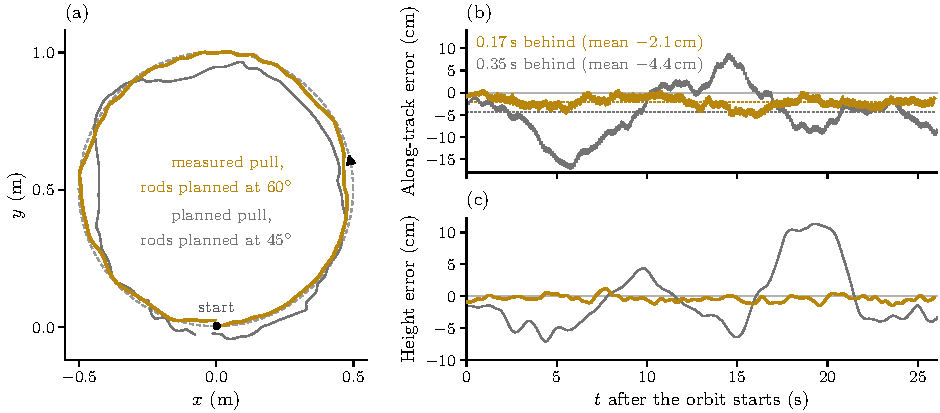
\includegraphics[width=\textwidth]{Images/rig_carry.pdf}
\caption[The circle on the rig: measured pull against planned pull]{The four-UAV circle on the rig, radius 0.5\,m at
0.125\,m/s, one lap: the trackers fed the rod pull they measure from motion capture with the rods planned at
60$^\circ$ (gold), against the same circle flown that morning on the planner's pull with the rods planned at
45$^\circ$ (grey); one run each. (a) Plan view of the ring's centre against the reference circle (dotted), with the
start and the direction of travel. (b) Along-track error, the ring's position along the circle minus the
reference's, negative behind; dotted: each run's mean, 2.1\,cm (0.17\,s) and 4.4\,cm (0.35\,s) behind, with the
worst 5.5 and 17\,cm. (c) Height error, measured minus planned, with a standard deviation of 0.5\,cm against
5.0\,cm.}
\label{fig:F8}
\end{figure}

\paragraph{The 60$^\circ$ planned-pull circle.} [Frozen falsifier, to score after the rig flies K4: if K4 lies within
max(1\,cm, the lap-to-lap sd of K3) of 2.91\,cm, the gain came from the rod angle, not the measurement. The 2.91\,cm
was frozen from the 7 October card's reading of K2; on this table's window the same flight reads 2.6\,cm, a
difference inside the 1\,cm tolerance.] In the twin (the even ring, two runs each, 0.09\,cm over the frozen floor) the planned
pull tracked the 60$^\circ$ circle better than the measured pull (Section~\ref{sec:res_levers}), so the twin does not
explain the rig's gain.
% 12 Oct: K1, K2, K5, K6 recomputed by the reviewer on one definition (window +4 s to LAND, lag by best time shift);
% the first-lap along-track numbers of fig:F8 (2.1 / 4.4 cm, 0.17 / 0.35 s) are a different window and are not these.

\subsubsection{Thrust identification}
\label{sec:thrust_id}

The 13 free hovers of Section~\ref{sec:tracker} fit
\begin{equation}
    u_T = a_i + 0.507\,M - 0.022\,(V - 23.5),
    \label{eq:thrust_fit}
\end{equation}
with $u_T$ the throttle, $M$ the mass carried (kg), $V$ the battery voltage and offsets $a_i$ of
0.181--0.187 for the four UAVs, with an rms residual of 0.003 (Figure~\ref{fig:thrust_map}). Above its
offset the map has a gain of 35.2\,m/s$^2$ per unit throttle for a 0.55\,kg UAV, which is the $k_T$ of
the tracker model \eqref{eq:trk_model}. With the map and one shared offset, the four UAVs hovered free
at +3.7, $-0.5$, $-0.4$ and +0.9\,cm from their targets with no integral action; the one 3.7\,cm high is
the UAV whose own offset is the lowest. A map identified at hover with one proportional gain had left
the UAVs 14--17\,cm low. Carrying the ring, the throttle the UAVs needed (0.55--0.60) matched what the
map predicted for their share of the load (0.569--0.575).

\begin{figure}[htbp]
\centering
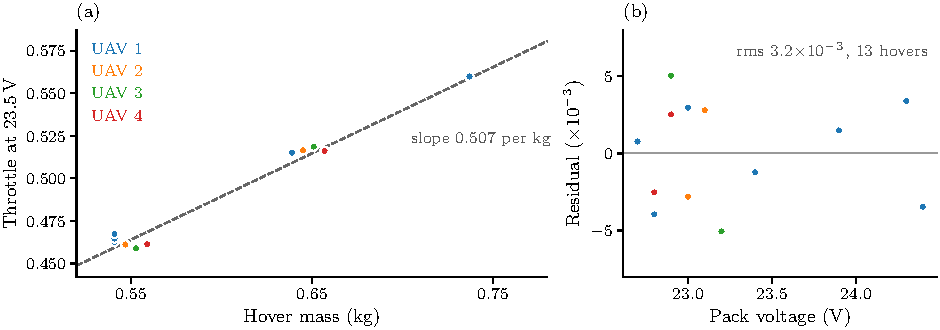
\includegraphics[width=\textwidth]{Images/thrust_map.pdf}
\caption[The rig's thrust map]{The rig's thrust map from 13 free hovers on 30 September, each UAV carrying 0, 98 or
196\,g. (a) Hover throttle corrected to 23.5\,V and to the mean offset, against the hover mass; one colour per UAV
(markers offset sideways by up to 9\,g so that hovers at the same mass can be seen); dashed: the fit
\eqref{eq:thrust_fit} with per-UAV offsets $a_i$ of 0.181--0.187. (b) The residuals of the fit against the pack
voltage: rms $3.2\times10^{-3}$, at most $5\times10^{-3}$ (about 1\,\% of hover throttle), with no trend left in
voltage.}
\label{fig:thrust_map}
\end{figure}

\subsubsection{Landing}
\label{sec:sim_landing}

Over the 82 landings of the freeze code tree in the rig twin (Table~\ref{tab:land}, Appendix~\ref{sec:app_tests}),
the unwind, the feedforward ramp and the ground idle kept every UAV within 0.65\,cm outside its reference and its lean
1.2\,s after touchdown at most 4.7$^\circ$ up to the moment the fleet was declared landed, where a straight descent pushed the UAVs 23.5\,cm outward. But 4 of the
82 landings disarmed the fleet with the UAVs still in the air, all four with one UAV stronger than its thrust map:
in three, every UAV was 0.46--0.53\,m up and fell onto its side. The stall test that declares touchdown had used up
its grace in the loaded descent, and when the ring touched down the strong UAV nearly held its height through the
second in which the UAVs blend to free hover, which read as a stall. With correct thrust maps on the rig's own
landing path (no unwind) the same fire came in 2 of 4 twin runs, at 0.42\,m. Re-arming the stall test at ring
touchdown (Section~\ref{sec:takeoff}) removed it in all 5 runs on that path and is now the twin's default; the rig
gets it after a review of its pose-freshness check. A UAV whose throttle offset is 0.03 below its map's (about 1\,m/s$^2$ of surplus thrust)
still stops about 16\,cm above its rest once the ring is down, is disarmed there and leans onto its rigid rod (Section~\ref{sec:discussion}); a
descent that keeps lowering its target for that case is under test.
% Sources: appendix re-fly (R2032, R2044, R2045 at 0.46-0.53 m; R2033 0.26 m; reviewer 17 Oct 02:40, C-L1 NOT
% supported); touchdown card re-fly (rig LAND path off 2 of 4: R2094, R2135; A 0 of 5: R2095, R2106, R2134, R2136,
% R2137; reviewer supported, twin default; must not say "ready for the rig"); residual 15.7-15.8 cm, 23.6-29.9 deg
% (R2088-R2091, R2099-R2102); land_descend_to_stall rev 3 flying 17-18 Oct (not thesis evidence yet).

\subsubsection{Computation}
\label{sec:res_compute}

Figure~\ref{fig:solve_time} gives the planner's optimisation time per tick in flight on the rig, 7--8
October, on the laptop that also runs the motion-capture and radio nodes. No tick of 7--8 October reached the 100\,ms tick. On
the rig days of 14--15 October, with three UAVs and the collaborator's stack running beside it, the planner solved in
31--46\,ms at the median and 46--65\,ms at the 95th percentile, with a slowest tick of 67--116\,ms. [The four-UAV median of 51--66\,ms against the rig's
60\,ms solve budget: to explain from the logs.] In the twin the stack solves 2--4 times slower than the solver alone,
under the load of the physics and the other nodes, but simulated time waits for the planner, so it always meets its
tick there. The 25 solve failures of the last rig flight of 30 September were traced to two faults acting together,
both now guarded (Appendix~\ref{sec:app_rig}).

\begin{figure}[htbp]
\centering
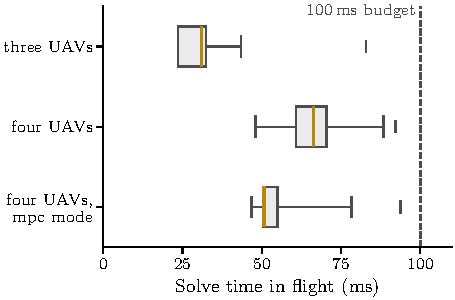
\includegraphics{Images/solve_time.pdf}
\caption[Planner solve time on the rig]{The planner's optimisation time in flight on the rig, 7--8 October:
three UAVs (after a detach, 15\,883 ticks), four UAVs (detach mode, 4\,762 ticks; carry mode, 22\,385 ticks). Box:
quartiles and median (gold); whiskers: 1st and 99th percentile; bar: the slowest tick. Medians 31, 66 and 51\,ms;
99th percentiles 44, 88 and 78\,ms; no tick reached the 100\,ms tick (dashed).}
\label{fig:solve_time}
\end{figure}

\paragraph{Answer to RQ1, the carry.} Yes, at lab speeds. On the rig four UAVs carried the ring around the circle
and through the figure-eight within 3\,cm of the path on average with the measured rod pull and the rods planned at
60$^\circ$, against about 8\,cm before (six settings changed together, so the measured pull alone is not yet
isolated); in the twin three UAVs carried it on five paths at peak path speeds up to 0.3\,m/s inside the frozen bars,
except the spin at 0.3\,m/s, and on 1\,m cables in the five cells flown up to 0.2\,m/s, with the ring running further
inside its curves as speed rises. A landing can still disarm a UAV in the air when its thrust
map is wrong: the re-armed touchdown test removes the 0.4--0.5\,m case in the twin, not the 16\,cm one, and the rig
does not have it yet.


% res_steady.tex -- Results 4.1 (cont.): the steady payload error, rig and twin.
% 17 Oct (v3_full): rewritten around the measured rod pull after the appendix re-fly on the freeze tree
% (docs/analysis/appendix_refly_2026-10-17.md: C-X1, C-X2, C-D1, C-D4, C-R1-R4 confirmed; C-D2, C-D3, C-D5 falsified;
% C-G1, C-G2 unresolved; the reviewer's must-not-say list honoured: no 8.4 cm, no "learns the push" vertically, no
% 0.76 N as learned, no geometric explanation of +17.1 cm, the +13 cm box offset is not a tracking error, no "the model
% integral fails on the thrust-map error", the mass result always with the measured pull and the rigid-rod twin) and
% the exploratory cable_source model pair (R2084-R2087: push -7.95 cm, +20 % mass +22.2 cm). Rig sources unchanged:
% registry RIG-1001-*, RIG-1007-r0001/r002/r20004 (fig:rig_integral), docs/rig_2026-09-30_review.md.

\subsubsection{Steady payload error}
\label{sec:res_steady}

This part of RQ1 asks what leaves a steady error in the payload's position, and what removes it. Each source is
set against the same flight without its remedy, its baseline; the bar is the ring back within 1\,cm of its target.
On the rig, the measured rod pull is what changed the picture, and it does the same in the twin.

\paragraph{On the rig: the model integral and the measured rod pull}
\label{sec:res_rig_integral}
% Rig 7 Oct: RIG-1007-r0001 (no integral), r002 (model integral, planned pull), r20004 (model integral +
% measured pull); planner log.csv; figure tools/thesis_rig_figures.py rig_integral.

On 7 October the rig flew three hovers at 1.0\,m with four UAVs, changing one thing at a time
(Figure~\ref{fig:rig_integral}). Without an integral the ring sank in the 5\,s it held before LAND. The model
integral brought it back to its target by learning a downward force of up to 0.9\,N, but the ring then bobbed
at about 0.2\,Hz. With the trackers' measured rod pull added (Section~\ref{sec:tracker}) it held within 2\,cm
and the integral learned only 0.1\,N: most of the missing force was in the rods' pull, which the planned pull
got wrong. On the circle and the figure-eight, the measured pull with the rods planned at 60$^\circ$ cut the
standard deviation of the ring's height from 4.8--4.9 to 0.5--0.6\,cm (Table~\ref{tab:T7}). Each is one run; the
measured-pull hover held for 7\,s, ending before the first swing of the integral-only run, so the circle and the
figure-eight, flown for 36 and 68\,s, carry the claim that the swing is gone.

\begin{figure}[htbp]
\centering
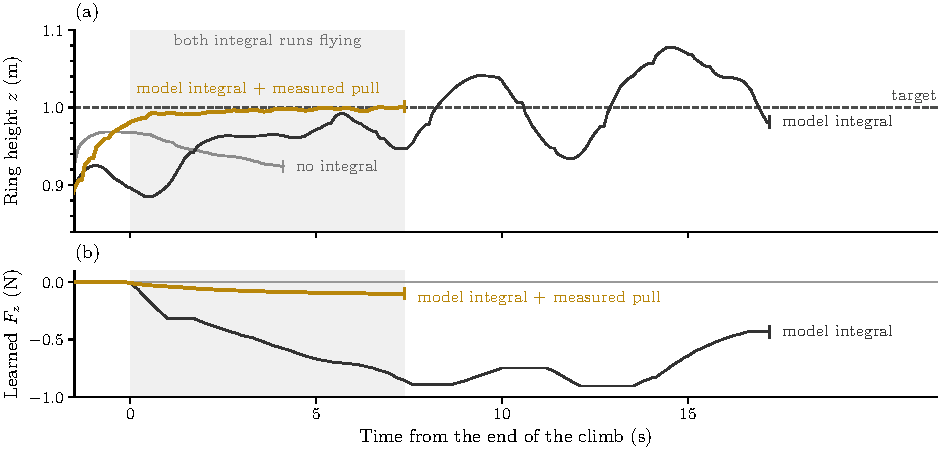
\includegraphics[width=\textwidth]{Images/rig_integral.pdf}
\caption[The model integral and the measured pull on the rig]{Ring height on the rig in a hover at 1.0\,m with
four UAVs, one change at a time (7 October, one run each; each trace ends at LAND, marked by a tick; shaded: the
7\,s both integral runs flew). (a) Without an integral the ring sank from 0.97 to 0.92\,m. With the model integral
it dipped to 0.89\,m after the climb, came back up, and from 8\,s bobbed between 0.93 and 1.08\,m at about
0.2\,Hz. With the integral and the trackers using the measured rod pull it held between 0.98 and 1.00\,m.
(b) The vertical force the model integral learned (negative: downward, a force the model lacked): up to
$-0.9$\,N with the planned pull, $-0.1$\,N with the measured one. The flat stretches are the integral frozen by
design while the ring moves faster than 0.05\,m/s vertically.}
\label{fig:rig_integral}
\end{figure}

\paragraph{External forces}
\label{sec:res_force}

In the twin a constant force was applied to the hovering ring for 15\,s: 0.6\,N downward, about the weight of a
60\,g object, and 0.4\,N horizontally (Table~\ref{tab:disturbance}). The two axes now behave differently. The
vertical push leaves no steady offset, with or without an integral: each tracker's measured pull takes up its share
within about a second, so the ring dips 1.4\,cm and is back within 1\,cm 1.0--1.1\,s after the onset, and the
integral is left with nothing to remove. An exploratory pair with the trackers on the planner's pull instead, and
nothing else changed, left the ring 8.0\,cm low under the same push, which places the effect in the measured pull.
Horizontally the measured pull does not act on the ring's position, and the push leaves the ring 4.8\,cm off its
target; the model integral removes that offset, its force settling at 0.32\,N against the 0.40\,N applied
(Figure~\ref{fig:disturbance}). It does so as integral action does: the peak is barely reduced, because the integral
($1/k_i = 2.5$\,s) is slower than the cascade, and when the push ends the integral still holds its force and drives
the ring past the target by about as much as the push displaced it at onset (5.3\,cm). Doubling $k_i$, or keeping
the integral's speed gate only for the first 5\,s after the lift, made no difference the resolution rule could
resolve on the vertical push (Table~\ref{tab:gain}, Appendix~\ref{sec:app_tests}); there the integral barely moves.
When one UAV produces more thrust than its map assumes, neither form of the integral leaves a height or horizontal
error, and the ring hovers level (0.1$^\circ$); the trace reads as that UAV's own measured pull taking up its error,
which a force on the payload could not represent, though no one-variable pair separates it.

\begin{figure}[htbp]
\centering
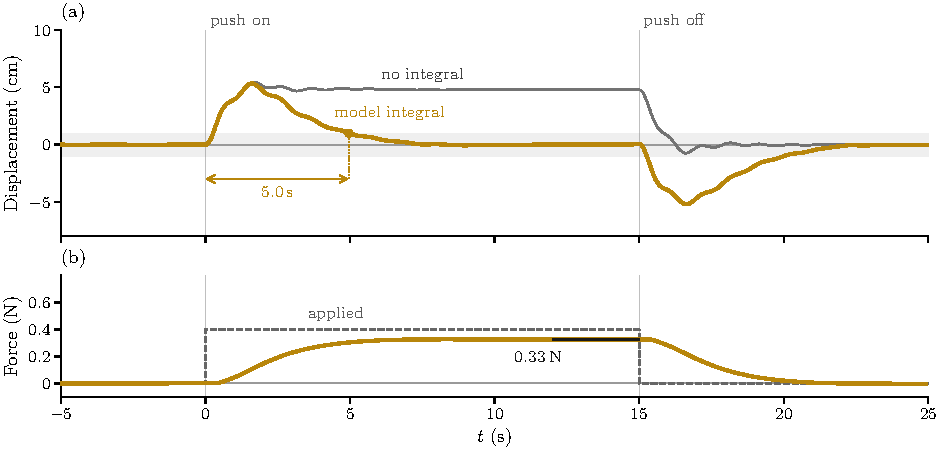
\includegraphics[width=\textwidth]{Images/disturbance.pdf}
\caption[Rejection of a horizontal force on the ring]{Rejection of a constant horizontal force on the ring in the
rig twin: three carriers, hover at 1.0\,m, the measured rod pull; a 0.4\,N push acts from 0 to 15\,s; one run of
each case (Table~\ref{tab:disturbance} gives both runs and the vertical push). (a) Ring displacement along the push,
relative to its mean over the 5\,s before: no integral (grey) and the integral in the planner's model (gold). Band:
$\pm 1$\,cm. Arrow: the time for the model integral to bring the ring back within 1\,cm for good. (b) Change of the
model integral's force $\mathbf{d}$ along the push from its value before the push (gold), against the applied force
(dashed). Black bar: its mean over the last 3\,s of the push.}
\label{fig:disturbance}
\end{figure}

\begin{table}[htbp]
\centering
\caption[Disturbance rejection in the twin]{Disturbance rejection in the rig twin: three carriers in hover at 1.0\,m,
$\epsilon = 0$, two runs per cell on the freeze code tree. Displacement along the force, relative to its mean over
the 5\,s before the push; time to within 1\,cm after the onset; the change of the integral's force from its value
before the push.}
\label{tab:disturbance}
% generated by tools/thesis_sim_tables.py on the freeze tree (17 Oct; appendix re-fly R2027-R2033, R2039-R2045), then
% edited by hand: the planned-pull column (exploratory pair R2084, R2086, cable_source model) and footnotes a-c from
% the reviewer's corrections (docs/analysis/appendix_refly_2026-10-17.md).
\footnotesize
\setlength{\tabcolsep}{4pt}
\begin{tabular}{lcccc}
\toprule
 & \multicolumn{3}{c}{Measured rod pull} & Planned pull \\
\cmidrule(lr){2-4}\cmidrule(lr){5-5}
 & No integral & Target shift & Model integral & No integral$^c$ \\
\midrule
\multicolumn{5}{l}{\emph{0.6\,N downward push on the ring}} \\
\quad steady displacement (cm) & 0.0 (2) & 0.0 (2) & 0.0 (2) & 8.0 (2) \\
\quad peak displacement (cm) & 1.4 (2) & 1.3 (2) & 1.3 (2) & -- \\
\quad overshoot after release (cm) & 1.4 (2) & 1.5 (2) & 1.4 (2) & -- \\
\quad time to within 1\,cm (s) & 1.1 (2) & 1.0 (2) & 1.1 (2) & -- \\
\quad change of the integral force (N) & -- & -- & 0.10$^a$ (2) & -- \\
\midrule
\multicolumn{5}{l}{\emph{0.4\,N horizontal push on the ring}} \\
\quad steady displacement (cm) & 4.8 (2) & n/a & 0.0 (2) & -- \\
\quad peak displacement (cm) & 5.4 (2) & n/a & 5.5 (2) & -- \\
\quad overshoot after release (cm) & 0.7 (2) & n/a & 5.3 (2) & -- \\
\quad time to within 1\,cm (s) & -- & n/a & 4.9 (2) & -- \\
\quad change of the integral force (N) & -- & n/a & 0.32 (2) & -- \\
\midrule
\multicolumn{5}{l}{\emph{One UAV producing more thrust than its map assumes$^b$}} \\
\quad height error (cm) & -- & 0.0 (2) & $-$0.1 (2) & -- \\
\quad horizontal error (cm) & -- & 0.0 (2) & 0.0 (2) & -- \\
\quad ring tilt (\si{\degree}) & -- & 0.1 (2) & 0.1 (2) & -- \\
\bottomrule
\multicolumn{5}{p{0.95\textwidth}}{\footnotesize $^a$\,Not a learned force: it doubles with the integral gain
(0.21--0.22\,N at $k_i = 0.8$) and drifts by $-0.05$\,N with no push; the measured pull has already taken the push
up. $^b$\,Its real throttle offset 0.03 below the 0.185 its tracker assumes. $^c$\,Exploratory pair: the trackers on
the planner's pull, everything else as the first column, flown on a later code tree whose flight code differs only by
switches that are off.}
\end{tabular}

\end{table}

\paragraph{Wrong model values}
\label{sec:sim_robustness}

The controller is given the payload's mass, the rod lengths, the attachment radius and each UAV's thrust map; on the
rig each is measured, and each can be wrong. In the twin's hover with one wrong value in the controller while the
simulated rig keeps the true ones (Table~\ref{tab:robust}, Appendix~\ref{sec:app_robust}), a payload mass typed
20\,\% high or low leaves the hover where it was, with or without the integral, because the measured pull at each UAV
carries what the ring actually weighs; in an exploratory pair on the planner's pull the same $+20$\,\% error left the
ring 22.2\,cm high. That is a result of the rigid-rod twin on the measured pull, not a licence to type the mass
loosely. Rods typed 5\,cm long are absorbed when they are measured at the hand-over; unmeasured, they leave the ring
17.1\,cm high with or without the integral, whose tautness gate stays closed because the rods read as partly slack.
An attachment radius typed 2\,cm large leaves the ring 0.9\,cm high, and the vertical integral winds up through the
hold without moving it, to 0.76\,N by LAND: not a learned force, and a reason the integral's bound and its warning
matter. All 28 flights landed, and the ring's tilt stayed at 0.1$^\circ$.

\paragraph{The tracker's initial condition}
\label{sec:res_ic}

An earlier version of the tracker relaxed its initial condition to a box with $\epsilon = 0.025$
(Section~\ref{sec:tracker}). On the freeze tree the box holds the ring 13.1\,cm above its target in hover and
13.0\,cm on the orbit, where pinning node~0 to the measurement holds it within 0.1\,cm, and pinning also cuts the
orbit's horizontal error from 3.9 to 0.7\,cm (Table~\ref{tab:x0}, Appendix~\ref{sec:app_tests}). The offset is not
a tracking error of the UAVs: the references the planner sends them are themselves 10.6\,cm higher. It is a bias in
the cascade, not a force, which is why no force estimate of the earlier stack could find it.

\paragraph{The breakaway cap}
\label{sec:res_cap}

On the rig on 1 October (Table~\ref{tab:rig_oct1}, Appendix~\ref{sec:app_rig}), without the height integral the ring
held 5\,cm low at 0.5\,m, and at higher targets it sat 20--30\,cm low before the integral took over, which then
saturated at its bound. The cause was found afterwards in the logs: the breakaway freeze of
Section~\ref{sec:takeoff} had held the pull at the fraction reached at breakaway for the whole flight, so the trackers
were told the rods pull 7--27\,\% less than they do. Holding the pull at 75\,\% in the twin reproduced the rig's
height shortfall and its steeper rods. The cap has been released once the lift starts since 7 October.

\paragraph{The rig's pull towards $-x$.} In every rig flight of 1 October the ring sat 3--17\,cm from its horizontal
reference, always towards the room's $-x$ direction, and nothing in the controller then pulled it back. The offset
kept its direction when the whole system was rotated by 124$^\circ$, so it does not come from a particular UAV, rod
or the ring. Estimated offline from the UAVs' delivered thrust less the total weight, the force behind it was
0.41--0.52\,N towards $-x$, about 1$^\circ$ of the fleet's thrust; moving the system 1.1\,m towards $+x$ reduced the
offset to 3--5\,cm, in a single flight. A motion-capture ground plane tilted by about 1$^\circ$, or air moving in
the room, remain the two explanations; the model integral, which removes a horizontal force in the twin, has flown on
the rig since 7 October.

\paragraph{Tilt and height.} On the rig the ring's mean tilt fell from 5.0$^\circ$ at 0.45\,m to 1.6$^\circ$ at
0.94\,m (1 October): close to the floor the ring sits in the UAVs' downwash and its recirculation, and flying higher
was the most effective single change for a steady ring.

\paragraph{Sources of steady error}

Table~\ref{tab:error_sources} collects the sources found, how each shows at the payload and what removes it. The
approaches to model error flown on the earlier stack (a force balance, an offset-free observer, the measured cable
force, a thrust-gain trim, the rods' mass in the planner) are recorded in Appendix~\ref{sec:app_methods}; the measured
cable force is the one that became the default.

\begin{table}[htbp]
\centering
\footnotesize
\caption{Sources of steady payload error found in this work, how each shows at the payload and what
removes it, on the current controller.}
\label{tab:error_sources}
\begin{tabularx}{\textwidth}{>{\raggedright\arraybackslash}p{3.2cm}>{\raggedright\arraybackslash}X>{\raggedright\arraybackslash}Xl}
\toprule
Source & Signature at the payload & Remedy & Section \\
\midrule
Tracker's relaxed initial condition & held high in hover and on the orbit (13\,cm in the twin); in the
references, not a tracking error; not a force & pin node~0 to the measurement & \ref{sec:res_ic} \\ \addlinespace
Breakaway cap held for the whole flight & held low; rods steeper than planned (rig) & release the cap once
the lift starts & \ref{sec:res_cap} \\ \addlinespace
A vertical force on the ring & none on the measured pull; on the planned pull a steady drop (8\,cm for 0.6\,N,
exploratory) & the measured rod pull at each UAV & \ref{sec:res_force} \\ \addlinespace
A horizontal force (a push, wind, the rig's pull towards $-x$) & steady displacement along the force (4.8\,cm for
0.4\,N in the twin) & the model integral & \ref{sec:res_force} \\ \addlinespace
Payload mass typed wrong & none on the measured pull in the rigid-rod twin; on the planned pull a height offset
(22\,cm for $+20$\,\%, exploratory) & the measured rod pull & \ref{sec:sim_robustness} \\ \addlinespace
Rods typed long, not measured & held high (17\,cm for $+5$\,cm); the rods read partly slack, so the integral's gate
stays closed & measure the rods at the hand-over & \ref{sec:sim_robustness} \\ \addlinespace
Attachment radius typed wrong & held 0.9\,cm high for $+2$\,cm; the vertical integral winds up without effect &
none yet: the radius is measured on the rig & \ref{sec:sim_robustness} \\ \addlinespace
One UAV's thrust map wrong & none in hover on the measured pull; a tilt and a horizontal offset on the planned
pull (earlier stack) & that UAV's own measured pull & \ref{sec:res_force} \\
\bottomrule
\end{tabularx}
\end{table}

\paragraph{Answer to RQ1, steady errors.} The measured rod pull, not the integral, is what holds the ring's height on
this controller: in the rigid-rod twin it takes up a vertical push and an error in the typed payload mass at the UAVs
themselves (separated from the other changes by an exploratory one-variable pair) and, on the trace, one UAV's
thrust-map error; on the rig it removed most of the force the integral had been learning.
The model integral is left with horizontal forces, which it removes, and its vertical part can wind up on an error it
cannot see. The two sources that are not forces, the tracker's relaxed initial condition and the breakaway cap, are
removed at their source, and rods typed long must be measured at the hand-over.


% res_leave.tex -- Results 4.2: leaving the team (RQ2). 17 Oct (v3_full): sim_detach.tex and skel_leave.tex merged.
% Rig: the 7-8 Oct releases (T8a/T8b filled 12 Oct from docs/analysis/p6_offline_2026-10-12.md after the reviewer;
% L labels mapped in docs/figures/PROVENANCE.md: L1 r0012, L2 r0013, L3a/L3b r200006, L4 r302_3, L5 r303_4, L6 r304_3,
% L7 r305; L8/L9 the hover and circle releases of the next rig day); L10 RIG-1014-t5_2, L11 RIG-1015-a2_2 (registry
% rows; not scored on the frozen metric). Twin, detach freeze tree (week5 4b3560e flight code, lab batch 15): Tier A
% rev 3 (T3, T8, T9, K1, T15; reviewer SUPPORTED WITH CORRECTIONS 16 Oct), Tier B (B1-B3, B5 confirmed; B4 falsified as
% written), W4/W5 F1 and departed P1-P4 (departed_disarm_alone), drop and land v3 (D1, D4; SUPPORTED). Must-not-say
% lists of all four cards honoured (see each card). T10 from tools/thesis_freeze_tables.py; F10b and F12 from
% tools/thesis_lever_figures.py. fig:detach is the 17 Oct re-render of R1887 (A1 r1).

\subsection{Leaving the team}
\label{sec:res_leave}

This section answers RQ2: when a carrier leaves in flight, what sets the ring's transient, and what keeps the ring
from being lost? The rig gives the record of every release, commanded or not. The twin gives the levers, each a
one-variable pair flown on one code tree against a named baseline and scored by the resolution rule frozen before
the runs (Section~\ref{sec:metrics}); each pair is labelled a replication or a new prediction. The primary metric is
the tilt rise $\Delta\theta$; the 30$^\circ$ drop rule is the safety line.

\subsubsection{Every release on the rig}
\label{sec:res_detach_rig}

Tables~\ref{tab:T8a} and~\ref{tab:T8b} hold every release on the rig, with the uncommanded ones, and
Figure~\ref{fig:F10} draws them. Six releases were commanded. On 7 October, with the rods planned at 45$^\circ$ and
the trackers on the planner's pull, an announced release was carried through (L1) and a second one lost the ring
when two survivors' magnets let go after it (L2). On 8 October, with the rods at 60$^\circ$ and the measured pull, all
four releases were carried through, announced and unannounced, in hover and on the circle, with a 120$^\circ$ or a
150$^\circ$ gap left (L4--L7; Figure~\ref{fig:rig_detach}). Over the five releases carried through the tilt rise was
5.3--16.9$^\circ$, and the planner found the three unannounced ones from the stretched rod 0.33--0.42\,s after the
magnet was switched off, the magnet's own release time included. On the circle (Figure~\ref{fig:rig_circle_detach})
the planner held the path for 1.5\,s from the detection while the three survivors took up the freed UAV's share, then
carried the ring on round it, while the freed UAV cleared the circle and began its own landing 6.1\,s after the
release. The hover and circle releases on the current defaults (L8, L9) wait for the next rig day.

\begin{table}[htbp]
  \centering
  \footnotesize
  \caption[The rig release record: conditions]{The hardware release record, conditions (T8a): one row per release
  event, the uncommanded ones included. Layout: the survivors' plates, then the leaver's, and the largest gap left.
  L10 and L11 are the uncommanded releases of the attach flights of 14 and 15 October, with three carriers and the
  fourth UAV not yet attached; they are not yet scored on the frozen metric. [L8 and L9: the next rig day.]}
  \label{tab:T8a}
  \begin{tabularx}{\textwidth}{lYccYYY}
    \toprule
    Event & Release & Pull source & Rod plan & Integral & Layout, largest gap & Freed-UAV policy \\
    \midrule
    L1 & announced & planned & 45$^\circ$ & reference & 3/7/11 + 9, 120$^\circ$ & hovers in place; lands with the fleet \\ % r0012 (7 Oct): no step-out
    L2 & announced, then two uncommanded & planned & 45$^\circ$ & reference & 3/6/11 + 9, 150$^\circ$ & steps out 0.5\,m \\ % r0013 (7 Oct): the rods at 11 and 6 let go 0.17 and 0.39 s after the release; capsize
    L3a & uncommanded, circle & measured & 45$^\circ$ & model & 0/6/9 + 3, 180$^\circ$ & none (carry planner); operator LAND \\ % r200006 slip 1 (7 Oct), four UAVs on the even ring, the rod at plate 3 let go 3.9 s into the orbit
    L3b & uncommanded, in the landing & measured & 45$^\circ$ & model & 0/9 + 6, 270$^\circ$ & none \\ % r200006 slip 2, 2.8 s after slip 1; capsize
    L4 & announced & measured & 60$^\circ$ & reference & 3/7/11 + 9, 120$^\circ$ & steps out 0.5\,m; lands with the fleet \\ % r302_3 (8 Oct), detach_drop.yaml, drop_on_loss armed
    L5 & unannounced & measured & 60$^\circ$ & reference & 3/7/11 + 9, 120$^\circ$ & steps out 0.5\,m; lands with the fleet \\ % r303_4 (8 Oct), drop_and_land.yaml, detect 0.06 m
    L6 & unannounced & measured & 60$^\circ$ & reference & 3/6/11 + 9, 150$^\circ$ & steps out 0.5\,m; lands with the fleet \\ % r304_3 (8 Oct)
    L7 & unannounced, circle & measured & 60$^\circ$ & reference & 3/7/11 + 9, 120$^\circ$ & clears the orbit, lands alone \\ % r305 (8 Oct), departed_land
    L8 & unannounced & measured & 60$^\circ$ & model & 3/7/11 + 9, 120$^\circ$ & lands, disarmed alone \\
    L9 & unannounced, circle & measured & 60$^\circ$ & model & 3/7/11 + 9, 120$^\circ$ & lands, disarmed alone \\
    L10 & uncommanded, in the lift & measured & 60$^\circ$ & model & three carriers, one lost & none: the drop rule was then off in this mode \\ % RIG-1014-t5_2
    L11 & uncommanded, in hover & measured & 60$^\circ$ & model & 3/11 + 7, two left & the drop rule: every carrier lands \\ % RIG-1015-a2_2: QUAD2 let go of plate 7
    \bottomrule
  \end{tabularx}
\end{table}

\begin{table}[htbp]
  \centering
  \footnotesize
  \caption[The rig release record: outcomes]{The hardware release record, outcomes (T8b), against the twin's range for
  the same configuration. $\Delta\theta$: the tilt-vector departure from the 5\,s pre-event mean, to LAND
  (Section~\ref{sec:metrics}); peak: the largest absolute tilt over the same window; dip: the ring's lowest height
  against its pre-event mean; back in band: scored only when LAND came 10\,s or more after the event (n/s otherwise);
  landing lean: the largest survivor tilt 1.2\,s after the ring touched down; survivor step: the largest planned
  tension step handed to a survivor in the first second of the resized plan; twin: the pair's $\Delta\theta$ range cut
  at the rig flight's hold. $\geq$: the log ends at the fleet's latch with the tilt still rising, a lower bound. L3a
  and L3b are timed from the slip onset in the bag; L3b's pre-window contains L3a. L10, L11: from the flight logs, not
  yet on the frozen metric. [L8 and L9: the next rig day, against the bands of Section~\ref{sec:ledger}.]}
  \label{tab:T8b}
  \begin{tabularx}{\textwidth}{lYYYYYYYY}
    \toprule
    Event & Detection (s) & $\Delta\theta$ ($^\circ$) & Peak ($^\circ$) & Dip (cm) & Back in band (s) & Landing lean ($^\circ$)
      & Survivor step (N) & Twin, $n$ \\
    \midrule
    L1 & -- & 6.1 & 5.5 & none & n/s & 3.5 & +1.2 & -- \\ % r0012: dtheta exceeds the peak (a 1.5 deg pre-mean, the tilt swung 177 deg away from it); the 5.5 came 0.1 s before LAND, the first second peaked at 4.6; the ring rose 15 cm, no dip; one twin run (R1093) exists, not on the frozen metric
    L2 & -- & $\geq$68.3 & $\geq$68.6 & 21.7 & -- & capsized & +2.8 & -- \\ % r0013: the log ends at the fleet abort 0.47 s after the release with the tilt still rising (the planner read 89 deg at +0.61 s); P6's step in the first second; the registry's first resized row reads +1.8; one twin run on these settings (R1125, no capsize), not on the frozen metric
    L3a & -- & 30.9 & 30.6 & 12.5 & -- & -- & none (3.0 per rod) & -- \\ % r200006 slip 1: timed from the slip onset in the bag, not a frozen event time; pre-window flagged (the orbit's speed ramp); operator LAND 0.59 s after; the ring recovered
    L3b & -- & $\geq$63.2 & $\geq$65.5 & 68.1 & -- & capsized & none & -- \\ % r200006 slip 2: the log ends at the fleet abort 0.43 s after; the pre-window holds slip 1 (sigma_pre 8.6 deg)
    L4 & -- & 11.2 & 15.4 & 6.9 & n/s & 2.5 & +1.2 & 6.0--7.1, 2 \\ % r302_3; twin R1207, R1212 cut at the rig's 6.6 s hold
    L5 & 0.42 & 5.3 & 6.5 & 3.1 & n/s & 3.0 & +1.2 & 6.0--6.4, 2 \\ % r303_4; twin R1712/R1713 (int_mode model, Wesley 16 Oct (4); the rig flew reference) read 6.04-6.34; R1140/R1145 (reference) 6.00/6.44
    L6 & 0.33 & 16.9 & 17.8 & 5.3 & n/s & 3.3 & +1.7 & 14.6--17.4, 2 \\ % r304_3; twin R1206, R1211 (7.7 s)
    L7 & 0.34 & 8.0 & 8.1 & 3.7 & 3.9 & 4.0 & +1.1 & 4.0--5.4, 2 \\ % r305; twin R1208, R1213 (14.0 s); back in band with a half-width of 4.7 deg (2 sigma_pre), nine times the twin's 0.5 deg: the times do not compare
    L8 & [\dots] & [\dots] & [\dots] & [\dots] & [\dots] & [\dots] & [\dots] & band 1.75--14.51 \\
    L9 & [\dots] & [\dots] & [\dots] & [\dots] & [\dots] & [\dots] & [\dots] & band 1.00--13.20 \\
    L10 & -- & [\dots] & 70--81, capsized & -- & -- & -- & -- & -- \\ % RIG-1014-t5_2: ring 70-81 deg; envelope fault, fleet disarm from ~1 m
    L11 & -- & [\dots] & 36.8, dropped & -- & -- & -- & -- & -- \\ % RIG-1015-a2_2: ring tilt 36.8 deg -> drop rule
    \bottomrule
  \end{tabularx}
\end{table}
% L5's twin column: Wesley 16 Oct (4) switched it to R1712/R1713, which flew the model integral where the rig flew the
% reference integral; the numbers agree (6.04-6.34 against 6.00-6.44), and this note says so.
% Layouts in today's plate numbering (clockwise from +x; 30/90/150/270 deg counter-clockwise = plates 11/9/7/3).

\begin{figure}[htbp]
\centering
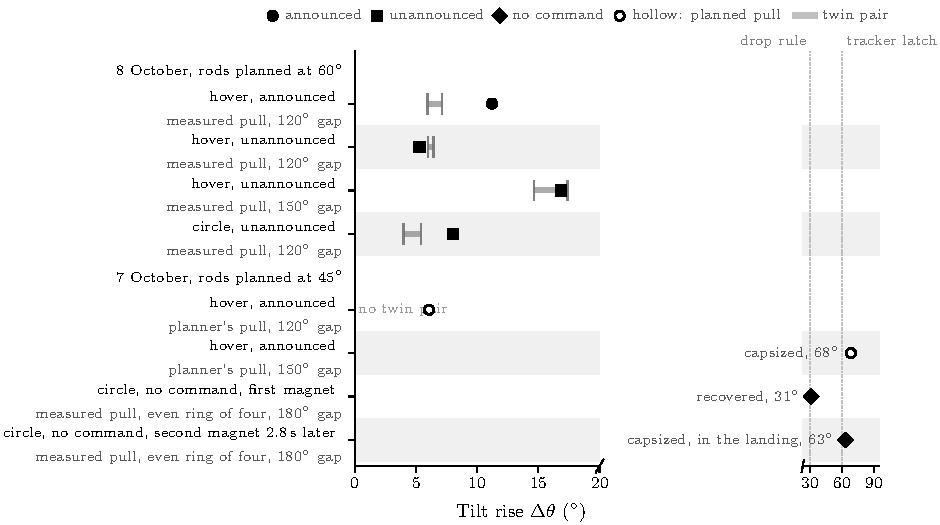
\includegraphics[width=\textwidth]{Images/releases.pdf}
\caption[Every release on the rig]{Every release on the rig to 8 October, one row per event, grouped by the day and
the rod plan: the ring's tilt rise $\Delta\theta$ (the departure of its tilt vector from its mean over the 5\,s
before the event, over the event to LAND or to the fleet's latch) as a marker, filled for the measured rod pull and
hollow for the planner's pull, shaped by how the release came (announced, unannounced, or a magnet letting go with no
command); the grey bar with end ticks is the range of the twin pair flown on the same configuration, cut at the rig
flight's hold, and rows without one say so. The two capsizes and the one recovery sit on the broken axis against the
30$^\circ$ drop rule, which these flights predate, and the trackers' 60$^\circ$ latch. The 7 October circle flew the
even ring of four, whose three survivors leave a 180$^\circ$ gap; it lost two magnets 2.8\,s apart, recovered from the
first, and capsized on the second during the landing, so that row's pre-window holds the first recovery.}
\label{fig:F10}
\end{figure}

\begin{figure}[htbp]
\centering
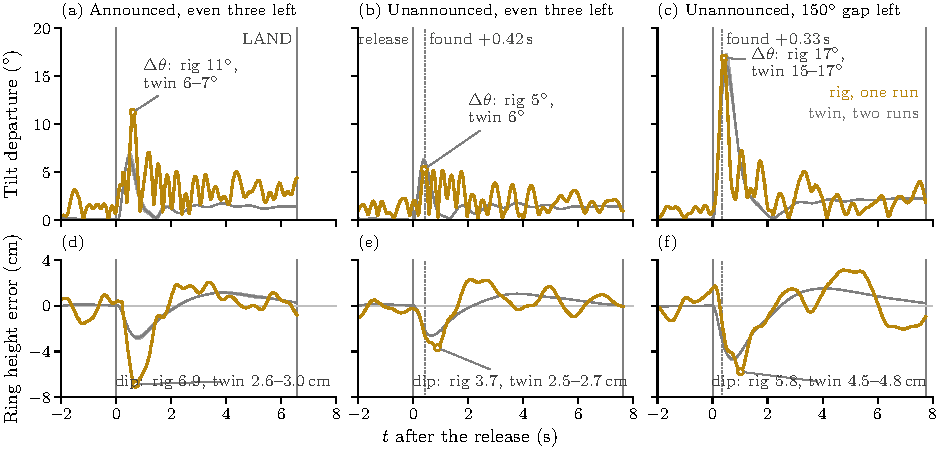
\includegraphics[width=\textwidth]{Images/rig_detach.pdf}
\caption[Releases on the rig against the twin]{Releasing one UAV of four on the rig, 8 October (gold, one run each)
against the rig twin (grey band and line: two runs, nearly identical), aligned on the release (dotted). Announced: the
planner releases the magnet and drops the UAV from its optimisation at once. Unannounced: the magnet is switched off
without telling the planner, which finds the release from the stretched rod (second dotted line, 0.33--0.42\,s after
the release on the rig). (a--c) The ring's tilt departure: the length of its tilt vector's difference from that
vector's mean over the 5\,s before the release, so that the rig ring's own rocking in hover (1--1.4$^\circ$ about its
mean) is measured about the mean rather than added to the rise; the marker and label give the tilt rise
$\Delta\theta$, the departure's peak from the release to LAND, with the twin cut at the rig flight's hold. (d--f) Ring
height error, measured minus planned (negative: below). Announced: the rig rose 11$^\circ$ against the
twin's 6--7$^\circ$, and its lowest height error was 6.9\,cm against 2.6--3.0\,cm. Unannounced: the rig rose
5$^\circ$ against 6$^\circ$ and 17$^\circ$ against 15--17$^\circ$, and its lowest height error was about 1\,cm
lower than the twin's (3.7 against 2.5--2.7\,cm; 5.8 against 4.5--4.8\,cm). (Table~\ref{tab:T8b} measures the dip
against the pre-event mean instead.) Rig traces end at the fleet's LAND.}
\label{fig:rig_detach}
\end{figure}

\begin{figure}[htbp]
\centering
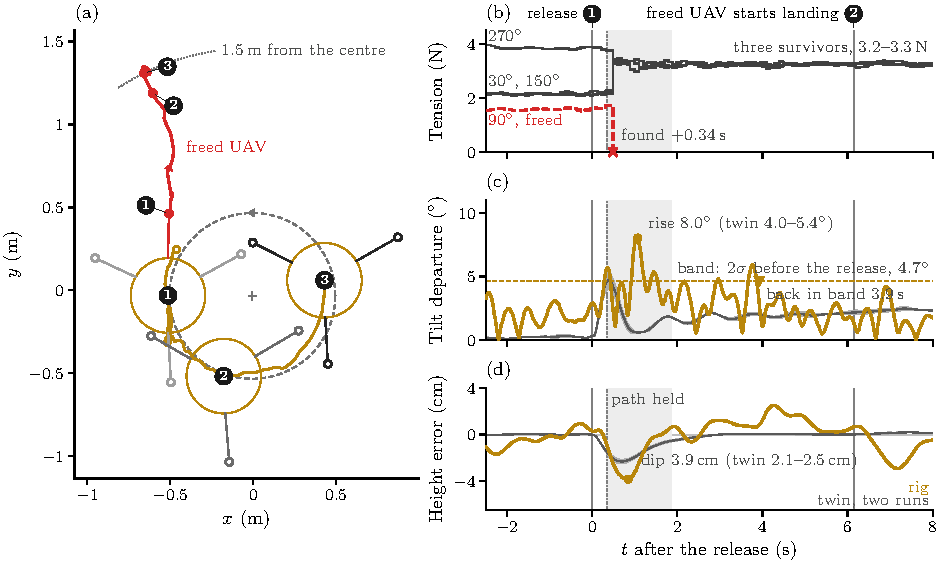
\includegraphics[width=\textwidth]{Images/rig_circle_detach.pdf}
\caption[Unannounced release during the circle on the rig]{An unannounced release during the circle on the rig, 8
October: four UAVs carry the 0.86\,kg ring at 1.0\,m round a circle of radius 0.5\,m at 0.125\,m/s, on plates 3, 7, 9
and 11, and the magnet of the UAV on plate 9 is switched off without telling the planner. (The panels print each
plate's counter-clockwise azimuth: 30$^\circ$ is plate 11, 90$^\circ$ plate 9, 150$^\circ$ plate 7, 270$^\circ$ plate
3.) (a) Plan view: the circle (dashed; +, its centre; arrow, the direction of travel), the ring's centre from 2.5\,s
before the release (open circle) to LAND (gold), and the fleet at three instants, each numbered at the ring's centre
and at the freed UAV: the ring (thin gold circle), the carriers with their rods to their plates (grey, darker for
later instants) and the freed UAV (red, with its path to LAND). 1: the release; 2: the freed UAV starts its own
landing, 6.1\,s later; 3: the fleet's LAND, 14.0\,s after the release, with the freed UAV 1.5\,m from the circle's
centre (dotted arc). (b)--(d) The 2.5\,s before the release to 8\,s after it. (b) The planner's tension per UAV: the
freed UAV's (dashed) stays in the plan until the planner finds the release from its stretched rod 0.34\,s after the
release (dotted line) and drops it at its next logged tick (cross); the three survivors then share the ring at
3.2--3.3\,N each, from 2.1--3.9\,N before. Grey band: the path held for 1.5\,s from the detection. (c) The ring's tilt
departure and (d) ring height error (measured minus planned): the rig (gold, one run) against the twin flying the
same configuration (grey band and line: two runs, nearly identical). The twin's departure peaks once, at
4.0--5.4$^\circ$ 0.4\,s after the release (cut at the rig's hold); the rig's spikes to 5.7$^\circ$ at the same time
and peaks at 8.0$^\circ$, its tilt rise $\Delta\theta$, 1.1\,s after it. Dashed: the band of the rig's own rocking
before the release, twice its standard deviation (4.7$^\circ$); the triangle marks where the rig's departure is back
inside it for a second, 3.9\,s after the release. Its lowest height error is 3.9\,cm against the twin's 2.1--2.5\,cm.}
\label{fig:rig_circle_detach}
\end{figure}

\paragraph{Against the rig's no-event floor.} With nothing happening, the same statistic over a 7\,s hover window
reads 4.8$^\circ$ on average across 23 such windows (95th percentile 6.0$^\circ$) and 6.3$^\circ$ over a 15\,s path
window (43 windows, 8.3$^\circ$), because it takes the largest excursion of a two-dimensional vector over the window.
L4 and L6 lie above every no-event window. On raw $\Delta\theta$, L5 lies inside the hover null and L7 inside the
path null. Scaled by each window's own pre-event rocking, L1 and L7 do not separate from it, L5 does
(4.5\,$\sigma_\mathrm{pre}$ against a null median of 3.3). [The hover null rests on two 7 October carry flights; the
path null mixes the planned and the measured pull.] L1's absolute peak came 0.1\,s before LAND; its first second
peaked at 4.6$^\circ$, and its $\Delta\theta$ exceeds its peak because the tilt swung to the far side of a
1.5$^\circ$ pre-event lean.

\paragraph{How the ring was lost.} Every ring lost on the rig began with a magnet letting go with no command
(Figure~\ref{fig:F11}). In L2 the planner raised the largest survivor's tension, within the first second after the
resize, by up to 2.75\,N (+1.8\,N at its first solve), against the 1.61\,N the static redistribution of that layout
asks for, and a survivor's magnet let go 0.17\,s after the release at 2.6$^\circ$ of tilt: the first solve's +1.8\,N against the 1.61\,N of statics came before the release, where on 8 October, on
the measured pull, the same layout's step was 1.74\,N and the ring recovered from 17.8$^\circ$. In L3 a magnet let go
in a steady circle at 0.9$^\circ$ of tilt with every rod at 3.0\,N. Two more let go after the rods were planned at
60$^\circ$, both in the attach flights with three carriers. On 14 October (L10) the three-carrier lift ran with the
carriers' commands at 42--44\,Hz instead of 50 under the combined attach stack, the ring bobbed at about 1\,Hz with a
growing amplitude, every pose and command stream froze for 0.25\,s, and half a second later one carrier's magnet let
go (whether the slowed loops or the freeze caused it is open); with two carriers left and the drop rule then
off in that mode, the ring capsized and the fleet was disarmed about 1\,m up. The drop rule has been on in every mode
since. On 15 October (L11) a carrier let go of plate 7 in a steady hover with nothing touching it and its pack at
21.9\,V; the ring tilted to 36.8$^\circ$, the drop rule switched every magnet off, and every carrier landed and was
disarmed alone. The magnets stay on from each launch, and nothing records their current or temperature, so whether
heat or a low pack weakened that hold is open.

\begin{figure}[htbp]
\centering
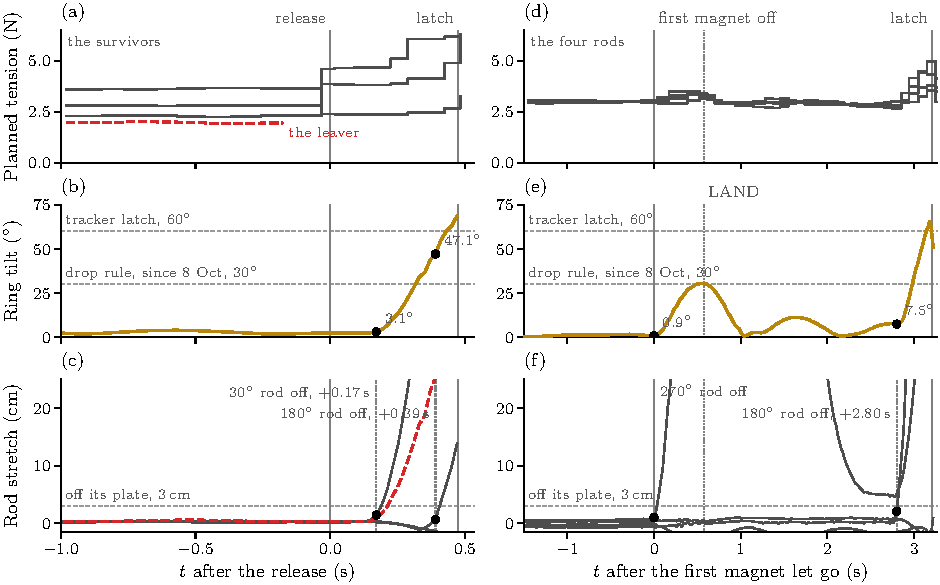
\includegraphics[width=\textwidth]{Images/magnet_anatomy.pdf}
\caption[How the ring was lost]{How the ring was lost on the rig on 7 October, twice, both with the rods planned at
45$^\circ$. (The panels print each rod's counter-clockwise azimuth: 30$^\circ$ is plate 11, 90$^\circ$ plate 9,
180$^\circ$ plate 6, 270$^\circ$ plate 3.) Left, an announced release from plate 9 of a hover on plates 3, 6, 9 and 11
(a 150$^\circ$ gap left), on the planner's pull: (a) the planned tension per rod, the leaver's dashed, with the
survivors' step at the resize (2.8 to 4.6\,N and 2.3 to 3.8\,N on the two rods beside the gap); (b) the ring's tilt;
(c) each rod's measured length over its own, so that a rod leaving its plate shows as a rise: 0.17\,s after the
release the rod on plate 11 let go with no command, at 2.6$^\circ$ of tilt, and the rod on plate 6 followed at
0.39\,s; the trackers latched the fleet at 60$^\circ$ of tilt 0.47\,s after the release. Right, the circle at
0.125\,m/s on the measured pull with four rods on the even ring: (d) the planned tensions, 3.0\,N each; (e) the tilt;
(f) the rod on plate 3 let go with no command at 0.9$^\circ$ of tilt and the ring recovered from 31$^\circ$; the
operator's LAND came 0.6\,s after it, and during the descent the rod on plate 6 let go, at 7.7$^\circ$, and the ring
capsized. Dotted: the 30$^\circ$ drop rule and the trackers' 60$^\circ$ latch; the freed rods leave the panel.}
\label{fig:F11}
\end{figure}

\paragraph{A constant offset.} All four releases of 8 October held the ring 5.3--6.8\,cm from its reference before
the release, against 2.1\,cm in the measured-pull hover of the day before, because they ran the reference-shift
height integral (the model integral was not yet allowed on a fleet that changes size) where the carry flights ran
the model integral (Section~\ref{sec:res_rig_integral}). The model integral is now kept through a resize; L8 and L9
fly it.

\subsubsection{One release in the twin}
\label{sec:res_twin_release}

Figure~\ref{fig:detach} shows one unannounced hover release in the twin on the freeze code tree, the cell the rig's
next hover release flies: four UAVs on plates 3, 7, 9 and 11, the magnet on plate 9 switched off without telling the
planner, the measured pull and the model integral. The planner finds the loss from the stretched rod and, re-solved
for the three survivors on their actual plates, hands the released UAV's share to them in one tick: the three end
equal, as the statics of the even triangle say (Section~\ref{sec:reconfig}). Over the three runs of this arm (the
release moved by 0.5\,s between them, so only the first is exactly the rig cell's configuration) the tilt rise was
5.5--7.7$^\circ$, the ring dipped 2.7--3.8\,cm, it was back in its band (Section~\ref{sec:metrics}) 3.9--4.2\,s after
the release, and every run landed with the freed UAV disarmed alone.

\begin{figure}[htbp]
\centering
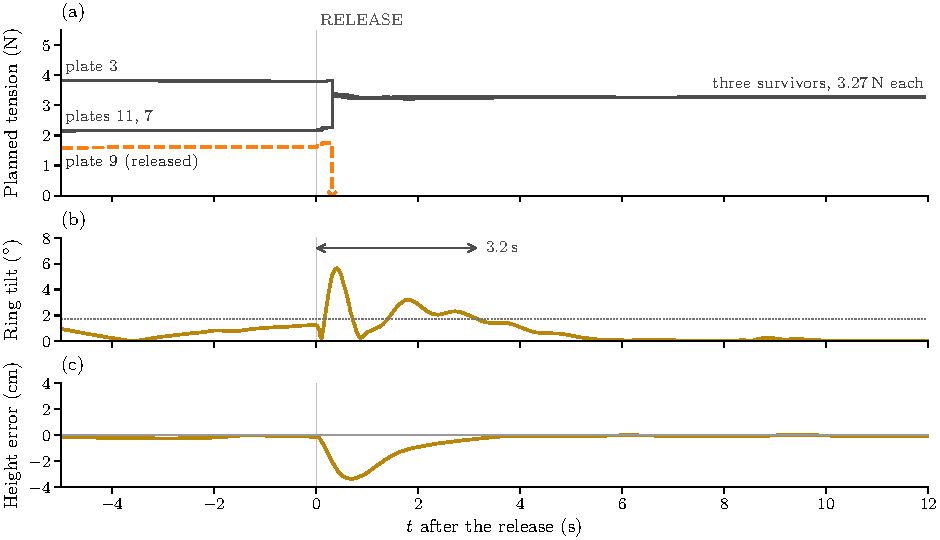
\includegraphics[width=\textwidth]{Images/detach.pdf}
\caption[One release in the twin]{An unannounced release of one UAV of four in the rig twin, hover at 1.0\,m, UAVs on
plates 3, 7, 9 and 11 (Figure~\ref{fig:geometry}), the measured rod pull and the model integral; one run. (a) The
rod tension planned for each UAV; the UAV on plate 9 (dashed) is released at RELEASE and dropped from the plan when the
planner finds the loss, and the three survivors, now an even triangle, share the load equally. (b) Ring tilt; dotted:
the hover's own maximum plus 0.5$^\circ$; arrow: the time until the tilt stays below it. (c) Ring height error
against the 1.0\,m target. The tensions are planned, since the twin does not measure them.}
\label{fig:detach}
\end{figure}

\subsubsection{The levers in the twin}
\label{sec:res_levers}

\paragraph{The pull source on an unannounced release.} The frozen one-degree-of-freedom model (Section~\ref{sec:discussion})
predicts that on an unannounced release the measured pull, which follows the rod from its first samples, beats the
planner's pull, which flies the four-UAV shares until the resized plan arrives (a new prediction). In the twin cell
the prediction names (Figure~\ref{fig:F10b}), the measured rod pull kept the tilt rise to 5.5--7.7$^\circ$ where the
planner's pull let it reach 16.6--17.1$^\circ$; the means differ by 10.4$^\circ$ against the 4.4$^\circ$ the rule
requires, so the prediction is confirmed for this cell. The pair settles the sign, not the mechanism: the two arms do
not start from the same state, since on the planner's pull the ring hung 2.0$^\circ$ tilted at a steeper rod
elevation before the release. The announced half of the crossover, where the planned pull is predicted to win, has
not been flown.

\begin{figure}[htbp]
\centering
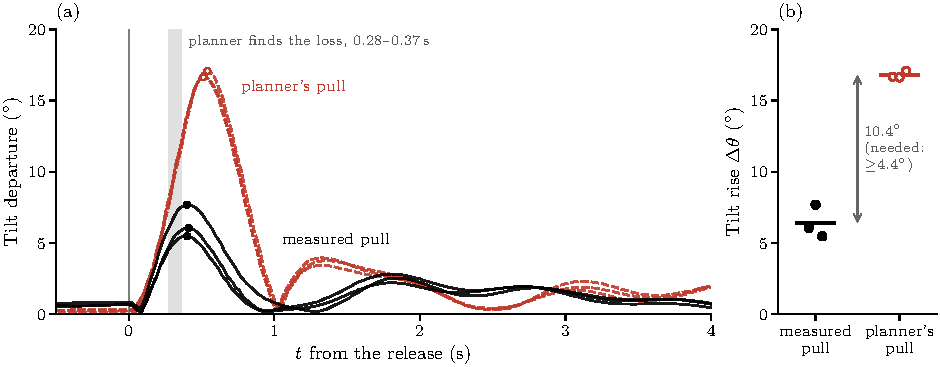
\includegraphics[width=\textwidth]{Images/crossover.pdf}
\caption[The pull source on an unannounced release]{An unannounced release in the twin, one cell: four UAVs
hover the 0.86\,kg ring at 1.0\,m from plates 3, 7, 9 and 11, and the magnet on plate 9, the smallest share, opens
without telling the planner, leaving a 120$^\circ$ gap; the model integral; every link rigid; three runs per pull
source, the release instant moved by 0.5\,s between runs. (a) The ring's tilt departure (its tilt vector's distance
from its mean over the 5\,s before the release) against time, black with the survivors flying the measured rod pull,
red with them flying the planner's pull; marker: each run's tilt rise $\Delta\theta$, the largest departure up to 15\,s
after the release; grey: the planner finding the loss and resizing to three UAVs, 0.28--0.37\,s after the release over
the six runs. (b) $\Delta\theta$ per run (filled: measured pull; hollow: the planner's pull) and the arm means:
5.5--7.7$^\circ$ against 16.6--17.1$^\circ$. The means differ by 10.4$^\circ$ against the 4.4$^\circ$ the resolution
rule frozen before the runs requires, so the pair resolves with the predicted sign. The two arms do not start from the
same state: on the planner's pull the ring hung 2.0$^\circ$ tilted before the release and again after it, on the
measured pull 0.4--0.8$^\circ$ before and level after.}
\label{fig:F10b}
\end{figure}

\paragraph{The support margin.} The statics of Section~\ref{sec:reconfig} predict a larger transient for a smaller
margin, and the twin confirms it on the measured pull (Figure~\ref{fig:F12}b): moving the third survivor so that the
largest gap grows from 120 to 165$^\circ$ took the tilt rise from 5.5--7.7$^\circ$ at a 112\,mm margin to 7.8--9.1,
16.7--17.0 and 27.9--28.1$^\circ$ at 86, 58 and 29\,mm. Both pairs on rig plates resolve with the predicted sign (the second also differs in
the drop rule, off at 180$^\circ$), and no neighbouring pair resolves the other way; the step from 112 to 86\,mm is in the predicted direction but unresolved
at two runs. At a 29\,mm margin the ring came within 1.9--2.2$^\circ$ of the drop rule. With no margin (a 180$^\circ$
gap) three UAVs cannot hold the ring: with the drop rule off, the trackers' 60$^\circ$ latch disarmed the fleet in the
air 0.6\,s after the release, and on the default rules the planner's gap rule dropped the ring when it found the loss. At a 150$^\circ$ gap the planner's pull reached the drop rule in both runs and the ring was
dropped, which also confirms the pull-source prediction at that margin; with the measured pull every peak at gaps up
to 150$^\circ$ stayed under 30$^\circ$ (largest 16.9$^\circ$). The bar frozen as ``no run at gaps up to 150$^\circ$
reaches the drop line'' is therefore falsified as written, by the planner's pull. The twin has no magnet holding limit:
the curve speaks for the planner and the statics, not for a margin of safety on the rig.

\paragraph{What detecting the release buys.} On the planner's pull, detection decides the outcome: with detection off
the planner never resizes, and the tilt rise reached 28.2$^\circ$ in all three runs against 16.6--17.1$^\circ$ with it,
the tilt creeping to within 1.5--2.4$^\circ$ of the drop rule (confirmed, a new prediction). On the measured pull,
detection made no difference the rule could resolve at three runs (means 5.6 and 6.4$^\circ$, with the detection-on
arm's own range 2.2$^\circ$), as the pure model predicts. What detection does buy at landing in this cell is the freed
UAV's own landing: with detection off it never learns that it left and lands with the ring; on the three UAVs still on
the ring the landing lean is unresolved on either pull source. With detection off on the planner's pull, the freed UAV,
still flying its share of a load it no longer carried, came down sideways and tipped on the twin's floor, and its
envelope disarmed the fleet at landing in all three runs, a twin result not shown for the rig.

\paragraph{Carrying a circle with no event.} On the 60$^\circ$ circle with no release, the planner's pull tracked
better in the twin than the measured pull, 0.49--0.58 against 0.87--0.98\,cm mean path error (the even ring, two runs
each, 0.09\,cm over the frozen floor), but held height and tilt less evenly (height standard deviation 0.41--0.42
against 0.10\,cm). This is a replication of the earlier stack's order and not the rig's falsifier, which needs the
planned-pull 60$^\circ$ circle on the rig (K4).

\begin{figure}[htbp]
\centering
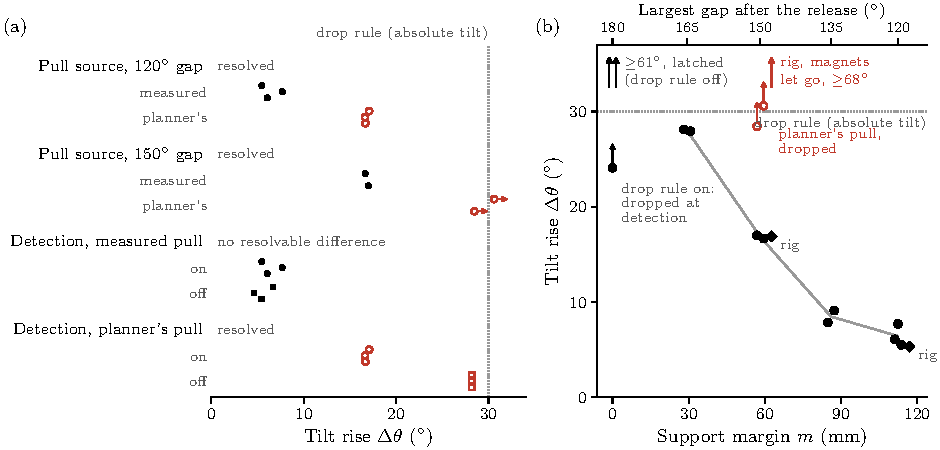
\includegraphics[width=\textwidth]{Images/levers.pdf}
\caption[The other levers]{The other levers in the twin: unannounced hover releases, the model integral, every link
rigid; one marker per run; arrow or triangle: a lower bound, the run cut where the ring was dropped or the fleet
latched. (a) One-variable pairs, each headed by its variable: the pull source with a 120$^\circ$ and a 150$^\circ$ gap
left, and detecting the release on and off (off: the planner never resizes) on each pull source; filled: the measured
rod pull; hollow: the planner's pull; right: the pair under the resolution rule frozen before the runs. With detection
off on the planner's pull the largest departure came 9.5--10.7\,s after the release, the tilt creeping to within
1.5$^\circ$ of the drop rule. (b) $\Delta\theta$ against the support margin $m = r\cos(g/2)$, $r = 0.225$\,m, that the
largest gap $g$ left between the three remaining UAVs gives (top axis), on the measured pull, the line through the
means: 5.5--7.7$^\circ$ at 112\,mm, 7.8--9.1$^\circ$ at 86\,mm, 16.7--17.0$^\circ$ at 58\,mm and 27.9--28.1$^\circ$ at
29\,mm. At zero margin, with the drop rule off, the trackers' 60$^\circ$ latch disarmed the fleet in the air 0.6\,s
after the release (arrows); on the default rules the planner's gap rule dropped the ring when it found the loss (filled
triangle). Hollow triangles: the planner's pull at 58\,mm, cut by the trackers' 30$^\circ$ drop rule in both runs.
Diamonds: the rig's two unannounced hover releases of 8 October (the reference integral, the freed UAV landing with the
fleet, $\Delta\theta$ up to their LAND 7.6--7.7\,s after the release); red arrow: the rig's announced release on the
planner's pull with the rods planned at 45$^\circ$, in which two magnets let go (Figure~\ref{fig:F11}). The twin has no
magnet holding limit: the curve speaks for the planner and the statics, not for a margin of safety on the rig.}
\label{fig:F12}
\end{figure}

Appendix~\ref{sec:app_levers} gives every pair in one table with its frozen sign, its label and its verdict.

\subsubsection{The switch itself}
\label{sec:res_switch}

The resize is a switch between two optimal control problems of different size, and Table~\ref{tab:T10} measures it at
the first live solve of the smaller problem. No solve failed at any of 26 switches, 20 in the twin and 6 on the rig:
every first solve returned status 0 from the warm path, with residuals in the range of the last solve of the larger
problem one tick before. On the rig the first three-UAV solve took 24--28\,ms, and in the second after it 2 of 66
solves passed the 60\,ms budget, none of them cut short. On the measured pull the survivors' throttle step at the
switch is the release's and not the switch's: the twin's detection-off runs, which never switch, read the same in the
same window. On the planner's pull the step is the planned share arriving, 11.4--11.9\,\% of hover throttle in the
120$^\circ$ cell against 2.3--3.3\,\% without a switch. The gap to an offline solve run to convergence is not computed, since the planner keeps a
problem only when its solve fails.

% generated by tools/thesis_freeze_tables.py; run ids in docs/figures/PROVENANCE.md
\begin{table}[htbp]
  \centering
  \footnotesize
  \setlength{\tabcolsep}{3pt}
  \caption[The switch itself]{The switch itself (T10): the planner's first solve of the smaller problem when a UAV
  leaves, and the second after it; $n$ switches. Status: the solver's status at the first solve, then the failed solves
  in the second after it. KKT residual: stationarity and dynamics at the first solve, the largest in the row. Solve time, rig only: the first solve and
  the longest in the second after it (60\,ms budget). Throttle step: the survivors' largest throttle
  departure in the 0.3\,s after the switch, over their hover throttle; in brackets, the same statistic at the planner
  ticks of the steady hover before.}
  \label{tab:T10}
  \begin{tabularx}{\textwidth}{>{\raggedright\arraybackslash}p{1.6cm}>{\raggedright\arraybackslash}Xcccc}
    \toprule
    Switch & Data ($n$) & Status; failed & KKT residual (stat / eq) & Solve time (ms) & Throttle step (\%) \\
    \midrule
    Leave, announced & Rig, planner's pull$^a$ (2) & 0; 0 of 22 & $1.1\times10^{-3}$ / $1.1\times10^{-7}$ & 24--28; 58--60 & 12.6--15.8 (1.2--3.9) \\
     & Rig, measured pull (1) & 0; 0 of 11 & $6.5\times10^{-5}$ / $2.4\times10^{-8}$ & 26; 35 & 15.9 (7.3) \\
    Leave, unannounced & Twin, measured pull, gap 120--165$^\circ$ (13) & 0; 0 of 130 & $3.8\times10^{-4}$ / $2.3\times10^{-7}$ & -- & 1.9--5.7 (0.4--0.9) \\
     & Twin, measured pull, gap 180$^\circ$$^b$ (2) & 0; 0 of 21 & $3.9\times10^{-4}$ / $1.7\times10^{-8}$ & -- & 11.5--12.1 (0.4--0.5) \\
     & Twin, planner's pull, gap 120--150$^\circ$$^c$ (5) & 0; 0 of 34 & $9.9\times10^{-5}$ / $2.4\times10^{-8}$ & -- & 11.4--16.8 (0.4--0.5) \\
     & Rig, measured pull (3) & 0; 0 of 33 & $3.3\times10^{-4}$ / $2.9\times10^{-7}$ & 25--26; 32--62 & 9.2--13.3 (6.8--9.4) \\
    Join (hand-over) & [the join code tree] & [\dots] & [\dots] & [\dots] & [\dots] \\
    \bottomrule
    \multicolumn{6}{>{\raggedright\arraybackslash}p{\dimexpr\textwidth-2\tabcolsep}}{\footnotesize $^a$\,Rods planned at
    45$^\circ$; in one of the two flights two magnets then let go and the ring capsized (Figure~\ref{fig:F11}).
    $^b$\,No margin, the drop rule off: the fleet latched 0.4\,s after the switch. $^c$\,In 2 of 5 runs the trackers'
    30$^\circ$ rule dropped the ring 0.2\,s after the switch; the window ends there.} \\
  \end{tabularx}
\end{table}


\subsubsection{The freed UAV}
\label{sec:res_freed}

On the rig on 8 October the freed UAV's own landing did not finish: in all four releases it floated above its resting
height until the fleet's disarm at the end of the landing dropped it about 0.3\,m (Figure~\ref{fig:departed_landing}a),
and the twin shows the same stall (Figure~\ref{fig:departed_landing}b). Its height reference is now pressed down to its
own resting height, and once there it is disarmed alone, without waiting for the fleet
(Figure~\ref{fig:departed_landing}c). On the freeze code tree the freed UAV was disarmed alone 0.27--0.43\,s after it
first reached its rest, within 2\,mm of it and before the fleet landed, in every hover and circle release (five runs);
no carrier was disarmed before the fleet landed. On the rig the rule has so far acted only in the drop of 15 October
(L11), where every carrier landed by itself and was disarmed alone.

\begin{figure}[htbp]
\centering
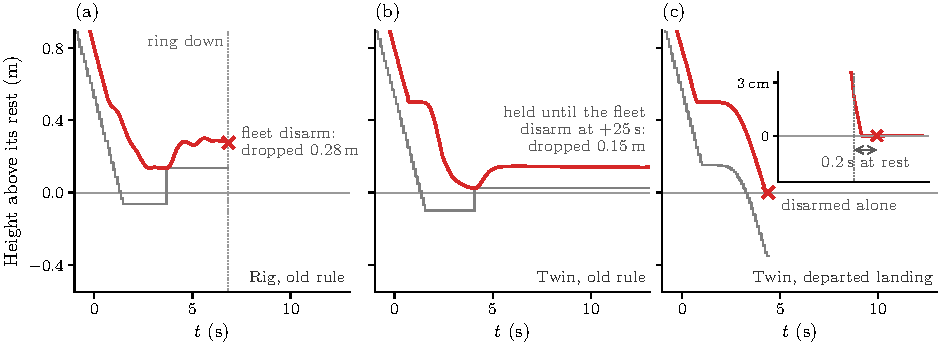
\includegraphics[width=\textwidth]{Images/departed_landing.pdf}
\caption[A freed UAV's own landing, old rule and departed landing]{A UAV landing by itself off the ring, the same UAV
(the fourth) in three cases, aligned where it passes 0.8\,m on the way down; solid: its height above its own resting
height, grey: its height reference until it is disarmed, cross: its disarm, dotted: the ring reaching the floor. (a)
Rig, old rule: its touchdown test fired 0.14\,m above its rest, the reference froze there, the UAV rose to 0.28\,m and
hovered until the fleet's disarm at the end of the landing dropped it 0.28\,m. (b) Twin, old rule: the same stall, held
0.15\,m up for 25\,s until the fleet's disarm dropped it. (c) Twin, departed landing: the reference is pressed below the
resting height until the UAV is there, and it is disarmed alone 0.2\,s after reaching it (inset). The plateau at 0.5\,m
in (b) and (c) is the UAV standing on the tip of its rod before the rod tips over.}
\label{fig:departed_landing}
\end{figure}

\pendingfig{fig:rig_departed}{The freed UAV's own landing on the rig with the departed landing: pushed to its resting
height and disarmed alone.}{the rig's hover and circle releases (L8, L9), the next rig day}

\subsubsection{Losing a second carrier: the drop}
\label{sec:res_drop}

A loss that leaves fewer than three carriers, or a ring tilted past 30$^\circ$, drops the ring
(Section~\ref{sec:safety}). On the freeze code tree in the twin, a second loss after a first, and a first release that
leaves a 240$^\circ$ gap, were each flown twice: the ring was dropped 0.22--0.23\,s after the loss, no UAV tilted past
13.6$^\circ$ or climbed more than 0.18\,m, and every UAV was down (below 0.15\,m) within 8.5--8.9\,s and disarmed
0.10--0.11\,m above the floor, with no fault. Which rule fires first is a race: in one of the 240$^\circ$ runs the
planner's gap rule fired at the detection, 2\,ms ahead of the trackers' tilt request, with the ring already at
33.7$^\circ$; in the others the trackers' request came first. The margin to the trackers' 60$^\circ$ latch is thin,
0.06--0.12\,s in the twin. On the rig the rule fired once, on 15 October (L11, above), and landed every carrier.

\paragraph{Answer to RQ2.} What sets the ring's transient when a carrier leaves is, first, geometry: in the twin the tilt
rise grew as the support margin the leaver leaves behind shrank, from 5.5--7.7$^\circ$ at 112\,mm to
27.9--28.1$^\circ$ at 29\,mm, and with no margin three UAVs cannot hold the ring. Second, the pull source the survivors
fly on: in the two twin hover cells flown (120 and 150$^\circ$ gaps) the tilt rise was smaller on the measured pull than
on the planner's pull, a sign and not yet a mechanism, and on the planner's pull detecting the release held the rise at
17$^\circ$ where without it the tilt crept to within 1.5--2.4$^\circ$ of the drop rule.
The resize itself is a clean switch: no solve failed at 26 switches. On the rig three UAVs carried the ring on through
five of six commanded releases with tilt rises of 5.3--16.9$^\circ$. What loses a ring is a magnet letting go: all four
rings lost on the rig began that way, twice after the rods were planned at 60$^\circ$, and the drop rule, on in every
mode since 14 October, landed the fleet when it happened again on 15 October.


% res_join.tex -- Results 4.3: joining the team (RQ3). 17 Oct (v3_full): sim_attach.tex and skel_join.tex merged.
% The join tables fly on a second code tree after the 21-22 Oct rig day (Wesley 16 Oct, inventory decisions (1), (2),
% (9), (11)): T11 and F14 re-flown on the co-motion confirmation; T12 two hover runs under a card, the circle
% exploratory; the push-abort clearance bar is the newcomer's own clearance. The 12 Oct contact-and-lift T11 and F14 are
% STALE-MECH (one line of history in App D). Tonight's exploratory join re-fly (17-18 Oct) is not thesis evidence.
% Rig record: docs/reports/supervisor_brief_2026-10-16.md and morning_report_2026-10-16.md (rig bags re-read), registry
% RIG-1014-t6h_4, RIG-1015-a1, a2_2, a3_2; the offline replay: card docs/experiments/2026-10-15_attach_comotion_rig.md
% (baseline; tools/proof_replay.py). Fault coverage: drop_takes_back card (16 Oct, twin, SUPPORTED WITH CORRECTIONS),
% quad4_tilt_cut rev 4 (week5 R1702-R1705, 4 of 4, exploratory), land_every_phase (9 Oct), newcomer_land_abort.

\subsection{Joining the team}
\label{sec:res_join}

This section answers RQ3: what must be observed before a UAV flown by another controller is admitted to a carried
ring, and what does admission cost the ring? It is the least complete of the three. The confirmation was rewritten on
14 October, after the rig's first catch was rejected by the proof of the day, and the twin claim for the new
confirmation flies on the join code tree after the rig day of 21--22 October; its tables and figures below are
placeholders sized for that batch. What is in hand is the contract itself (Section~\ref{sec:admission}), an offline
replay of the new confirmation on the rig's one catch, the rig's attach record so far, and the fall-backs.

\subsubsection{The admission contract in the twin}
\label{sec:res_contract}

Figure~\ref{fig:F14} and Table~\ref{tab:T11} will give the contract on the join code tree: the collaborator's
controller flies the newcomer down onto plate 9 of a carried ring, and this work confirms the catch from motion
capture, switches the radio and folds the newcomer in, or takes it back. Smoke runs of the co-motion confirmation in
the twin admitted the newcomer, folded it in and landed (exploratory, one run per code tree); the twin's rigid tether
cannot go slack, so the rig's thresholds stay on the rig side.

\pendingfig{fig:F14}{The co-motion confirmation in the twin: a newcomer flown by the collaborator's controller comes
down onto plate 9 of a hovering ring and the catch is confirmed from motion capture alone. (a) Heights of the
newcomer's body, its magnet tip and the plate point; (b) the tip's drift from its contact point in the plate frame,
against the 6\,mm confirmation and the 45\,mm loss; (c) the newcomer's throttle across the switch of its radio; (d) the
ring's tilt departure against the 5$^\circ$ bar.}{the hover attach runs of the join claim, on the join code tree}

\begin{table}[htbp]
  \centering
  \footnotesize
  \caption[The twin claim for the join]{The twin claim for the join (T11): the collaborator's controller flies the
  newcomer to contact and this work's co-motion confirmation admits it. Ranges over $n$ runs on one code tree; the
  ring's tilt rise on the release metric with the contact as the event; clearance: the newcomer's body and rod to every
  carrier, and in the push abort the newcomer's own. [Every cell: the join claim on the join code tree, after the
  21--22 October rig day, then the reviewer.]}
  \label{tab:T11}
  \begin{tabularx}{\textwidth}{XcYYYYl}
    \toprule
    Claim line & $n$ & Contact to confirmation (s) & Throttle step (\%) & Ring tilt rise ($^\circ$) & Clearance (m)
      & Reviewer \\
    \midrule
    Attach, hover & [\dots] & [\dots] & [\dots] & [\dots] & [\dots] & [\dots] \\
    Take-back, hover & [\dots] & -- & -- & [\dots] & [\dots] & [\dots] \\
    No catch, hover & [\dots] & -- & -- & [\dots] & [\dots] & [\dots] \\
    LAND during the confirmation & [\dots] & -- & -- & [\dots] & [\dots] & [\dots] \\
    No catch, circle & [\dots] & -- & -- & [\dots] & [\dots] & [\dots] \\
    LAND take-back, circle & [\dots] & -- & -- & [\dots] & [\dots] & [\dots] \\
    Push abort & [\dots] & -- & -- & [\dots] & [\dots] & [\dots] \\
    Re-attach & [\dots] & [\dots] & [\dots] & [\dots] & [\dots] & [\dots] \\
    \bottomrule
  \end{tabularx}
\end{table}

\paragraph{Counterfactuals.} [On the join code tree: the newcomer seeded at its full share against 0.1\,N; the
confirmation without its plate-motion condition; the hand-over step against a thrust blend of the kind TRADY uses
\cite{sugihara2023trady}.]

\subsubsection{The confirmation on rig noise}

The twin's magnet catches at the instant of contact and its ring hardly moves, so the confirmation's plate-motion and
taut-tether conditions can only be judged on rig data. Replayed offline over the flights of 14 October with the rig's
thresholds (a 24\,mm catch radius and each flight's own free hang), the co-motion rules confirm the one catch of that
day 2.81\,s after its contact, the tip drifting 1.1\,mm in the plate frame while the plate moved 16\,mm, and find no
contact and no false confirmation in the other descents. [False accepts and rejects over every rig recording with a
descent, and the rig thresholds set from them.]

\subsubsection{On the rig}
\label{sec:res_join_rig}

Eight attach flights on 14 and 15 October, the collaborator's controller flying the newcomer from its mat to plate 9
of a ring held at 1.0\,m by three carriers, gave one contact and no fold-in (exploratory). In that contact the magnet
held plate 9 through three lifts, and the proof of the day rejected it on its taut check; the co-motion confirmation
that replaced it confirms it offline (above). In the other descents the magnet was inside the catch radius at the
bottom only 22\,\% of the time; three bottom holds ended with the tip at plate height 3.3--4.3\,cm along the ring from
the plate point, past the edge of the 60\,mm plate; and the ring bounced about 0.8\,cm at 1.8\,Hz under the newcomer,
which followed the bounce 0.25\,s late. In one flight the collaborator's match check never held long enough for a
descent (42\,s), and in another the newcomer's tether passed 0.10\,m from a carrier on the way in. One of these flights
also lost the ring when a carrier's magnet let go (L11, Section~\ref{sec:res_leave}). The attach on the rig is
therefore limited by getting the magnet onto the plate, which is the collaborator's controller's task and the plate's
size, before any admission is tested. The response is hardware first: 90\,mm plates, inside whose catch radius the
magnet would have been 49\,\% of the time at the bottom on these flights instead of 22\,\%, and 1\,m tethers, which give
the newcomer 0.70\,m of room from the nearest carrier instead of 0.45\,m; both are planned for the next rig day.

\pendingfig{fig:F15}{The first attaches on the rig: the newcomer's descent onto plate 9, the contact, the
confirmation, the switch of its radio and the fold-in, with the ring's tilt against the 5$^\circ$ bar for the thesis
and the 10$^\circ$ safety limit.}{the attach flights of the 21--22 October rig day}

\subsubsection{Fault coverage and authority}
\label{sec:res_join_faults}

Every fall-back of Section~\ref{sec:safety} has been flown in the twin from the phase it guards, the attach
phases on the earlier attach sequence (Appendix~\ref{sec:app_faults}). LAND from every phase of an attach landed and
disarmed every UAV except in one run, LAND 0.5\,s after a weld, where the twin's rigid rod tipped the newcomer (on the code tree of 9 October, before the
collaborator's controller flew the attach). A fault on a newcomer in transit disarms it alone and lands the carriers.
When the ring is dropped while the collaborator's controller flies the newcomer, the newcomer is taken back on the
drop tick, kept at least 0.5\,m from every carrier and set down at its rest 14--17\,s later (twin only); without that
switch the twin reproduced the rig's problem, its newcomer flying on towards the fallen ring. The tilt cut caught an
injected upset on a newcomer under the collaborator's controller and disarmed it in four of four runs (exploratory);
it stays off on the rig. On the rig, a LAND in the collaborator's match phase ended in a take-back with every UAV
landed (15 October).

\subsubsection{The full mission}

\begin{table}[htbp]
  \centering
  \footnotesize
  \caption[The full mission]{The full mission (T12): the UAV on plate 9 is released, picks up and drops the object
  with the collaborator's controller, and rejoins. [Two hover runs under the full mission's card on the join code
  tree; the circle reported as exploratory.]}
  \label{tab:T12}
  \begin{tabularx}{\textwidth}{lcYYYY}
    \toprule
    Path & $n$ & Release tilt rise ($^\circ$) & Reattached & Contact to confirmation (s) & Ring tilt rise at the attach ($^\circ$) \\
    \midrule
    Hover & [\dots] & [\dots] & [\dots] & [\dots] & [\dots] \\
    Circle (exploratory) & [\dots] & [\dots] & [\dots] & [\dots] & [\dots] \\
    \bottomrule
  \end{tabularx}
\end{table}

\paragraph{Answer to RQ3.} [After the join code tree and the rig day: the twin claim, the counterfactuals and the rig
attach.] What can be said now is that what must be observed is defined and observable from motion capture alone: a
contact in the plate's frame and, after the other controller's lift, the tip moving with the plate on a taut tether,
which confirms the rig's one catch offline where the earlier proof rejected it; and that on the rig the attach is
limited before admission, by the magnet reaching the plate. What admission costs the ring is not yet measured on the
current confirmation.


% ledger.tex -- Results 4.4: what the twin predicted. 17 Oct (v3_full): skel_ledger merged; T13 generated
% (tools/thesis_freeze_tables.py, docs/analysis/thesis_tables_T10_T13_2026-10-16.md; W4 twin column n = 1 on the freeze
% tree, must not say "W4 n = 3"); the parity figure moved here from 4.1; the 1 m carry bands (card
% docs/experiments/2026-10-16_bands_1m.md, rule signed 17 Oct, bands frozen ~19:54, tools/n2_bands.py); the pattern
% paragraph from the inventory's F4 and the counter-swing analysis (docs/analysis/counter_swing_2026-10-12.md).
% The band rule and the frozen 14 Oct bands are the signed
% freeze (docs/freeze_2026-10-14.md sections 1.4 and 2.4, Wesley 11 Oct 17:24 and 17:35; code tools/release_bands.py).
% The ledger's rows come after each rig day. No run ids: the twin sets are given by count and value.

\subsection{The prediction ledger}
\label{sec:ledger}

From 14 October on, each rig cell is to be predicted by the rig twin under a band frozen before it flies, and scored
afterwards. The rule was signed on 11 October, before the first flight it applies to, so no band is chosen by its
outcome. No rig row is scored yet: the cells with bands have not flown, and the attach flights of 14--15 October have no
band, since the twin's magnet catches at the instant of contact. The ledger is so far a protocol.

\paragraph{The band.} For a rig cell the twin flies the same configuration on the same code tree, before the
rig does, and gives a set of tilt rises $\{\Delta\theta_{\mathrm{twin}}\}$ (Section~\ref{sec:metrics}; cut at
$t_e+15$\,s, the shortest hold the rig flies). The band is
\begin{equation}
  \Big[\,\max\big(0,\ \min\Delta\theta_{\mathrm{twin}}\,f_{\mathrm{lo}}-2\sigma_{\mathrm{rig}}\big),\quad
  \max\Delta\theta_{\mathrm{twin}}\,f_{\mathrm{hi}}+2\sigma_{\mathrm{rig}}\,\Big].
  \label{eq:band}
\end{equation}
The class factors come from the four 8 October rig flights and their twin pairs, each pair cut at the rig
flight's own event-to-LAND: for each pair the ratio $\rho$ of the rig's $\Delta\theta$ to the twin pair's
mean, and within a class, announced or unannounced releases, $f_{\mathrm{lo}}=\min\rho$ and
$f_{\mathrm{hi}}=\max\rho$; a class with fewer than two pairs takes $f_{\mathrm{lo}}=f_{\mathrm{hi}}=1$.
$\sigma_{\mathrm{rig}}$ is the pooled $\sigma_{\mathrm{pre}}$ of the four 8 October rig pre-windows, the
ring's own rocking in hover. The factors are assumed to carry the rig-to-twin gap across one change of
configuration: the 8 October pairs flew the reference integral, and the 14 October flights fly the model
integral with the freed UAV disarmed alone.

\paragraph{Scoring.} Only rows whose band was frozen before the flight are scored; the 8 October pairs appear
as agreement, not as predictions. Each scored flight gets three readings: a hit or a miss; the band's width;
and $\ln(\Delta\theta_{\mathrm{rig}}/\Delta\theta_{\mathrm{mid}})$, where the twin midpoint is the mean of the
twin set's smallest and largest values. Two naive predictors are scored the same way, as bands of the same
$\pm2\sigma_{\mathrm{rig}}$: ``the rig equals the twin'',
$[\min\Delta\theta_{\mathrm{twin}}-2\sigma_{\mathrm{rig}},\ \max\Delta\theta_{\mathrm{twin}}+2\sigma_{\mathrm{rig}}]$,
and ``the rig equals its previous flight of the same cell'', which for the 14 October hover and circle releases
are the 8 October unannounced hover and circle flights, differing in the integral mode and in how the freed
UAV lands. A twin arm clears a rig fix only if the twin reproduced the failure.

\paragraph{The bands for the release cells.} Frozen on 11 October from twin runs on the code tree then planned for
14 October, released at the twin's timing: the hover release 6--7\,s after the ring reaches 1.0\,m, the circle release about 10\,s
into the circle (Table~\ref{tab:ledger_bands}). Neither release flew on 14 or 15 October, whose flights were the attach
(Section~\ref{sec:res_join}), so no ledger row is scored yet; on the freeze code tree the twin's own runs of both cells
lie inside their bands (Table~\ref{tab:T13}), which says the bands still stand on the current code, not that they
predict the rig.

\begin{table}[h]
\centering
\small
\caption{The frozen bands for the hover and circle releases: unannounced, the freed UAV disarmed alone, the model
integral. Factors from the three unannounced 8 October pairs (rig-to-twin ratios 0.85, 1.05 and 1.70); the one
announced pair (1.71) leaves its class at $f=1$.}
\label{tab:ledger_bands}
\begin{tabularx}{\textwidth}{>{\raggedright\arraybackslash}Xccccc}
\toprule
Flight & Twin $\Delta\theta$ ($^\circ$) & Midpoint & $f_{\mathrm{lo}}$, $f_{\mathrm{hi}}$ & $\sigma_{\mathrm{rig}}$ ($^\circ$) & Band ($^\circ$) \\
\midrule
Hover release & 6.12, 5.74, 6.67 (3 runs) & 6.21 & 0.851, 1.704 & 1.568 & [1.75, 14.51] \\
Circle release & 4.87, 5.91 (2 runs) & 5.39 & 0.851, 1.704 & 1.568 & [1.00, 13.20] \\
\bottomrule
\end{tabularx}
\end{table}

The bands are wide by construction: the rig-to-twin ratios span a factor of two and $2\sigma_{\mathrm{rig}}$
adds about $3^\circ$, so a hit alone says little and the three readings carry the claim. In the circle twin
the three-UAV ring settles to a steady tilt of about 2.7$^\circ$ after the release and is back in its band only
after 13.5--14.0\,s, so its $\Delta\theta$ is set by the new steady tilt more than by the release itself, unlike
the 8 October circle pair; the circle flight is read with that in mind.

% generated by tools/thesis_freeze_tables.py; run ids in docs/figures/PROVENANCE.md
\begin{table}[htbp]
  \centering
  \footnotesize
  \caption[The twin against the rig]{The twin against the rig (T13), on the tilt rise $\Delta\theta$. Upper rows,
  scored once flown: the hover and circle releases of the ledger, the twin on the freeze code tree (the hover one run
  at the band's own timing) against the bands of Table~\ref{tab:ledger_bands}. Lower rows, agreement only: the four
  8 October flights against the twin flying the same configuration (the reference integral, the freed UAV landing with
  the fleet), both cut at the rig flight's hold; factor: the rig's $\Delta\theta$ over the twin pair's mean. Rate fix:
  before or after the rig's body rates were sent at full precision.}
  \label{tab:T13}
  \begin{tabularx}{\textwidth}{>{\raggedright\arraybackslash}Xcccccc}
    \toprule
    Cell & Twin $\Delta\theta$ ($^\circ$), $n$ & Rig $\Delta\theta$ ($^\circ$), $n$ & Factor & Rate fix & Band ($^\circ$) & Scored \\
    \midrule
    Hover, unannounced & 6.0, 1 & not yet flown & -- & after & 1.75--14.51 & when flown \\
    Circle, unannounced & 6.7--7.1, 2 & not yet flown & -- & after & 1.00--13.20 & when flown \\
    \midrule
    \multicolumn{7}{l}{\emph{8 October pairs (agreement, not scored)}} \\
    Hover, announced & 6.0--7.1, 2 & 11.2, 1 & 1.71 & before & -- & no \\
    Hover, unannounced & 6.0--6.4, 2 & 5.3, 1 & 0.85 & before & -- & no \\
    Hover, unannounced, 150$^\circ$ gap & 14.6--17.4, 2 & 16.9, 1 & 1.05 & before & -- & no \\
    Circle, unannounced & 4.0--5.4, 2 & 8.0, 1 & 1.70 & before & -- & no \\
    \bottomrule
  \end{tabularx}
\end{table}


\paragraph{Agreement before the rule.} The four releases of 8 October predate the rule and are agreement only
(Table~\ref{tab:T13}, lower rows; Figure~\ref{fig:twin_rig_parity}). The twin flying the same configuration matched
the tilt rise of the unannounced hover and 150$^\circ$-gap releases within a quarter (0.85 and 1.05 times the twin)
and how soon the planner finds a loss to within 0.1\,s, but the announced hover release and the circle release rose
1.7 times the twin, the rig's ring dipped up to 2.5 times as far, and before the release it sat 1.9--3.1 times as far
from its reference.

\begin{figure}[htbp]
\centering
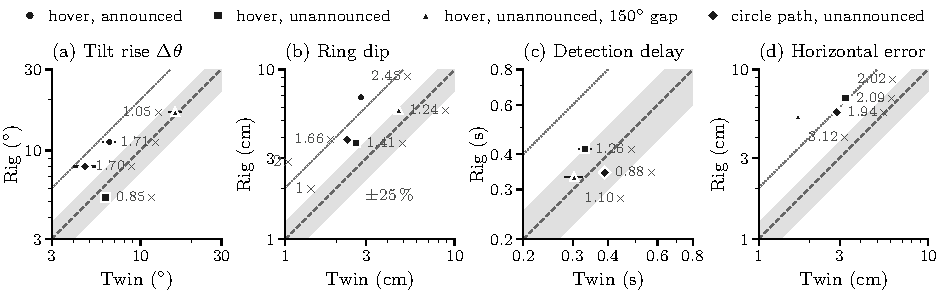
\includegraphics[width=\textwidth]{Images/twin_rig_parity.pdf}
\caption[The twin against the rig]{The rig against its twin for the four releases of 8 October (four UAVs,
0.86\,kg ring at 1.0\,m; one marker per flight; 150$^\circ$ gap: the three left on the ring leave a 150$^\circ$ gap
between two of them), each metric computed the same way from both, on logarithmic axes: $x$, the twin flying the same
configuration (mean of two runs; bar: their range, hidden where it is shorter than the marker); $y$, the rig (one run).
Dashed: $y = x$; grey band: within 25\,\% of the twin; dotted: the rig twice the twin. (a) Tilt rise $\Delta\theta$:
the peak of the ring's tilt-vector departure from its mean over the 5\,s before the release, from the release to the
rig flight's LAND, the twin cut at the same hold. (b) Ring dip: its lowest height error in the 3\,s after the release.
(c) Detection delay: from the release to the planner finding an unannounced release (an announced release needs
none). (d) Horizontal error: the ring's mean distance from its reference over the 10\,s before the release. Within
25\,\% of the twin: the tilt rise of the unannounced hover and 150$^\circ$-gap releases (0.85 and 1.05 times the twin),
the dip of the 150$^\circ$-gap release, and two of the three detection delays (the third is 1.26 times the twin; all
three within 0.1\,s). The announced hover release and the circle release rose 1.7 times the twin; the other three dips
were 1.4--2.5 times the twin's, and the horizontal error was 1.9--3.1 times (5.3--6.8\,cm against 1.7--3.3\,cm).}
\label{fig:twin_rig_parity}
\end{figure}

\paragraph{The carry bands for the next rig day.} The next rig day flies the carriers on 1\,m cables, so the carry
cells were given bands on the 1\,m worlds before it, under a rule signed on 17 October: the band is
$[\max(0, \min - 2\sigma_{\mathrm{rig}}), \max + 2\sigma_{\mathrm{rig}}]$ on the path RMSE and on the peak tilt, from
the path's start to LAND, over three twin runs per cell, with no class factor since no rig carry pair exists on the
current controller, and $\sigma_{\mathrm{rig}}$ from the rig's three-carrier steady hover of 14 October (10.3\,mm on the
path error, 1.50$^\circ$ on the tilt). Because $2\sigma_{\mathrm{rig}}$ is larger than the twin's spread, each band
tests its upper side only: a rig flight misses when its path RMSE exceeds about 30--46\,mm or its peak tilt about
4.6--9.2$^\circ$, depending on the cell (Appendix~\ref{sec:app_bands}).

\paragraph{The pattern so far.} Where the twin and the rig have been compared, on the 8 October releases that
predate the bands, the twin matched the reactive release and missed what it does not model. It has no magnet holding limit: on the layout and pull of L2 its ring peaked at
5.5$^\circ$ (one run) where the rig's capsized. It has no counter-swing: on the rig the survivors' thrust
swung against the step when the plan arrived, in 9 of 9 survivors of the three unannounced 8 October releases
(0.14--1.40\,N at about 1\,Hz). Its ring sits closer
to its reference before a release (1.7--3.3 against 5.3--6.8\,cm). And its rigid rods behave where the rig's tethers
would go slack: the newcomer tipped on 12 of 48 landings after a fold-in in the twin, which the rig's tether should
not do.

\pendingfig{fig:F16}{The ledger: for each rig flight, the band frozen before it (bar) and the rig value (dot), with the
naive predictors.}{the hover and circle releases (L8, L9) and the 1\,m carry cells, from the next rig day}


% drafts_1023.tex -- DRAFTS of 23 Oct 2026, for Wesley's review. Nothing here is reviewed. Index:
% DRAFTS_2026-10-23.md at the worktree root. Removing the one \input line in Results_and_Discussion.tex drops all six;
% each file is a self-contained \subsection with its own labels (sec:res_refly, sec:res_scale, sec:res_rejoin,
% sec:res_catch, sec:res_compare, sec:res_pair_swing), so it can be moved to its place on its own.
% Run ids live only in these comments. Square brackets [ ] mark what is still flying or to be filled.
% Updated 23 Oct afternoon with the day's scored results; res_catch_offset.tex (U) added. A \clearpage after each draft
% flushes its floats before the next one starts (for review; drop them when the sections move to their places).

\noindent\fcolorbox{redoframe}{redoback}{\parbox{\dimexpr\linewidth-2\fboxsep-2\fboxrule\relax}{\small
\textbf{Drafts of 23 October 2026, not reviewed:} the claims on 1\,m cables, scalability, the rejoin of a departed
carrier, the magnet caught off its slot, the comparison with our port of Quan et al.'s method, and the pair's swing on
the rig. Square brackets mark what is still flying.}}

% res_refly_1m.tex -- DRAFT 23 Oct 2026 (thesis result R): every 0.55 m twin table re-flown on 1 m cables.
% Updated 23 Oct afternoon with batch 16 (the five 1 m worlds' tables) and reviewer 2's corrections.
% Sources: card docs/experiments/2026-10-23_refly_1m.md (bars frozen 23 Oct 02:15: each original card's own claim and
% thresholds); docs/analysis/refly_1m_table_2026-10-23.md (tools/refly_score.py, tools/thesis_runsets.py; batch 16 with
% the original cards' own scorers through a scratchpad wrapper); registry R2483-R2577 (1 m, lab PC, 4 slots; W4
% R2483-R2485, Tier A R2486-R2489/R2495-R2498/R2504-R2507, T15 R2490/R2491/R2499/R2500, W5 R2492/R2501, drop
% R2493/R2494/R2502/R2503, T7t R2508-R2537, appendix R2538-R2577); attribution re-flies R2580-R2583 on the same tree at
% 0.55 m; batch 16 R2604-R2628 (Tier B R2604-R2614, the push rows R2615-R2624, gain R2625-R2628; tree be34f95 + patch
% cf1ab9ad, whose only src/ change since R2483-R2577 is the rejoin's fixes, off in every R config).
% Reviewer [weak], 23 Oct 05:15, corrections applied here: C-L2 out of the table (both 1 m L-S runs R2564/R2577 miss S);
% C-D5's mapneg cells out on S and unresolved (footnote c); T7t orbit_v300 attributed by re-fly, not by argument; the
% read-back of R2485, R2521-R2536, R2542-R2550, R2564-R2577 lacks /tracker_2 (registry correction rows).
% Reviewer 2 [weak], 23 Oct 11:47 (Tier B, gain, pushes; every number reproduces to 0.01, all 25 runs valid, no bar
% re-set), corrections applied here: B4 a MARGINAL hold (R2606 0.19 deg under the line, R2612 2.50 under; n = 2, under the
% card's 0.5 deg tilt floor; the tier_b must-not-say stands: nothing says a gap up to 150 deg stays under the line with
% the planned pull); B5 NOT CONFIRMED, not "does not hold" (its falsifier, an abort or fault latch, did not fire); G165's
% drop (R2607/R2613) is an S MISS in both runs (the frozen S exempts only D1/D4/A2/A6; the ">=" reading came after the
% runs); C-D1 vertically and C-D4 EMPTY holds (D-Z0 without the integral already reads 0.06/0.06 cm).
% Tally (refly table doc, 11:47): 19 hold (W4, W5, T3, T8, T9, T15, drop, C-X1, C-X2, C-R1-R4, B1-B4, C-D1, C-D4), 5 do
% not (T7t new; C-L1, C-D2, C-D3, C-D5 as at 0.55 m), 2 unresolved (C-G1, C-G2), 1 not confirmed (B5); 0 void, 0
% skipped. S misses: mapneg R2542/R2549/R2543/R2550 (as at 0.55 m) and G165 R2607/R2613.
% tab:faults' "tilt over 30 deg" row: at 1 m it cites G165 (the integrator's call under Wesley's re-fly-at-1-m decision,
% SESSION_STATE 23 Oct 11:33; he can keep the 0.55 m history instead). tab:faults itself (Appendices.tex) is NOT edited
% here: it still cites the 0.55 m G150p drop.
% NOT REPORTED (Wesley 23 Oct, decisions.md DECIDED 2026-10-23 (9)): the straight-descent landing L-S (C-L2) at 1 m. Its
% two runs stalled 0.14-0.17 m up on the rigid 1 m rods and the stall exit fired; at 0.55 m on this tree it passes
% (R2582/R2583), so the stall is the twin's rigid 1 m rod. (The decision calls it "the 2-quad landing"; the config,
% app_land_straight, has three carriers.)
% The tree changed since the 0.55 m runs (card section 3): land_rearm_touchdown on in the twin (17 Oct); cable_accel_cap
% 12 -> 14.5 m/s^2 (6.6 -> 8 N, 21 Oct); the twin's mocap velocity filter none -> ema (22 Oct); the 1 m defaults (the
% freed UAV's path-clear distance 1.225 m); the 5 s hover hold before every path (T7t's 15 cells, X0-O0/O1). T7t's
% figure-eight is size 0.5 (as flown at 0.55 m; one variable), the rig's is 0.75.
% Must not say (card section 10): no 1 m twin number against a 0.55 m rig flight; "the cable changed X" only with an
% attribution re-fly; W4's 0.55 m column is n = 1; the integral gains are the 0.55 m ones, not re-tuned; the rod error is
% +5 cm absolute (5 % of the rod at 1 m, 9 % at 0.55 m). D-X0's larger steady offset at 1 m (6.6 against 4.8 cm) is not
% put on the cable (no attribution re-fly).

\subsection{The claims on \texorpdfstring{1\,m}{1 m} cables}
\label{sec:res_refly}

This section asks whether the claims that the twin tables of Sections~\ref{sec:res_carry} and~\ref{sec:res_leave}
make on 0.55\,m rods still hold on 1\,m cables, the cables the rig flies from 28 October. Every table was re-flown at
1\,m with its own arms, layouts and repeats, and each claim was scored against its own card's bars, unchanged and
frozen before the re-fly. The baseline is the set of 0.55\,m runs that each table cites. Of the 27 claims scored, 19
hold, 5 do not, 2 stay unresolved as they were at 0.55\,m, and 1 is not confirmed (Tables~\ref{tab:refly_claims},
\ref{tab:refly_steady}, \ref{tab:refly_push} and~\ref{tab:refly_margin}). One of the holds is marginal, and the vertical part of two is
empty: the vertical push left nothing for the remedy to remove.

The comparison is not one variable. Between the 0.55\,m runs and the re-fly the code tree moved: the touchdown test
is re-armed at ring touchdown, the cap on the rod pull that the trackers feed forward was raised, the twin's motion
capture filters velocities as the rig's does, and every path now starts after a 5\,s hover hold. A difference between
the two columns is therefore put on the cable only where the 0.55\,m configuration, re-flown on the new tree,
separates the two (Table~\ref{tab:refly_attrib}). The integral's gains are the ones identified on 0.55\,m rods; they
were not re-tuned for 1\,m. The tables of the release margin, the integral's gain and the constant pushes needed 1\,m
worlds of their own; these were built from the rig's geometry with the cable the only change and flown after the rest,
on the same code but for the rejoin's fixes (Section~\ref{sec:res_rejoin}), which these runs leave off.

\begin{table}[htbp]
  \centering
  \footnotesize
  \setlength{\tabcolsep}{3pt}
  \caption[The twin's claims on 1\,m cables: leaving and carrying]{The release and carry claims of the twin's
  0.55\,m tables, re-flown on 1\,m cables and scored against each card's own bars, frozen before the runs: four UAVs in
  the release rows and three in the carry row, the 0.86\,kg ring at 1.0\,m, floor start, the default controller; runs
  per cell in brackets. The 1\,m runs were flown on one code tree, newer than that of the 0.55\,m runs (see text).
  Release rows: the tilt rise $\Delta\theta$ and the resolution rule of Section~\ref{sec:metrics} (the gap between the
  two arms' means, and the gap the rule needs). $^a$\,With detection off the 1\,m ring peaked lower than the 0.55\,m
  ring, and no 1\,m run ended in an abort in its LAND (0.55\,m: three of three).}
  \label{tab:refly_claims}
  \begin{tabularx}{\textwidth}{>{\raggedright\arraybackslash}p{4.9cm}>{\raggedright\arraybackslash}X>{\raggedright\arraybackslash}X>{\raggedright\arraybackslash}p{1.8cm}}
    \toprule
    Claim (table) & 0.55\,m & 1\,m & At 1\,m \\
    \midrule
    \multicolumn{4}{l}{\emph{Leaving the team}} \\
    The freed UAV is disarmed alone, hover (Table~\ref{tab:T13}) & rest to disarm 0.28\,s; $\Delta\theta$ 6.1$^\circ$ (1)
      & 0.35--0.36\,s; 7.0--7.2$^\circ$ (3) & holds \\ % R1887 | R2483-R2485 (P3 <= 0.003 m, P4 0)
    The freed UAV is disarmed alone, circle (Table~\ref{tab:T13}) & 0.27--0.28\,s; 6.7--7.1$^\circ$ (2)
      & 0.32--0.34\,s; 7.9--8.0$^\circ$ (2) & holds \\ % R1913/R1914 | R2492/R2501
    Pull source, 120$^\circ$ gap: measured $<$ planned (Table~\ref{tab:T9}) & 6.4 against 16.8$^\circ$; gap 10.4, needed 4.4 (3)
      & 7.3 against 17.1$^\circ$; gap 9.8, needed 1.2 (3) & holds \\ % T3: A1 vs A2
    Detection, planner's pull: on $<$ off (Table~\ref{tab:T9}) & 16.8 against 28.2$^\circ$; gap 11.4, needed 1.0 (3)
      & 17.1 against 21.7$^\circ$$^a$; gap 4.6, needed 1.0 (3) & holds \\ % T8: A2 vs A6
    Detection, measured pull: no sign (Table~\ref{tab:T9}) & gap $-$0.8, needed 4.4: unresolved (3)
      & gap $+$0.3, needed 1.4: unresolved (3) & holds \\ % T9: A1 vs A5
    Pull source, 60$^\circ$ circle, no event: planned $<$ measured (Table~\ref{tab:T9}) & 0.53 against 0.93\,cm; gap 0.39, needed 0.30 (2)
      & 0.61 against 0.96\,cm; gap 0.35, needed 0.30 (2) & holds \\ % T15: A8 vs A7
    A second loss, or a 240$^\circ$ gap, drops the ring and lands every UAV (Table~\ref{tab:faults})
      & 4 of 4: dropped 0.22--0.23\,s after the loss; UAV tilt at most 13.6$^\circ$; all down in 8.5--8.9\,s
      & 4 of 4: 0.20--0.22\,s; at most 13.7$^\circ$; 8.1--8.5\,s & holds \\ % D1 R1915/R1916, D4 R1917/R1918 | R2493/R2502, R2494/R2503
    \midrule
    \multicolumn{4}{l}{\emph{Carrying}} \\
    Every cell inside the envelope at 0.55\,m stays inside (Table~\ref{tab:refly_T7t})
      & 14 of 15 cells inside; the spin at 0.3\,m/s outside & 14 of 15 inside; the orbit at 0.3\,m/s outside, the spin
      at 0.3\,m/s inside & does not hold \\
    \bottomrule
  \end{tabularx}
\end{table}

\begin{table}[htbp]
  \centering
  \footnotesize
  \setlength{\tabcolsep}{3pt}
  \caption[The twin's claims on 1\,m cables: steady errors]{The steady-error claims of the twin's 0.55\,m tables,
  re-flown on 1\,m cables as Table~\ref{tab:refly_claims}: three carriers, hover unless stated. $^b$\,A UAV more than
  10\,cm above its rest when the fleet was declared landed; in every case, at both lengths, one UAV was stronger than its
  thrust map; the 1\,m count includes the landings of Table~\ref{tab:refly_push}, all clean. $^c$\,These runs also
  disarm a UAV in the air (footnote~$b$).}
  \label{tab:refly_steady}
  \begin{tabularx}{\textwidth}{>{\raggedright\arraybackslash}p{4.9cm}>{\raggedright\arraybackslash}X>{\raggedright\arraybackslash}X>{\raggedright\arraybackslash}p{1.8cm}}
    \toprule
    Claim (table) & 0.55\,m & 1\,m & At 1\,m \\
    \midrule
    The tracker's relaxed initial condition ($\epsilon = 0.025$) raises the hover by at least 2\,cm (Table~\ref{tab:x0}) & $+$13.1\,cm (2) & $+$18.7\,cm (2) & holds \\ % C-X1
    Pinning the tracker's initial condition ($\epsilon = 0$) at least halves the orbit's error (Table~\ref{tab:x0}) & 0.74 against 3.87\,cm, ratio 0.19 (2)
      & 0.63 against 3.98\,cm, ratio 0.16 (2) & holds \\ % C-X2
    Inside the integral's gate every model error is removed to within 1.0\,cm (Table~\ref{tab:robust})
      & worst 0.87\,cm & worst 0.41\,cm & holds \\ % C-R1
    With the mass typed 20\,\% high, or the rods typed 5\,cm long and not measured, the integral changes the error by
      at most 1.0\,cm (Table~\ref{tab:robust}) & 0.01 and 0.00\,cm; the unmeasured rods leave $+$17.1\,cm
      & 0.01 and 0.00\,cm; $+$17.8\,cm & holds \\ % C-R2: rod+5nomeas +17.09 -> +17.75 both columns
    Measuring the rods absorbs a 5\,cm length error (Table~\ref{tab:robust}) & within 0.00\,cm of the error-free hover
      & within 0.00\,cm & holds \\ % C-R3
    Every robustness flight lands, no UAV past 45$^\circ$ (Table~\ref{tab:robust}) & 28 of 28 & 28 of 28 & holds \\ % C-R4
    The default landing tips no UAV and disarms none in the air$^b$ (Table~\ref{tab:land})
      & no tip; 4 of 82 disarmed in the air, 0.26--0.53\,m up & no tip; 4 of 82 disarmed in the air, 0.17\,m up;
      outward at most 0.8\,cm, tilt at most 5.3$^\circ$ & does not hold, as at 0.55\,m \\ % C-L1: R2542/R2549/R2543/R2550; 68 + the 14 push-arm landings R2615-R2628, all clean
    The model integral removes a thrust-map error's horizontal error better than the target shift
      (Table~\ref{tab:disturbance}) & 0.01 against 0.01\,cm: unresolved (2) & 0.00 against 0.01\,cm: unresolved$^c$ (2)
      & does not hold, as at 0.55\,m \\ % C-D5: D-MM vs D-MR
    \bottomrule
  \end{tabularx}
\end{table}

\begin{table}[htbp]
  \centering
  \footnotesize
  \setlength{\tabcolsep}{3pt}
  \caption[The twin's claims on 1\,m cables: pushes and the integral's gain]{The claims of the twin's 0.55\,m tables on
  a constant push and on the integral's gain, re-flown on 1\,m cables as Table~\ref{tab:refly_claims}, on the 1\,m world
  built for them: three carriers in hover, a 0.6\,N vertical or 0.4\,N horizontal push on the ring for 15\,s. Push
  rows: the steady offset (vertical; horizontal) and the force the integral learned. Gain rows: the peak or the
  overshoot of the vertical push against the default's. $^a$\,Without any integral the vertical push already leaves
  almost no offset (0.06\,cm at 1\,m, at most 0.03\,cm at 0.55\,m): the measured pull takes it up
  (Section~\ref{sec:res_force}), so these vertical holds show nothing.}
  \label{tab:refly_push}
  \begin{tabularx}{\textwidth}{>{\raggedright\arraybackslash}p{4.9cm}>{\raggedright\arraybackslash}X>{\raggedright\arraybackslash}X>{\raggedright\arraybackslash}p{1.8cm}}
    \toprule
    Claim (table) & 0.55\,m & 1\,m & At 1\,m \\
    \midrule
    The model integral removes a constant push to within 1.0\,cm (Table~\ref{tab:disturbance})
      & 0.01--0.02; $-$0.01--0.00\,cm (2) & 0.03--0.06; 0.05\,cm (2) & holds; vertically empty$^a$ \\ % C-D1: D-ZM R2617/R2622, D-XM R2619/R2624
    Without it the push leaves at least 2\,cm (Table~\ref{tab:disturbance})
      & 0.01--0.03; 4.81--4.82\,cm (2) & 0.06; 6.56--6.58\,cm (2) & does not hold vertically, as at 0.55\,m \\ % C-D2: D-Z0 R2615/R2620, D-X0 R2618/R2623
    The integral learns the applied force: 0.45--0.75\,N vertically, 0.30--0.50\,N horizontally (Table~\ref{tab:disturbance})
      & 0.099--0.102; 0.325\,N (2) & 0.112--0.120; 0.325--0.327\,N (2) & does not hold vertically, as at 0.55\,m \\ % C-D3
    The target shift removes the vertical push to within 1.0\,cm (Table~\ref{tab:disturbance})
      & 0.00--0.02\,cm (2) & $-$0.07 to $-$0.06\,cm (2) & holds; empty$^a$ \\ % C-D4: D-ZR R2616/R2621
    Doubling the integral's gain lowers the vertical push's peak (Table~\ref{tab:gain})
      & 1.26--1.44 against 1.25--1.41\,cm: unresolved (2) & 1.42--1.44 against 1.42--1.47\,cm: unresolved (2)
      & unresolved, as at 0.55\,m \\ % C-G1: G-K8 R2625/R2627 vs D-ZM R2617/R2622
    Keeping the speed gate only for 5\,s after the lift lowers the overshoot (Table~\ref{tab:gain})
      & 1.31--1.33 against 1.39\,cm: under the floor (2) & 1.39--1.40 against 1.41--1.44\,cm: under the floor (2)
      & unresolved, as at 0.55\,m \\ % C-G2: G-S5 R2626/R2628 vs D-ZM
    \bottomrule
  \end{tabularx}
\end{table}

The release claims keep their signs at 1\,m. The freed UAV is still disarmed alone, the measured pull still halves the
tilt rise or better at a 120$^\circ$ gap, and a second loss still drops the ring and lands every UAV. With detection
off and the planner's pull, the 1\,m ring rose less than the 0.55\,m ring did and no run ended in an abort, so the
claim holds on a smaller gap. The steady-error claims hold with the same signs: the tracker's relaxed initial condition raises
the hover further on the longer cables, and the unmeasured 5\,cm rod error left the same height error, although the same 5\,cm
is a smaller part of a 1\,m rod. The tables reported without a bar (the hover and paths of Table~\ref{tab:traj}, the
flight of Figure~\ref{fig:flight}) were flown at 1\,m as well, and the landing-lean rows of Table~\ref{tab:T9} were not
re-scored. [Table~\ref{tab:traj} and Figures~\ref{fig:flight}, \ref{fig:traj} and~\ref{fig:detach}: to regenerate from
the 1\,m runs.]
% traj: R2544/R2551 hover 0.03/0.04 cm mean, 0.06 deg (0.55 m 0.04/0.04, 0.06); flight: R2544 (S PASS); K1 not scored.

Four of the five claims that do not hold at 1\,m failed in the same way at 0.55\,m. The landing still disarms the fleet
with a UAV in the air when that UAV is stronger than its thrust map (Section~\ref{sec:sim_landing}); at 1\,m that UAV
was lower when it happened, and the landings of the push rows were all clean. The model integral and the target shift
still leave a thrust-map error's horizontal error equally small, so the integral's advantage there remains unshown.
The vertical push still leaves no offset to remove, so the claims that the push shows without the integral and that
the integral learns its force fail vertically, as they did, and hold horizontally, where the integral removes the
offset and learns the force it learned at 0.55\,m. The integral's gain and its speed gate still make no difference
the resolution rule can resolve. The fifth, the carry envelope, is new at 1\,m.

\subsubsection{The carry envelope at \texorpdfstring{1\,m}{1 m}}

Table~\ref{tab:refly_T7t} gives the carry envelope of Table~\ref{tab:T7t} at both lengths, scored on the clock-free
path error: the rms, over the path, of the ring's distance across the path it was sent and of its height error, with
no schedule in it. The bars are the carry card's: a path error of at most 25\,mm, a peak ring tilt over the path of at
most 6$^\circ$ and a radius ratio of at least 0.95. At 1\,m the orbit at 0.3\,m/s leaves the envelope on two bars at
once, by a small margin on each, and the spin at 0.3\,m/s, outside at 0.55\,m on one run's tilt, comes inside.
Across the envelope the path error rose in every cell but the line's, the radius ratio fell in every cell, and the
path tilt fell or stayed.

\begin{table}[htbp]
\centering
\footnotesize
\setlength{\tabcolsep}{2.6pt}
\caption[The carry envelope on 1\,m cables]{The three-carrier carry envelope in the rig twin on 0.55\,m rods and on
1\,m cables: the 0.86\,kg ring at 1.0\,m, floor start, the default controller, two runs per cell on one code tree per
length (the 1\,m tree is the newer); each cell gives the range over its two runs. Path error: the clock-free path
error (bar 25\,mm); path tilt: the peak ring tilt over the path (bar 6$^\circ$); ratio: the ring's path radius over the
reference's (for the line, the ratio of amplitudes about its centre; bar 0.95). Speed: the peak path speed. Beside
them, not scored: the frozen ring RMSE of Table~\ref{tab:T7t} at 1\,m (its frozen peak tilt was at most 3.0$^\circ$ in
every 1\,m run). $^a$\,Over a bar: the cell is
outside the envelope. $^b$\,Four decimals near the bar.}
\label{tab:refly_T7t}
\begin{tabular}{llcccccc}
\toprule
 & & \multicolumn{2}{c}{Path error (mm)} & \multicolumn{2}{c}{Path tilt ($^\circ$)} & Ratio & Frozen RMSE \\
\cmidrule(lr){3-4}\cmidrule(lr){5-6}
Path & Speed (m/s) & 0.55\,m & 1\,m & 0.55\,m & 1\,m & 1\,m & 1\,m (mm) \\
\midrule
Circle & 0.125 & 2.5 & 3.4--3.5 & 0.86--1.11 & 0.69--0.74 & 0.995 & 9.2--9.8 \\
 & 0.2 & 3.7--6.3 & 7.9--8.1 & 1.45--1.58 & 1.01--1.13 & 0.987--0.988 & 11.7--11.9 \\
 & 0.3 & 11.0--11.7 & 14.7--15.1 & 2.04--2.79 & 1.55--1.60 & 0.975 & 14.9--15.1 \\
\addlinespace
Figure-eight & 0.125 & 3.8--6.8 & 8.1--8.2 & 0.97--1.06 & 0.87--0.91 & 0.987 & 12.0 \\
 & 0.2 & 9.3--10.0 & 14.3--15.0 & 1.48--1.73 & 1.40--1.47 & 0.972--0.974 & 15.5--16.3 \\
 & 0.3 & 15.4--17.6 & 20.5--20.8 & 2.31--2.32 & 2.26--2.33 & 0.955--0.957 & 19.5--19.8 \\
\addlinespace
Line & 0.125 & 1.2--1.4 & 1.1--1.2 & 0.91--0.99 & 0.77--0.79 & 0.990 & 7.8 \\
 & 0.2 & 1.7 & 1.5 & 1.54--1.88 & 1.03--1.18 & 0.973--0.974 & 11.3 \\
 & 0.3 & 2.4--2.6 & 1.5--1.6 & 2.42--2.96 & 2.14--2.18 & 0.951 & 18.0--18.1 \\
\addlinespace
Orbit & 0.125 & 4.1--5.2 & 5.2--5.5 & 0.98--1.07 & 0.75--0.79 & 0.990 & 8.5--8.7 \\
 & 0.2 & 9.0--9.9 & 13.4--13.7 & 1.67--1.88 & 1.09--1.13 & 0.974 & 14.0--14.3 \\
 & 0.3 & 13.2--15.2 & 25.7--25.9$^a$ & 2.49--2.85 & 1.76 & 0.9495--0.9499$^{a,b}$ & 23.8--24.0 \\
\addlinespace
Spin & 0.125 & 2.5--3.5 & 4.5 & 1.05--1.09 & 0.71--0.77 & 0.993--0.994 & 9.5--9.9 \\
 & 0.2 & 3.1--6.0 & 8.2--8.3 & 1.94--2.20 & 1.02--1.15 & 0.987--0.988 & 11.6--12.3 \\
 & 0.3 & 9.0--12.1 & 15.3--15.7 & 3.76--6.31$^a$ & 1.81--1.83 & 0.976 & 15.0--15.5 \\
\bottomrule
\end{tabular}
\end{table}
% 0.55 m: R1847-R1876 (freeze tree, flight code 4b3560e), re-scored on the 22 Oct ruler by tools/refly_score.py (each
% reproduces the carry card's verdicts). 1 m: R2508-R2537 (re-fly tree). R2511 (orbit_v125) is a runner stall 2.4 s
% after LANDED, the flight complete: scored valid (Wesley 23 Oct (4)). Five cells rose more than 1.5x (circle 0.2,
% figure-eight 0.125 and 0.2, orbit 0.3, spin 0.2): informational (card section 5, A), not attributed except orbit 0.3.

The attribution re-fly puts most of the orbit's rise on the code tree, not on the cable
(Table~\ref{tab:refly_attrib}): the same 0.55\,m configuration flown on the new tree already came within a few
millimetres of the bar, and the 1\,m cable added about 2.6\,mm and took the cell over it. Which of the tree's changes
raised the error is not separated. Figure~\ref{fig:refly_orbit} shows where along the orbit the ring runs inside its
path in the three conditions.

\begin{table}[htbp]
\centering
\footnotesize
\caption[Attribution of the orbit's rise]{Attribution of the orbit at 0.3\,m/s, the one cell that leaves the
envelope at 1\,m: the same configuration on 0.55\,m rods flown on the code tree of the 0.55\,m table and on the
re-fly's tree, and the 1\,m cell on the re-fly's tree; two runs each. Bars: path error at most 25\,mm, ratio at least
0.95.}
\label{tab:refly_attrib}
\begin{tabular}{lccc}
\toprule
Cables, code tree & Path error (mm) & Ratio & Path tilt ($^\circ$) \\
\midrule
0.55\,m, the 0.55\,m table's tree & 13.2--15.2 & 0.975--0.977 & 2.49--2.85 \\
0.55\,m, the re-fly's tree & 22.7--23.7 & 0.954--0.956 & 1.75--1.77 \\
1\,m, the re-fly's tree & 25.7--25.9 & 0.9495--0.9499 & 1.76 \\
\bottomrule
\end{tabular}
\end{table}
% R1871/R1872 | R2580/R2581 | R2521/R2536.

\pendingfig{fig:refly_orbit}{The orbit at 0.3\,m/s, the cell that leaves the carry envelope on 1\,m cables: plan view
of the ring's centre over one lap against the reference circle (dotted), on 0.55\,m rods with the 0.55\,m table's code
tree (grey), on 0.55\,m rods with the re-fly's tree (light gold) and on 1\,m cables with the re-fly's tree (gold);
(b) the signed distance across the path along the lap, positive inside, with the tightest quarter shaded.}{the
orbit runs at 0.3\,m/s of the three conditions of Table~\ref{tab:refly_attrib}}
% Data: R1871 (0.55 m, old tree), R2580 (0.55 m, re-fly tree), R2521 (1 m); run.csv payload_x/y and payload_ref_x/y,
% the path from metrics.path_through / project_on_path as tools/n2_bands.path_metrics_clock_free. Tool: a new function
% in tools/thesis_sim_figures.py through the thesis-figure skill.

\subsubsection{The release margin at \texorpdfstring{1\,m}{1 m}}

Table~\ref{tab:refly_margin} gives the margin curve of Table~\ref{tab:T9} on 1\,m cables: a hover release on the
rig's plates that leaves the survivors a gap of 120 to 180$^\circ$, and with it a smaller margin of the ring's centre
of mass inside them. The curve keeps its order: the smaller the margin, the larger the tilt rise, and the measured pull
still rises less than the planner's at 150$^\circ$. Its shape is cleaner at 1\,m, with every step between neighbouring
gaps now resolved with its sign.

Two things changed at the drop line. With the planner's pull at 150$^\circ$ the 1\,m ring no longer reached the
30$^\circ$ line, which it did in both runs at 0.55\,m; one run came within a fraction of a degree of it, so the claim
holds only by its letter, and nothing here says that a gap of up to 150$^\circ$ stays under the line on the planner's
pull. At 165$^\circ$ with the measured pull, under the line at 0.55\,m, the 1\,m ring crossed it in both runs: the
trackers' drop rule dropped the ring and every UAV landed. That is the exit of Table~\ref{tab:faults} working as
built, and at 1\,m these are the runs that stand for its tilt row. The re-fly's safety bar did not allow for a drop
there, so both runs miss it; and in both the freed UAV, already at rest, was disarmed with the fleet when the drop's
landing was declared, not alone. Nothing aborted and no fault fired, which is what that claim's falsifier asks, so it
is not confirmed rather than failed.

\begin{table}[htbp]
  \centering
  \footnotesize
  \setlength{\tabcolsep}{3pt}
  \caption[The release margin on 1\,m cables]{The release-margin claims of the twin's 0.55\,m tables, re-flown on
  1\,m cables and scored as Table~\ref{tab:refly_claims}: four UAVs on the rig's plates, an unannounced hover release
  that leaves the survivors a gap of 120 to 180$^\circ$, the measured pull unless stated; two runs per gap, three at
  120$^\circ$, one for the default rules at 180$^\circ$. Values: the tilt rise $\Delta\theta$ ($^\circ$), the means;
  $\geq$, cut at the drop or the latch. $^a$\,One run came 0.19$^\circ$ under the line, less than the re-fly's
  0.5$^\circ$ floor for a tilt, and its repeat 2.69$^\circ$ under it. $^b$\,Every UAV was disarmed at rest and nothing aborted;
  at 165$^\circ$ the freed UAV was disarmed with the fleet when the drop's landing was declared. $^c$\,A drop the
  re-fly's safety bar did not allow for: both runs miss it.}
  \label{tab:refly_margin}
  \begin{tabularx}{\textwidth}{>{\raggedright\arraybackslash}p{4.9cm}>{\raggedright\arraybackslash}X>{\raggedright\arraybackslash}X>{\raggedright\arraybackslash}p{1.8cm}}
    \toprule
    Claim (table) & 0.55\,m & 1\,m & At 1\,m \\
    \midrule
    A smaller margin gives a larger rise: gaps of 120, 150 and 180$^\circ$, both steps resolved (Table~\ref{tab:T9})
      & 6.4, 16.8 and $\geq$61.2; gaps 10.4 and 44.4, needed 4.4 and 2.0 & 7.3, 17.9 and $\geq$62.2; gaps 10.6 and 44.3,
      needed 1.2 and 1.2 & holds \\ % B1: G120 (A1) / G150 R2605/R2611 / G180 R2608/R2614
    The curve's shape: no step between neighbouring gaps resolved the other way (Table~\ref{tab:T9})
      & 120 to 135$^\circ$ unresolved (gap 2.0, needed 4.4); the rest resolved & every step resolved with its sign
      (120 to 135$^\circ$: gap 3.4, needed 1.2) & holds \\ % B2: G135 R2604/R2610 10.72, G165 R2607/R2613 >= 30.16
    Pull source, 150$^\circ$ gap: measured $<$ planned (Table~\ref{tab:T9}) & 16.8 against $\geq$29.5; gap 12.7, needed 4.3
      & 17.9 against 28.4; gap 10.5, needed 5.0 & holds \\ % B3: G150 vs G150p R2606/R2612
    Every absolute peak under the 30$^\circ$ drop line, gaps 120--150$^\circ$, either pull (Table~\ref{tab:T9})
      & the planner's pull at 150$^\circ$ reached the line in 2 of 2 & largest 29.8$^\circ$, the planner's pull at
      150$^\circ$; no drop$^a$ & holds, marginal \\ % B4: R2606 29.81, R2612 27.31
    Gaps 120--165$^\circ$, the planner's pull at 150$^\circ$ included: no abort, every UAV lands, the freed UAV is
      disarmed alone & 11 of 11; the freed UAV disarmed 0.19--0.43\,s after it came to rest
      & 9 of 11, 0.33--0.37\,s; at 165$^\circ$ disarmed with the fleet$^b$ & not confirmed \\ % B5: G165 0.04 s after LANDED
    \midrule
    \multicolumn{4}{l}{\emph{Reported, no bar (Table~\ref{tab:faults})}} \\
    Ring tilt over 30$^\circ$: the ring dropped, every UAV landed & the planner's pull at 150$^\circ$: 2 of 2
      & the measured pull at 165$^\circ$: 2 of 2, all down in 8.2\,s$^c$; the planner's pull at 150$^\circ$: no drop
      & -- \\ % G165 R2607/R2613 (trackers' 30 deg request +0.50/+0.51 s); 0.55 m G165 landed, abs peaks 28.10/27.84
    A 180$^\circ$ gap with the drop rule off: the fleet disarmed in the air at the 60$^\circ$ latch
      & 1.45--1.62\,m up (2) & 1.84--2.00\,m up (2) & -- \\ % G180 R2608/R2614 (fault at +0.64/+0.65 s)
    The same gap on the default rules: dropped by the gap rule at detection & $\geq$24.1 (1) & $\geq$23.2 (1)
      & -- \\ % G180d R2609 (+0.30 s; 0.55 m +0.32 s)
    \bottomrule
  \end{tabularx}
\end{table}
% Per run (refly table doc, "Batch 16"): G120 R2486/R2495/R2504 6.90/7.45/7.50; G135 10.42/11.02; G150 18.17/17.58;
% G150p 29.62/27.10 (abs 29.81/27.31; back in band 10.11/8.12 s); G165 >=30.49/>=29.84 (abs 30.30/29.57); G180
% >=62.46/>=61.91; G180d >=23.15. A agrees on every arm.

\paragraph{Answer.} On 1\,m cables the twin's claims hold as they did on 0.55\,m rods, with three changes of verdict:
the orbit at 0.3\,m/s now sits just outside the carry envelope, mostly from the code tree and a little from the cable;
the planner's pull at a 150$^\circ$ gap now stays under the drop line, but only just; and at a 165$^\circ$ gap, where
the 1\,m ring now crosses the line and is dropped, the freed UAV is disarmed with the fleet rather than alone. The
claims that failed at 0.55\,m fail the same way at 1\,m, and the gain's two stay unresolved. The 1\,m tables
therefore replace the 0.55\,m twin tables, with this section as the comparison; at 1\,m the drop at 165$^\circ$ stands
for the tilt row of Table~\ref{tab:faults}. The twin's rigid 1\,m rods remain its largest difference from the rig's
slack cables.

\clearpage

% res_scale.tex -- DRAFT 23 Oct 2026 (thesis result S): scalability. Updated 23 Oct afternoon with C, Q6 and Q1-Q5.
% Sources: card docs/experiments/2026-10-23_scalability.md (critic answered 22 Oct; bars FROZEN 23 Oct ~07:25 on Wesley's
% approval, decisions.md DECIDED 2026-10-23 (5): "not so important as long as it works"; eight quads reported "twin
% only, not real time", the real-time limit its own number); its "Results, C" (14:12, lab batch 17, R2700-R2711,
% results/analysis/s_c_twin_2026-10-23.json), "Results, Q6" (14:35, results/analysis/s_quality_bench_n8_2026-10-23.json)
% and "Results, Q1-Q5" (14:58, results/analysis/s_quality_replay_2026-10-23.json); decisions.md DECIDED 2026-10-23 S
% (Wesley ~14:33: N4's window opens 2 s after the last REJOIN_BLEND_OVER for the claim runs; the original window is
% reported beside it) and S's iteration count (~14:37: the 8-quad claims fly at 5 SQP iterations, s8_hover_R50_L100_it5
% and s8_chain4back_R50_L100_it5 x2 each, N1's comparator s4_hover_L100_it5 R2700/R2701; still "twin only, not real
% time"; the it1 8-quad runs stay exploratory). By the card's frozen rule (section 5 B and Q) the rig N_max is read at
% that count too: 5 iterations.
% Bench: registry S-BENCH-1022 (results/analysis/solve_scaling_tuf_2026-10-22.json), S-CALIB-1022
% (s_calib_replay_2026-10-22.json, s_calib_bench_n3_resin/_fast_2026-10-22.json, s_calib_replay_cores_2026-10-22.json;
% rig flights RIG-1022-h3 and -f3h). The bench rows are BEFORE the two speed-ups (plan_fast_refs), the residual inside the
% solve, and no 4 cm pivot in the reference extraction (the pivot adds about 4 ms at n = 3: whole tick p95 32.1 against
% 27.9 ms; 3.5 x 32.1 = 112 ms). Rig-scaled limit: 3.5 x whole tick p95 <= 100 ms, i.e. idle p95 <= 28.6 ms: n = 3 at
% 5 / 2 iterations (27.9 / 18.3 ms; n = 4 48.8 / 29.9), n = 4 at 1 (23.4; n = 5 40.7). Idle limit on latency p95 <= 60
% ms: 4 / 5 / 6.
% Eight-quad exploratory runs (1 iteration): R2464 (s8_hover), R2587 (s8_chain4), R2588 (s8_chain4back before the rejoin
% fixes), R2597 (s8_chain4back on the final rejoin tree).
% Not yet run: bar B (the bench with the speed-ups and the pivot, rig-scaled); the claim cells at 5 iterations (lab batch
% 18: s8_hover_R50_L100_it5 x2, s8_chain4back_R50_L100_it5 x2). NOT written up (Wesley has not decided): the card's
% PROPOSED "More complex cases" addendum (23 Oct ~15:05).
% Open, not in the text: two iterations on the rig (n <= 4 converged by every Q bar) would need a twin closed-loop check
% at it2, the reviewer and Wesley's word (a launch default).

\subsection{Scalability}
\label{sec:res_scale}

This section asks how many UAVs our planner can fly in real time on the rig's laptop, at how few solver iterations
per tick, and whether a larger team can carry a ring down a chain of unannounced releases and back. It gives three
answers apart. The real-time limit comes from a bench calibrated against the rig's own flights. How few iterations
are enough comes from the plans themselves, replayed against converged ones, and from the four-UAV twin flown at one
iteration and at five. The eight-UAV chain is a twin result, flown at a fraction of real time, and says nothing about
real time.

\subsubsection{The real-time limit on the rig laptop}

The planner's tick is one callback of its 100\,ms timer: the solve, the extraction of every UAV's references, and the
dynamics residual that the publish gate reads (Section~\ref{sec:controller}); a tick longer than the period delays
the next. A bench times that tick for a team of $n$ UAVs on the idle laptop, warm-started from its own previous plan
on a figure-eight at 0.2\,m/s and 1\,m cables, for 5, 2 and 1 sequential-quadratic-programming iterations per tick.

The bench is not the rig. Two rig flights of 22 October (three UAVs, five iterations), replayed tick by tick on the
same laptop with nothing else running, took the bench's time; the same ticks in flight took two to three and a half
times as long (Table~\ref{tab:scale_calib}). The factor is therefore the laptop in flight, shared with the rig's stack,
three trackers, motion capture and the recording, and not the flights' states. The limit uses the larger flight's
factor on the 95th percentile, rounded up to 3.5. It is a lower bound for a larger team, which would run more
trackers. One lead, untested on the rig: the laptop has performance and efficiency cores, the replay pinned to an
efficiency core took two and a half times as long as on a performance core, and in flight no tick was as fast as the
performance core's; the planner probably ran partly on the efficiency cores, and the next rig day pins it to the
performance cores.

\begin{table}[htbp]
\centering
\footnotesize
\caption[The bench calibrated against flight]{The planner's solve time on the rig laptop in flight against the same
laptop idle: three UAVs, five iterations, the residual inside the solve; warm ticks only. Replay: the flights' own
ticks solved again on the idle laptop. Bench: the timing bench at three UAVs. The rig factor is the flights' time over
the bench's; the limit of Table~\ref{tab:scale_nmax} uses 3.5 on the 95th percentile (2.1 on the median).}
\label{tab:scale_calib}
\begin{tabularx}{\textwidth}{>{\raggedright\arraybackslash}Xccc}
\toprule
 & Ticks & Median (ms) & 95th percentile (ms) \\
\midrule
Rig laptop in flight, hover & 264 & 36.7 & 67.8 \\
Rig laptop in flight, figure-eight & 573 & 40.4 & 69.4 \\
The same ticks replayed, idle (hover / figure-eight) & 264 / 573 & 18.5 / 19.2 & 19.4 / 20.6 \\
Bench, idle & 200 & 19.8 & 20.1 \\
\addlinespace
Rig factor, both flights pooled & 837 & 1.96 & 3.43 \\
\addlinespace
Hover replayed on one performance / one efficiency core & 264 & 18.4 / 47.7 & 18.9 / 48.9 \\
\midrule
Tick spacing in flight (both flights) & & -- & 116--117$^a$ \\
\bottomrule
\multicolumn{4}{p{0.95\textwidth}}{\footnotesize $^a$\,Measured near each tick's start: 10--12\,\% of ticks more than
110\,ms apart, none more than 150\,ms; the 10\,Hz loop lost no tick.}
\end{tabularx}
\end{table}
% S-CALIB-1022: h3 264 ticks 36.7/67.8 vs replay 18.5/19.4; f3h 573 ticks 40.4/69.4 vs 19.2/20.6; bench n = 3 19.8/20.1;
% k50/k95 1.86/3.37 (h3), 2.04/3.45 (f3h), pooled 1.96/3.43; pinned replay of h3 P-core 18.4/18.9, E-core 47.7/48.9.
% Lower bound: the rig's 60 ms budget cut held 11 (h3) and 37 (f3h) slow ticks to 3-4 iterations.

On that measure the rig laptop flies three UAVs in real time at five or two iterations a tick, and four at one
(Table~\ref{tab:scale_nmax}, Figure~\ref{fig:scale_bench}). The limit is read at five iterations, the count that the
checks of the next part pick: three UAVs. The calibration flights agree: with three UAVs at five iterations the rig's
ticks already came at about its period. The rig has flown four UAVs at five iterations (Section~\ref{sec:res_compute})
because its 60\,ms solve budget cuts the iterations of a slow tick; the limit here is for a tick that finishes its
iterations. The bench with the two speed-ups of the eight-UAV runs and the pivot, which gives the final number, is still
to run.

\begin{table}[htbp]
\centering
\footnotesize
\caption[The real-time limit]{The largest team the planner flies in real time, by solver iterations per tick. Idle:
the bench's latency (the solve and the references' extraction) under 60\,ms at the 95th percentile, the solver's own
throughput. Rig laptop: 3.5 times the bench's whole tick (with the residual) under the 100\,ms period at the 95th
percentile; the limit is read at five iterations. The bench ran before the two speed-ups of the eight-UAV runs and
without the 4\,cm pivot in the extraction, which adds about 4\,ms at three UAVs. No solve failed at any size.}
\label{tab:scale_nmax}
\begin{tabular}{lccc}
\toprule
Iterations per tick & 5 & 2 & 1 \\
\midrule
Idle laptop & 4 & 5 & 6 \\
Rig laptop & 3 & 3 & 4 \\
\addlinespace
Rig laptop, with the speed-ups and the pivot & [\dots] & [\dots] & [\dots] \\
\bottomrule
\end{tabular}
\end{table}
% Last row: the card's bar B (solve_scaling.py --n 2..10 --iters 5 2 1 --fast --pivot-dz 0.04 --rig-factor 3.5
% --tick-budget 100), not yet run (needs the laptop idle with no lab sync). That row is the thesis's number; the S-BENCH
% rows above are its baseline. By the card's rule (section 5: Q and C pick the count; Q6 missed i1 and i2) the rig N_max is
% read at 5 iterations: 3 on the old bench (the morning's "~4 quads" was the 1-iteration column).

\pendingfig{fig:scale_bench}{The planner's whole tick against team size on the idle rig laptop: the 95th percentile
of the solve, the references' extraction and the residual, warm-started, at 5, 2 and 1 iterations per tick (one line
each); dashed: 28.6\,ms, which the rig factor of 3.5 puts at the 100\,ms period in flight; the eight-UAV whole tick of
the twin's hover run, in wall time on the lab computer, for scale.}{the bench with the two speed-ups and the pivot}
% Data: results/analysis/solve_scaling_tuf_2026-10-22.json (now) and the bar-B bench JSON (to run); R2464's planner log
% for the twin point (tick_ms p95 101.2 ms wall). Tool: tools/solve_scaling.py output -> a new thesis_sim_figures
% function through the thesis-figure skill (log y axis; n = 2..9 or 10).

\subsubsection{How few iterations are enough}

Fewer iterations a tick leave the plan short of convergence. Two checks measure what that costs. Replayed tick by
tick, nine recorded flights, five from the twin and four from the rig with two to four UAVs, were solved again at one
and at two iterations from the iterate each tick started from, against the plan converged from the same iterate; an
untimed bench did the same at eight UAVs, with each warm start moved off the plan by about the rig's ring error
(Table~\ref{tab:scale_quality}). And the four-UAV twin flew a hover, the figure-eight at 0.2\,m/s and an unannounced
release at one iteration and at five, each from a floor start (Table~\ref{tab:scale_c}). The bars of both were written
before the runs.

At up to four UAVs, two iterations converge by every bar on all nine flights, the rig's among them. One iteration does
not: on every rig flight, and on the twin's line with a turn of the ring's yaw, its plans break the dynamics by more
than the bar allows. At eight UAVs one iteration misses every bar, and two miss only the thrust feed-forward's,
narrowly. Five pass every bar at eight, so by the rule written before the runs the eight-UAV claims fly at five
iterations, and the real-time limit above is read at five.

\begin{table}[htbp]
\centering
\footnotesize
\setlength{\tabcolsep}{2.5pt}
\caption[The plan at fewer iterations]{The plan at fewer iterations per tick against the plan converged from the same
iterate, replayed tick by tick: nine recorded flights (warm ticks only) and an untimed bench at eight UAVs on the
figure-eight at 0.2\,m/s, each warm start 1\,cm and 10\,cm/s off the plan. 95th percentiles of the dynamics residual (bar $10^{-3}$), of the error of the
references the trackers fly at the next node and the fifth (Ref., bars 5 and 10\,mm), and of the error of the thrust
feed-forward (FF, bar 0.3\,m/s$^2$). Bold: over a bar. The cost's ratio to the converged plan's (bars 1.10 on the median
and 1.50 on the 95th percentile, a tick over the residual bar counted as a miss) failed exactly where the residual did,
and no arm failed a solve. Five iterations at eight UAVs: $3.2 \times 10^{-7}$, 0.9 / 0.9\,mm and 0.12\,m/s$^2$.}
\label{tab:scale_quality}
\begin{tabular}{lcccccc}
\toprule
 & \multicolumn{3}{c}{Two iterations} & \multicolumn{3}{c}{One iteration} \\
\cmidrule(lr){2-4}\cmidrule(lr){5-7}
Flight (UAVs) & Residual & Ref.\ (mm) & FF (m/s$^2$) & Residual & Ref.\ (mm) & FF (m/s$^2$) \\
\midrule
Twin, hover (4) & $1.6{\times}10^{-7}$ & 0.2 / 0.2 & 0.023 & $1.9{\times}10^{-5}$ & 0.3 / 0.5 & 0.036 \\
Twin, figure-eight (4) & $1.3{\times}10^{-7}$ & 0.2 / 0.3 & 0.030 & $1.3{\times}10^{-5}$ & 0.4 / 0.7 & 0.045 \\
Twin, line, yaw turn (4) & $6.1{\times}10^{-6}$ & 0.5 / 0.7 & 0.062 & $\mathbf{2.3{\times}10^{-3}}$ & 1.2 / 2.6 & 0.107 \\
Twin, figure-eight (3) & $2.9{\times}10^{-7}$ & 0.3 / 0.3 & 0.033 & $2.0{\times}10^{-5}$ & 0.4 / 0.7 & 0.050 \\
Twin, figure-eight (2) & $3.1{\times}10^{-7}$ & 0.3 / 0.4 & 0.041 & $4.3{\times}10^{-5}$ & 0.6 / 0.9 & 0.063 \\
\addlinespace
Rig, hover (3) & $6.3{\times}10^{-5}$ & 0.8 / 2.2 & 0.098 & $\mathbf{3.0{\times}10^{-3}}$ & 1.6 / 4.1 & 0.154 \\
Rig, figure-eight (3) & $5.5{\times}10^{-5}$ & 1.3 / 3.0 & 0.144 & $\mathbf{2.3{\times}10^{-3}}$ & 2.3 / 5.6 & 0.227 \\
Rig, line, yaw turn (3) & $1.3{\times}10^{-4}$ & 1.5 / 3.3 & 0.165 & $\mathbf{6.6{\times}10^{-3}}$ & 3.1 / 6.8 & 0.279 \\
Rig, figure-eight (2) & $8.6{\times}10^{-5}$ & 2.2 / 4.6 & 0.247 & $\mathbf{7.4{\times}10^{-3}}$ & 3.7 / 10.0 & \textbf{0.378} \\
\addlinespace
Bench, figure-eight (8) & $8.8{\times}10^{-5}$ & 3.2 / 5.1 & \textbf{0.316} & $\mathbf{9.3{\times}10^{-3}}$ & \textbf{7.3} / \textbf{14.5} & \textbf{0.60} \\
\bottomrule
\end{tabular}
\end{table}
% Q1-Q5: twin R2348 (b4 hover), R2352 (b4 figure-8 size 1.0), R2356 (b4 line_spin, constant-rate turn), R2343 (b3
% figure-8), R2360 (b2 figure-8); rig RIG-1022-h3, -f3h, -ls3c, -f2slope. i1 ticks over the residual bar: R2356 117,
% h3 49, f3h 148, ls3c 232, f2slope 294; i2: f2slope 4. Q6 (n = 8, noise 0.01, untimed): i5 1.000/1.001, 3.2e-7,
% 0.9/0.9, 0.12; i2 1.003/1.010, 8.8e-5, 3.2/5.1, 0.316; i1 170 of 200 ticks over the residual bar. The bench flies
% solve_scaling's figure-8 (size 1.0, 0.2 m/s; --traj-radius 1.0) with a kinematic plant, --noise 0.01 (1 cm, 10 cm/s).

In the twin's closed loop one iteration a tick flew four UAVs as well as five in every cell: inside the carry bands of
the hover and the figure-eight, within the bars set from the five-iteration runs through the lift, the path and the
release, and with no published plan's residual over the bars' limit. It flew the figure-eight a little closer in both repeats, likely because its plan
reached the trackers younger, which was not tested. Its published plans did carry a residual, largest at the release,
that the planner's publish gate never reads at one iteration, since the gate reads it only when the solve budget cuts
a tick; it stayed under the closed loop's limit but over the replay's bar.

\begin{table}[htbp]
\centering
\footnotesize
\setlength{\tabcolsep}{2.4pt}
\caption[Four UAVs at five and at one iteration]{The four-UAV twin at five and at one iteration per tick: the 0.86\,kg
ring at 1.0\,m on 1\,m cables, floor start; hover and the figure-eight (size 1.0 at 0.2\,m/s after a 5\,s hold) on
plates 0, 3, 6 and 9; the release on the join's layout (plates 3, 7 and 11, the UAV on plate 9 released unannounced,
leaving a Y). Two runs each (a / b), one code tree. Path error: the clock-free path error (the hover from 2\,s after
the top to LAND); path tilt peak over the same window, which in the release cell holds the release; lift: from the ring's
reference 1\,cm above its start to 2\,s after the top; release: from the 5\,s mean before it. Residual: the largest
of a published plan, against the closed loop's limit of $10^{-2}$. In brackets, the bars for one iteration, set from
the two runs at five. No run aborted, dropped or failed a solve; the planner flew three UAVs 0.28--0.32\,s after the
release and the ring settled within 0.11$^\circ$ of level.}
\label{tab:scale_c}
\begin{tabular}{llccccc}
\toprule
 & & Path & \multicolumn{3}{c}{Tilt peak ($^\circ$)} & \\
\cmidrule(lr){4-6}
Cell & Iter. & error (mm) & Path & Lift & Release & Residual \\
\midrule
Hover & 5 & 1.34 / 1.32 & 0.25 / 0.20 & 1.77 / 1.87 & -- & $1.1{\times}10^{-8}$ \\
 & 1 & 1.35 / 1.37 [4.33] & 0.24 / 0.21 [1.23] & 1.82 / 1.87 [2.82] & -- & $1.5{\times}10^{-4}$ \\
\addlinespace
Figure-eight & 5 & 11.21 / 11.43 & 1.05 / 1.05 & 1.80 / 1.78 & -- & $1.2{\times}10^{-8}$ \\
 & 1 & 9.66 / 9.84 [14.32] & 0.89 / 0.93 [2.05] & 1.82 / 1.75 [2.79] & -- & $4.2{\times}10^{-4}$ \\
\addlinespace
Release & 5 & -- & 6.75 / 5.79 & 2.57 / 2.54 & 8.25 / 7.40 & $2.5{\times}10^{-7}$ \\
 & 1 & -- & 6.46 / 6.96 [7.27] & 2.63 / 2.66 [3.55] & 8.00 / 8.46 [8.82] & $2.3{\times}10^{-3}$ \\
\bottomrule
\end{tabular}
\end{table}
% R2700/R2701 | R2702/R2703 | R2704/R2705 | R2706/R2707 | R2708/R2709 | R2710/R2711 (lab batch 17, tree be34f95 + patch
% 537551ba, RTF 0.22-0.27, all 12 valid; C1-C7 hold in both repeats of every cell: C CONFIRMS). Closest margins R2711:
% C3 by 0.31 deg, C7's release peak by 0.37 deg. b22 bands: hover <= 22.0 mm / 3.21 deg, figure-8 <= 33.0 / 4.06.
% Published res_eq over 1e-3: 5 ticks in each it1 release run. The it5 pair is also plan_fast_refs' twin smoke run.

One iteration is therefore enough for four UAVs in the twin's closed loop, but its plans are not converged on the
rig's flights and fall short of every bar at eight; two converge for every fleet of up to four, the rig's flights
included.

\subsubsection{Eight UAVs in the twin}

The twin's large ring is 0.5\,m in radius and weighs 0.9\,kg, larger than the rig's ring and not much heavier, with
eight UAVs at 45$^\circ$ on 1\,m cables. The runs flown so far, all exploratory, flew one iteration a tick; the claim
runs fly five. Both fly two changes that shorten the tick without changing its values: every UAV's references come
from one mapped call, and the residual is computed after the references go out. The world runs at a capped fraction
of real time, so a tick that takes the planner its whole period in wall time takes a fraction of it in simulated time:
the result is about the plan and the physics, not about real time, and each run reports its achieved real-time factor
and its late ticks first. Table~\ref{tab:scale_twin} gives the four runs flown so far, one each.

Eight UAVs lifted the ring from the floor and hovered it level. In the chain, every other UAV was released
unannounced, in opposite pairs, so that each release left gaps of at most 90$^\circ$, down to a square of four; the
ring's tilt peaked at a few degrees and the drop rule never fired. In the return, the four freed UAVs, held at
staging points beyond their own plates, rejoined one at a time onto those plates (Section~\ref{sec:res_rejoin}), the
team grew back to eight and landed. Flown again on the final code tree of the rejoin, the chain gave the same
picture (Figure~\ref{fig:scale_chain}). Even in the twin, with the world slowed, the eight-UAV tick at one iteration
took about its whole period of wall time on a 12-core slot of the lab computer, half of it the residual: it is the
whole tick, not the solve, that would overrun first.

The claim runs, two hovers and two chains with the return at five iterations, are still to fly. Their bars were
frozen first, and one has been moved since, still before any claim run flew: the team back at eight is scored from
2\,s after the last rejoin's blend ends, because the rejoin's 10\,s blend, added after the bars were written, put the
last fold-in inside the window first written, from 2\,s after the resize to eight; that window is reported beside it.

\begin{table}[htbp]
\centering
\footnotesize
\setlength{\tabcolsep}{3pt}
\caption[Eight UAVs in the twin]{Eight UAVs in the rig twin, twin only and not real time: the 0.9\,kg ring of radius
0.5\,m at 1.0\,m, eight UAVs at 45$^\circ$ on 1\,m cables, floor start, hover, one iteration per tick; one run each,
exploratory. Releases unannounced, in opposite pairs, down to the square; each rejoin starts 20\,s after the previous
weld and holds the ring through a 10\,s fold-in blend. The first three runs flew before the rejoin's fixes
(Section~\ref{sec:res_rejoin}), the last on its final tree. Ring tilt over the airborne flight. $^a$\,From each
rejoin's start to its rod's end on the plate (before the fixes) or to the weld (final tree); the weld follows the
plate by about 0.1\,s. $^b$\,Ring position error (rms) and tilt peak with the team back at eight, from 2\,s after the
last blend ends to LAND, and in brackets from 2\,s after the resize to eight.}
\label{tab:scale_twin}
\begin{tabularx}{\textwidth}{>{\raggedright\arraybackslash}p{3.0cm}>{\raggedright\arraybackslash}X>{\raggedright\arraybackslash}X>{\centering\arraybackslash}p{1.9cm}c}
\toprule
Run & Releases & Rejoins$^a$ & Ring tilt, median / peak ($^\circ$) & Real-time factor \\
\midrule
Hover & -- & -- & 0.02 / 0.08 & 0.28 \\
8 $\to$ 4 & four, no drop or abort & -- & 0.13 / 3.48 & -- \\
8 $\to$ 4 $\to$ 8, before the fixes & four, no drop or abort & four, 16.1--18.4\,s & 0.18 / 3.25 & 0.2 \\
8 $\to$ 4 $\to$ 8, final tree & four, no drop or abort & four, 15.1--19.4\,s; each rod's end within 1.3--1.6\,cm of
  its plate through the blend; back at eight$^b$ 6.3\,mm, 0.89$^\circ$ (19.3\,mm, 1.65$^\circ$) & 0.52 / 3.35 & -- \\
\addlinespace
Claim cells, five iterations: hover; 8 $\to$ 4 $\to$ 8 & [two runs each, to fly] & [\dots] & [\dots] & [\dots] \\
\midrule
\multicolumn{5}{p{0.93\textwidth}}{Planner tick in the hover run, wall time on the lab computer: solve 44 / 60\,ms
(median / 95th percentile), whole tick 79 / 101\,ms, of which the residual 44--51\,ms; 0.5\,\% of ticks late in
simulated time.} \\
\bottomrule
\end{tabularx}
\end{table}
% R2464 | R2587 | R2588 (wall 28 min, RTF ~0.2) | R2597. Every run landed. R2597's back-at-eight (s_metrics n4 / n4_resize,
% decisions 23 Oct S (1)): revised 6.3 mm / 0.89 deg, original 19.3 mm / 1.65 deg; the bars the 1-iteration claim would
% have had were 5.72 mm / 1.44 deg (N1 from R2702/R2703); the claim runs at 5 iterations take N1 from R2700/R2701. The
% claim cells (N1-N6 of the card): s8_hover_R50_L100_it5 x2, s8_chain4back_R50_L100_it5 x2 (lab batch 18, --slots 2
% --cpus 12 --wall-cap-min 150), scored by tools/s_metrics.py (clock fix of 23 Oct 14:33).

\pendingfig{fig:scale_chain}{Eight UAVs to four and back in the rig twin (twin only, not real time): the 0.9\,kg ring
of radius 0.5\,m, hover, five iterations per tick. (a) The team size the planner flies, with each unannounced release
and each rejoin's start, weld and end of blend marked; (b) the ring's tilt, against the chain's bars of 15$^\circ$ at a
release and 10$^\circ$ at a rejoin; (c) plan views of the formation at eight, at four and back at eight.}{a claim run
of the eight-UAV chain with the return}
% Data: R2597 now (events.csv, run.csv, planner log n), the claim runs later. Tool: tools/s_metrics.py windows -> a new
% thesis_sim_figures function through the thesis-figure skill; panel (c) could be three frames of the run's video
% (results/videos, tools/render_video.py) instead.

\paragraph{Answer.} On the rig laptop our planner flies three UAVs in real time at five iterations a tick, the count
its quality checks pick, on a bench calibrated against the rig's own flights; the final number waits for the bench
with the speed-ups. Fewer iterations are not free: one iteration is enough for four UAVs in the twin's closed
loop, but its plans are not converged on the rig's flights and miss every bar at eight UAVs, while two converge
for every fleet of up to four. In the twin, with the clock taken away, eight UAVs at one iteration carried a larger
ring through four unannounced releases to a square and back to eight, with its tilt peaking at a few degrees, in single
exploratory runs; the claim runs, at five iterations, are to fly. The eight-UAV result is the twin's, and not real
time.

\clearpage

% res_rejoin.tex -- DRAFT 23 Oct 2026: a departed carrier rejoins its own plate (rejoin_departed; twin only).
% Source: card docs/experiments/2026-10-23_rejoin_departed.md (critic 22 Oct answered; E0 bars frozen 23 Oct 00:08, E1
% 00:42, E2-E4 05:13, E5 07:57; critic on the 23 Oct fixes 06:25 "run it", its M2 fixed and M1 logged). Registry: E0 R2445;
% E1 R2457/R2458 (FAIL, 1.5 s blend), R2466/R2467 (VOID as E1b, FAIL as E1), R2578/R2579 (blend fix, PASS), R2592
% (05:59 fixes, PASS), R2596 (hold fix = final tree, PASS); E2 R2584 (FAIL 10.61 deg), R2589 (05:59, PASS), R2594/R2595
% (final, PASS); E3 R2585 (FAIL 1.179 m), R2590 (05:59, PASS); E4 R2586 (FAIL 1.709 m), R2591 (05:59, PASS).
% Code trees: (i) be34f95 + rejoin_blend_s (the rejoin's own 10 s blend); (ii) (i) + the 05:59 fixes (_rejoin_cap,
% REJOIN_OUT_MARGIN_M and the exact way out, the staging bound STAGE_TRACK_M); (iii) (ii) + the path held for
% rejoin_blend_s and the cap's binding logged (the final tree). E3 and E4 flew on (ii): the hold fix acts only through a
% fold-in's blend, which neither reaches (E3 aborts in the descent, E4's ATTACH is refused) -- an inference from the code,
% not a re-fly. E5 (the pair leaning ~3 deg toward / away from the rejoin plate, world three_rigid_ground_rig_T_push_L100,
% Wesley 23 Oct (10); bars frozen 07:57, as E2's): toward R2602 (+3.26 deg at the weld, PASS 3.12 deg) and R2712 (+2.95,
% FAIL 5.28 deg, over 5 from weld +0.22 to +0.41 s: the weld-height cap dipped the rejoiner's reference 1.1 cm, 2.044 ->
% 2.033 m, the critic's M1); away R2603 (-2.67, PASS 2.91) and R2713 (-3.11, PASS 3.37; lean before LAND 1.88 / 1.93
% against 2, the torque on to LAND). Wesley 23 Oct ~14:05: E5 reported as is, 1 of 2 clean toward the plate; no change
% to the cap. Every other E5 bar passes in all four runs.
% Must not say: anything for the rig (the twin's rods are rigid, can push, have no collision geometry, and its joint welds
% at any distance; the rig's magnet catches only on contact, and on the rig the collaborator's controller flies every
% attach). The cap patches a twin mismatch (on a T the rider's rigid rod height IS the ring's pitch), during the blend only.

\subsection{A departed carrier rejoins}
\label{sec:res_rejoin}

This section asks whether a carrier that has left the ring can be flown back to its own plate, re-attached and folded
back into the team, so that the team returns to its size with the ring level. It is the step that closes the chains of
Section~\ref{sec:res_scale}, and it is a twin result only: the twin's joint welds the rod wherever its end is, while
the rig's magnet catches only on contact, and on the rig every attach is flown by the collaborator's controller
(Section~\ref{sec:res_join}). The bars were frozen before each check flew.

\paragraph{How the rejoin flies.} % [Method: move to Section~\ref{sec:reconfig} when this section is placed.]
A freed carrier is not landed. It holds a staging point on its own plate's bearing, 0.3\,m beyond the formation's
reach, which moves and turns with the planned ring and stays inside the position limit. On the operator's ATTACH,
accepted only while the path is held, it flies the newcomer's approach (a climb, a transit over its plate and a
descent at the attach speed), aimed so that its rod's end lands on the plate point it left, with a loop on the
measured end's height. When the end has stayed within 1.5\,cm of the plate point for 0.3\,s and moves slower than
2\,cm/s, the planner asks the twin's joint to weld, waits for the joint to report it, and only then grows its
problem by one UAV, with the remembered plate point and the rod re-measured from the pivot to that point. The fold-in
is the newcomer's: the rejoiner from a vertical rod and a near-zero pull, blended to its share over 10\,s, with the
path held through the blend and the rejoiner's reference held at or below its weld height. A LAND or a drop during a
rejoin sends the rejoiner up, out past the clear radius and down alone.

Table~\ref{tab:rejoin} gives the fold-ins, Table~\ref{tab:rejoin_neighbours} the checks around them. A rejoin is
scored in stages: the rod's end on its plate within 30\,s of the rejoin's start; the joint attached within 0.5\,s of
that; and the fold-in, with the ring's tilt at most 5$^\circ$ from the weld to 15\,s after it, the end within 2\,cm of
its plate through the blend, the rejoiner's planned pull at the blend's end within 10\,\% of its balanced share, the
ring's lean over the last 10\,s before LAND at most 2$^\circ$, and every UAV landed with no drop or abort. Every
neighbouring check passed, and on the final code tree every fold-in but one. The rejoin onto the square (four UAVs back from
three) and onto the T (three back from the opposite pair) both brought the rod's end to its plate inside the 30\,s
allowed, the joint answered within a few hundredths of a second, and the ring stayed well inside its tilt bar through
the fold-in. With the T's pair leaning toward the rejoin plate, one of two fold-ins tipped the ring just past the bar,
briefly; leaning away, both passed, with the ring's lean before LAND the closest to its bar.

\begin{table}[htbp]
\centering
\footnotesize
\setlength{\tabcolsep}{2.4pt}
\caption[A departed carrier rejoins]{A departed carrier rejoins its own plate in the rig twin: the 0.86\,kg ring at
1.0\,m on 1\,m cables, hover, against the bars frozen before the runs (in brackets). Square: the UAV on plate 9 leaves
the square by a ramped release and rejoins it. T: the T's rider (plate 3) is released unannounced, the opposite pair
carries on, and the rider rejoins. Code trees, in order: (i) the rejoin's own 10\,s blend; (ii) with the reference
held at or below its weld height through the blend, the exact way out and the staging bound; (iii) the final tree, with
the path held through the whole blend. Leaning: a steady torque on the ring leans the T's pair about 3$^\circ$ toward
the rejoin plate or away from it. Ranges over $n$ runs. Share: the rejoiner's planned pull at the blend's end against
its balanced share. Lean: the ring's mean tilt over the last 10\,s before LAND (when leaning, with the push still on).
$^a$\,The blend ran for 1.5\,s, not 10\,s (a configuration error, fixed by tree (i)); two more runs with the same short
blend tilted 5.75--5.82$^\circ$. $^b$\,The rejoiner's reference rose 4.6\,cm as the blend swung its rod out, and its
rigid rod lifted the T's free side. $^c$\,5.28$^\circ$ in one run, over the bar for 0.19\,s: at the fold-in the weld-height hold
dipped the rejoiner's reference 1.1\,cm while the pair leaned toward the plate.}
\label{tab:rejoin}
\begin{tabular}{llccccccc}
\toprule
 & & & On its plate & Joint & Ring tilt, weld & End from & & Lean \\
Rejoin & Tree & $n$ & after start (s) & after (s) & to $+$15\,s ($^\circ$) & plate (cm) & Share & ($^\circ$) \\
 & & & [30] & [0.5] & [5] & [2] & [10\,\%] & [2] \\
\midrule
Square & (i) & 2 & 24.86--24.87 & 0.029--0.033 & 1.27--1.30 & 1.3--1.4 & $+$2.5\,\% & 0.08--0.09 \\
 & (ii) & 1 & 24.81 & 0.036 & 1.45 & 1.4 & $+$2.5\,\% & 0.09 \\
 & (iii) & 1 & 23.87 & 0.030 & 1.55 & 1.6 & $+$2.1\,\% & 0.09 \\
T & (ii) & 1 & 17.47 & 0.021 & 3.02 & 1.4 & $-$2\,\% & 0.71 \\
 & (iii) & 2 & 16.58--17.66 & 0.012--0.015 & 1.45--2.25 & 1.3--1.5 & $-$1 to 0\,\% & 0.72--0.79 \\
T, leaning toward & (iii) & 2 & 15.56--16.47 & 0.015--0.018 & 3.12--5.28$^c$ & 1.3--1.5 & $-$1 to 0\,\% & 0.49--0.52 \\
T, leaning away & (iii) & 2 & 17.67--18.56 & 0.015--0.018 & 2.91--3.37 & 1.4--1.5 & $-$1 to 0\,\% & 1.88--1.93 \\
\midrule
\multicolumn{9}{l}{\emph{Before the fixes (failed, kept as results)}} \\
Square$^a$ & -- & 2 & 24.87--25.80 & 0.024--0.027 & 5.32--5.83 & 1.3--1.4 & $-$2\,\% & 0.08--0.09 \\
T & (i) & 1 & 17.47 & 0.021 & 10.61$^b$ & 1.3 & 0\,\% & 0.74 \\
\bottomrule
\end{tabular}
\end{table}
% Square (i) R2578/R2579; (ii) R2592; (iii) R2596. T (ii) R2589; (iii) R2594/R2595. Leaning toward: R2602 / R2712 (lab
% batches 16 / 17; pair lean at the weld +3.26 / +2.95 deg; share +0 / -0.9 %); away: R2603 / R2713 (-2.67 / -3.11 deg;
% -1 / +0.1 %). The cap bound 101 ticks in R2602/R2603, the plan 2.7 / 2.3 cm above it at the last.
% Short blend: R2457/R2458 (scored E1, FAIL); footnote a's two runs R2466/R2467 (VOID as E1b, FAIL as E1 repeats,
% 5.82/5.75 deg).
% T before the fixes: R2584 (tree (i)). Lean column: the registry rows (R2457/R2458 0.09/0.08; R2466/R2467 not recorded
% beyond '<= 2'). Every run landed every UAV, no drop, abort or refusal.

The two failures before the fixes are results. With a 1.5\,s blend the rejoiner took its share almost at once and the
ring tipped just past the bar for a fraction of a second; the full 10\,s blend removed it. On the T the failure was a
twin mismatch: on a T only the rider holds the ring's pitch about the pair's line, and in the twin the rider's rigid
rod makes its height the ring's pitch. As the blend swung the rejoiner's rod out from vertical, its planned height
rose and its rod lifted the T's free side while it carried almost nothing. Holding its reference at or below its weld
height through the blend removed the lift. The hold patches the twin's rigid rod during the blend only; on the rig's
slack tether the mismatch does not arise. Its own small dip at the fold-in, and its release at the blend's end, give
the T's remaining tilt. The hold clamps the reference outside the planner's problem, so its dip is a disturbance of its
own, and it is least sure of itself when the pair leans toward the rejoin plate. Flown with the pair leaning about
3$^\circ$ either way, the fold-ins stayed inside the bar but for one run leaning toward the plate, where the hold's dip
at the fold-in tipped the ring just past it, briefly. That run is reported as it flew; the hold was not changed. With
the pair leaning away, the push that leans it, left on to the end, keeps the ring's lean before LAND close to its bar.

\begin{table}[htbp]
\centering
\footnotesize
\caption[Around the rejoin]{The checks around the rejoin in the rig twin, one run each, against the bars frozen
before the runs. $^a$\,On the floor before the flight the twin's joint welded the rod with its end where it lay, off
the plate; in flight the weld gate prevents this.}
\label{tab:rejoin_neighbours}
\begin{tabularx}{\textwidth}{>{\raggedright\arraybackslash}p{3.4cm}>{\raggedright\arraybackslash}X>{\raggedright\arraybackslash}X>{\raggedright\arraybackslash}p{1.3cm}}
\toprule
Check & Bar & Measured & Verdict \\
\midrule
A rod re-welded on the floor, then the square lifts and hovers (first tree)
  & joint released and re-welded; hover with ring tilt at most 2$^\circ$; every UAV lands
  & both joint states within 0.6\,s; ring tilt 5.6$^\circ$ (median), 6.7$^\circ$ (peak)$^a$; all landed & fails \\
LAND 1.5\,s into the rejoin's descent (tree ii)
  & the rejoin aborts; it climbs until its end is 0.25\,m over its plate before moving out; it lands alone at least
  1.2\,m from the ring centre; no UAV in the air when the fleet is declared landed
  & aborted 0.10\,s after LAND; end 0.27\,m over its plate; landed 1.245\,m out; within 1\,cm of its rest at the
  declaration & passes \\
Staging through a figure-eight lap of the T, with an ATTACH mid-lap (tree ii)
  & the ATTACH refused; the staged UAV inside $\pm$1.6\,m, at least 0.6\,m from the ring centre and 0.8\,m from every
  carrier
  & refused; at most 1.575\,m out along $x$; 0.739\,m from the centre, 1.028\,m from the nearest carrier & passes \\
\midrule
\multicolumn{4}{l}{\emph{Before the fixes (first tree)}} \\
LAND in the descent & as above & landed 1.179\,m out: the way out stopped short & failed \\
Staging on a path & as above & reached 1.709\,m: the staging reference overshot its bound & failed \\
\bottomrule
\end{tabularx}
\end{table}
% E0 R2445 (JOINT_DETACHED 0.004 s after RELEASE, JOINT_ATTACHED 0.58 s after the publish; the re-welded quad sat
% 0.761 m out against 0.733 for its neighbours). E3 R2590 (R2585 before). E4 R2591 (R2586 before); the T's path error in
% the lap 45.5 mm, ring tilt peak 2.74 deg (reported, no bar).

The rejoin also closes the eight-UAV chain of Section~\ref{sec:res_scale}: on the final tree four freed UAVs
rejoined a 0.5\,m ring one at a time, each welded within 20\,s of its start, with every rod's end within 2\,cm of its
plate through its blend (exploratory, one run).

\pendingfig{fig:rejoin}{A freed rider rejoins the T in the rig twin (final code tree, hover, 1\,m cables). (a) The
distance of its rod's end from the plate point it left, against the 1.5\,cm weld gate, with the start, the end on the
plate, the weld and the end of the blend marked; (b) the rejoiner's height reference through the 10\,s blend, with
the cap at its weld height; (c) the ring's tilt against the 5$^\circ$ bar; (d) the rejoiner's planned pull rising to
its share.}{a final-tree rejoin onto the T}
% Data: R2594 (or R2595): run.csv (tether tip poses, payload tilt), the planner log (the rejoiner's reference z and
% planned tension), events.csv (REJOIN_START, REJOIN_ON_PLATE, JOINT_ATTACHED, REJOIN_WELD, REJOIN_BLEND_OVER). Tool: a
% new thesis_sim_figures function through the thesis-figure skill; R2596 (the square) as a second column if it earns it.

\paragraph{Limits.} A rejoin flies only while the path is held; on a path the staged UAV follows its plate and the
ATTACH is refused. The weld waits for the released rod's swing to die by itself: the loop on the measured end trims its
height, not its swing. And the twin flatters the rejoin: its rods are rigid, can push and have no collision geometry,
and its joint welds within the gate wherever the end is.

\paragraph{Answer.} In the twin, a carrier that has left the ring flies back to its own plate, is re-welded and is
folded back in with the ring level, onto a square and onto a T, and the neighbouring checks of a LAND mid-rejoin and of
staging on a path pass. It needed two fixes that the twin's rigid rods and one configuration error forced. With the
T's pair leaning toward the rejoin plate, one fold-in in two went just past the tilt bar, from the dip of the hold that
the rigid rods forced. It is not a rig result.

\clearpage

% res_catch_offset.tex -- DRAFT 23 Oct 2026 (thesis result U): the magnet caught off its slot, twin only.
% Sources: card docs/experiments/2026-10-23_catch_offset.md (critic 23 Oct answered; section 5 FROZEN 07:56 on Wesley's
% four answers, decisions.md DECIDED 2026-10-23 (7): the separation reported apart from the arm comparison (d_sep,
% d_task); t116 a grid cell x2; past ~2.5 cm the claim is worded as a model-error tolerance; the mechanism bar kept);
% its Results (12:41, lab batch 16, R2629-R2684, tools/catch_offset.py as frozen, last edited 00:52); decisions.md
% DECIDED 2026-10-23 "U after batch 16" (Wesley ~14:01): (1) the 6 owed runs fly on today's tree beside batch 16's 54
% counted runs, the table noting both trees; U re-flies whole on the final tree at the results freeze, like R; R2634 is
% a runner race (mocap staleness after /fleet/landed), VOID and re-flown; (2) along the rim the mechanism is NOT SHOWN
% (the scorer's pre-written code), radially in it is shown; the thesis says the slot arm folds in more gently along the
% rim, not that the model point does not matter.
% Runs (repeats a / b). Shared d = 0: measured R2629/R2657, slot R2630/R2658. Along the rim, measured: t02 R2631/R2659,
% t04 R2633/R2661, t06 R2635/R2663, t08 R2637 (VOID: weld 56.3 s after MAGNET ON, 14.3 s before the path)/R2665, t116
% R2639/R2667, t12 R2641/R2669 (R2669 never settled), t16 R2643/R2671 (separation FAIL 0.22/0.23 m). Along the rim, slot:
% t02 R2632/R2660, t04 R2634 (VOID, runner race after LANDED; scorer's code counts it FAIL)/R2662, t06 R2636 (FAIL 1, no
% weld, WELD_TIMEOUT 90 s)/R2664, t08 R2638/R2666, t116 R2640/R2668, t12 R2642/R2670, t16 R2644/R2672 (FAIL 1: weld 68.9 s
% after MAGNET ON; not re-flown). Radially in, measured: ri02 R2645/R2673, ri04 R2647/R2675, ri06 R2649/R2677, ri08
% R2651/R2679, ri12 R2653/R2681, ri16 R2655/R2683; slot: R2646/R2674, R2648/R2676, R2650/R2678, R2652/R2680, R2654/R2682,
% R2656/R2684. Tree be34f95 + patch cf1ab9ad, lab PC, 4 slots, RTF 0.20-0.25, world three_rigid_ground_rig_attach_L100,
% SIM_MOCAP_VEL_FILTER ema. The E-runs R2459-R2463 and the neighbours (u_meas_ta08, u_meas_ro08, u_slot_ro08) are
% exploratory and not in the tables.
% PENDING (owed, 6 runs on today's tree; the lab was taken by another user at ~14:00): re-fly u_meas_t08 (decides the
% falsifier at 8 cm and the measured rim limits: d_tol / d_sep / d_task 8 / 12 / 8, or 6 / 6 / 6); re-fly u_slot_t04
% (the slot rim limits, 4 or 2); u_meas_ri20 x2 and u_slot_ri20 x2 (the pre-registered 20 cm extension radially in).
% Then the reviewer, and U re-flown whole on the final tree.
% Must not say: anything for the rig beyond ~2.5 cm (a real magnet catches only on its 60 mm plate: 16 Oct, three
% slides 3.3-4.3 cm off went past its edge; our contact check confirms within ~24 mm of plate 9); "the model point does
% not matter" along the rim (it matters there, in the slot arm's favour); that the mechanism is shown along the rim; that
% the measured arm's static balance is right at every offset (it is radially in only).

\subsection{The magnet caught off its slot}
\label{sec:res_catch}

This section asks how far off its slot the magnet can catch before the task fails, with the fold-in at the measured
catch point, as the rig folds in, and with the slot assumed instead. It is a twin result. A real magnet catches only on
its 60\,mm plate, and the contact check confirms a catch only within 24\,mm of the plate point
(Table~\ref{tab:constants}); the twin's magnet welds in the air wherever it is told. Up to about 2.5\,cm the sweep is
therefore the rig's case, a real catch error folded in as the rig folds it in. Beyond that it measures the fold-in's
model-error tolerance: how far the attach point the planner is given may lie from the true one before the fold-in
fails, not how far off a real magnet catches. The one real off-slot catch in the sweep is the centre of the next plate
along the rim, 11.6\,cm away: a catch on the wrong plate, which the contact check would refuse on the rig.

\paragraph{How it was flown.} Three carriers on plates 3, 7 and 11 lift the 0.86\,kg ring on 1\,m cables and hold it at
1.0\,m. The newcomer flies this work's own approach to plate 9, which exists only in the twin
(Appendix~\ref{sec:app_proximity_weld}), and the twin's magnet welds its rod's end once it is within 2.5\,cm of the aim
and slower than 0.05\,m/s for 0.15\,s. The aim and the weld point move together by the offset $d$, along the rim
(clockwise, toward the carrier on plate 11) or radially inward, from 0 to 16\,cm. Two arms fold the newcomer in at the
weld: the measured arm at the caught point, as the rig does, and the slot arm at the slot, while the rod pulls from the
caught point, an unmodelled moment that grows with $d$. Both take the caught tip's height, so the arms differ only in
where the planner places the attach point in the ring's plane. The four UAVs then hover, fly one figure-eight
($a = 1.0$\,m) at 0.2\,m/s and land. Two runs per cell, on one host and one code tree.

\paragraph{The bars.} A run fails the task on any of: no weld within 60\,s of the magnet's switch-on, no fold-in within
2\,s of the weld, an abort, a drop, the figure-eight not completed before LAND, or a UAV not landed. The fold-in's bar is
the ring's tilt peak, at most 5$^\circ$ from 1\,s before the weld to 15\,s after it. The arms are compared on
$d_\mathrm{tol}$, the largest offset up to which every cell completed within the bar in both runs. The rule that the
newcomer must stay 0.30\,m from every carrier is scored apart, as $d_\mathrm{sep}$: where the newcomer flies is set by
the arm itself, and the planner has no separation constraint, so crowding is a finding of its own and not a test of
the balance the arms are compared on. The task's limit, $d_\mathrm{task}$, is the smaller of the two. Because equal
limits would show nothing, a mechanism bar asks that the slot arm's excess tilt, at the fold-in or in the steady hover,
grow beyond the repeat spread at $d = 0$ at the two largest offsets both arms flew. All of it was frozen before the
runs.

\begin{table}[htbp]
\centering
\footnotesize
\setlength{\tabcolsep}{3pt}
\caption[The magnet caught off its slot, along the rim]{The magnet caught off its slot along the rim, clockwise toward
the carrier on plate 11, in the rig twin: two runs per cell (a / b). Fold-in: the ring's tilt peak from 1\,s before the
weld to 15\,s after it (bar 5$^\circ$). Steady: the ring's mean tilt in the four-UAV hover, from 15\,s after the weld to
the path. Separation: the newcomer's body to the nearest carrier's, from the weld to LAND (line 0.30\,m). Bold: over the
bar or under the line. Every weld caught within 2.0\,cm of its aim; in every run the tip was within 1\,cm of the aim
19.0--21.1\,s after the magnet's switch-on, and the weld then waited 2.1--48.3\,s for the trigger's speed gate.
$^a$\,Void: a fault of the test runner after the landing (as flown 1.65$^\circ$, 0.62\,m); re-fly owed. $^b$\,No weld
within 60\,s: a task failure. $^c$\,Void: the weld came too late to settle before the path (as flown 2.41$^\circ$,
0.49\,m); re-fly owed. $^d$\,The centre of plate 10: a catch on the wrong plate. $^e$\,This run never settled: the ring
wobbled 3--13$^\circ$ and 6--18\,cm off its reference through the hover and the figure-eight. $^f$\,Welded 68.9\,s after
the switch-on, over the 60\,s allowed: a task failure; its fold-in ran into the path.}
\label{tab:catch_rim}
\begin{tabular}{lcccccc}
\toprule
 & \multicolumn{3}{c}{Measured catch point} & \multicolumn{3}{c}{Slot assumed} \\
\cmidrule(lr){2-4}\cmidrule(lr){5-7}
$d$ (cm) & Fold-in ($^\circ$) & Steady ($^\circ$) & Separation (m) & Fold-in ($^\circ$) & Steady ($^\circ$) & Separation (m) \\
\midrule
0 & 2.21 / 2.02 & 2.29 / 1.93 & 0.65 / 0.65 & 1.58 / 1.70 & 1.02 / 1.46 & 0.65 / 0.65 \\
2 & 1.93 / 1.75 & 2.25 / 1.62 & 0.61 / 0.62 & 1.71 / 1.66 & 1.52 / 1.63 & 0.63 / 0.63 \\
4 & 1.83 / 1.76 & 4.04 / 2.47 & 0.58 / 0.58 & void$^a$ / 1.90 & -- / 2.13 & -- / 0.62 \\
6 & 2.06 / 1.88 & 4.27 / 5.39 & 0.54 / 0.54 & no weld$^b$ / 1.93 & -- / 2.30 & -- / 0.60 \\
8 & void$^c$ / 2.33 & -- / 6.18 & -- / 0.48 & 3.75 / 2.67 & 4.96 / 3.98 & 0.59 / 0.59 \\
11.6$^d$ & \textbf{7.57} / \textbf{7.62} & 5.91 / 6.19 & 0.37 / 0.37 & 3.50 / 3.60 & 4.63 / 5.72 & 0.56 / 0.56 \\
12 & \textbf{5.82} / \textbf{5.14} & 6.36 / 4.93$^e$ & 0.36 / 0.32 & 3.78 / 4.65 & 5.69 / 6.92 & 0.56 / 0.56 \\
16 & \textbf{7.96} / \textbf{8.87} & 7.60 / 5.01 & \textbf{0.22} / \textbf{0.23} & 3.69 / \textbf{7.09}$^f$ & 6.27 / -- & 0.54 / 0.54 \\
\bottomrule
\end{tabular}
\end{table}
% Measured | slot, by d: 0 R2629/R2657 | R2630/R2658; 2 R2631/R2659 | R2632/R2660; 4 R2633/R2661 | R2634/R2662; 6
% R2635/R2663 | R2636/R2664; 8 R2637/R2665 | R2638/R2666; 11.6 R2639/R2667 | R2640/R2668; 12 R2641/R2669 | R2642/R2670;
% 16 R2643/R2671 | R2644/R2672. True offset (cm), measured: 0.7/0.5, 2.3/2.4, 3.8/4.1, 5.9/5.9, 7.8/7.7, 11.5/11.7,
% 12.0/11.9, 15.8/15.7; slot: 1.1/0.1, 2.2/1.7, 4.0/4.0, -/5.5, 8.5/8.1, 11.9/12.0, 12.3/12.6, 15.0/15.9. Model error xy:
% measured 0.1-0.8 cm (the tip's miss of the aim inside the trigger sphere); slot = the true offset. Carrier dip (card
% observation 1, beside the 11.6-16 cm fold-in peaks): slot 36-48 mm (completed runs), measured 85-127 mm. The section 2 static check predicted the
% measured arm's planned body 0.73, 0.67, 0.61, 0.49, 0.36 and 0.23 m from the plate-11 carrier at 0, 2, 4, 8, 12 and 16 cm.

Along the rim the measured arm completed every cell to 6\,cm, and 8\,cm in its one counted run, with its fold-in well
inside the bar (Table~\ref{tab:catch_rim}). From the next plate's centre on, at 11.6, 12 and 16\,cm, its fold-in tilted
the ring past the bar in every run, and at 16\,cm its newcomer came within 0.30\,m of the carrier on plate 11, as the
static check before the runs had predicted. Its steady tilt grew with the offset although its attach point stayed within
a few millimetres of the true one, so the static balance the hypothesis expected at any offset held radially but not
along the rim; why was not separated. The slot arm folds in more gently along the rim: wherever it welded in time its
fold-in stayed under the bar, with a smaller dip of the carriers, and it kept its newcomer near plate 9, clear of the
carriers. Its limit along the rim was set not by the fold-in but by the twin's magnet: at 6\,cm one run never welded,
its tip near the aim but never slow enough for the trigger's speed gate, and at 16\,cm one welded too late and ran into
the path. Those belong to the trigger, which the two arms share until the fold-in, and the rig's magnet has no speed
gate.

\begin{table}[htbp]
\centering
\footnotesize
\setlength{\tabcolsep}{3pt}
\caption[The magnet caught off its slot, radially in]{The magnet caught off its slot radially inward, in the rig twin,
as Table~\ref{tab:catch_rim}. Steady offset: the ring's mean distance from its reference in the four-UAV hover (mm).
Every radial run kept the newcomer at least 0.64\,m from every carrier. The slot arm's newcomer peaked at 0.78--0.79
throttle, against its cap of 0.8, in every radial run with an offset.}
\label{tab:catch_in}
\begin{tabular}{lcccccc}
\toprule
 & \multicolumn{3}{c}{Measured catch point} & \multicolumn{3}{c}{Slot assumed} \\
\cmidrule(lr){2-4}\cmidrule(lr){5-7}
$d$ (cm) & Fold-in ($^\circ$) & Steady ($^\circ$) & Offset (mm) & Fold-in ($^\circ$) & Steady ($^\circ$) & Offset (mm) \\
\midrule
0 & 2.21 / 2.02 & 2.29 / 1.93 & 2 / 1 & 1.58 / 1.70 & 1.02 / 1.46 & 3 / 1 \\
2 & 1.84 / 1.68 & 1.77 / 1.65 & 1 / 1 & 3.23 / 3.29 & 3.82 / 3.98 & 7 / 8 \\
4 & 2.63 / 1.54 & 3.02 / 1.04 & 5 / 2 & 1.83 / 1.81 & 1.31 / 0.99 & 121 / 75 \\
6 & 1.54 / 1.68 & 0.93 / 1.22 & 1 / 1 & 3.45 / 3.27 & 3.15 / 3.05 & 173 / 170 \\
8 & 1.41 / 1.63 & 0.81 / 1.32 & 2 / 1 & \textbf{5.76} / 4.20 & 5.45 / 3.83 & 237 / 192 \\
12 & 1.01 / 1.39 & 0.30 / 1.04 & 3 / 1 & \textbf{10.38} / \textbf{11.71} & 10.44 / 11.91 & 337 / 353 \\
16 & 1.04 / 0.93 & 0.44 / 0.08 & 1 / 3 & \textbf{16.96} / \textbf{14.99} & 16.43 / 15.00 & 396 / 372 \\
\bottomrule
\end{tabular}
\end{table}
% Measured | slot, by d: 0 as along the rim; 2 R2645/R2673 | R2646/R2674; 4 R2647/R2675 | R2648/R2676; 6 R2649/R2677 |
% R2650/R2678; 8 R2651/R2679 | R2652/R2680; 12 R2653/R2681 | R2654/R2682; 16 R2655/R2683 | R2656/R2684. True offset (cm),
% measured: 2.6/2.5, 5.7/3.8, 5.9/6.3, 7.6/8.5, 10.0/12.9, 16.2/14.6; slot: 1.9/2.0, 4.4/3.4, 5.8/5.7, 7.8/6.4,
% 11.4/12.2, 15.4/14.3. Path error after (clock-free figure-8, mm): measured 14.6-17.1; slot 18.4-19.8 at 2 cm, 60.0-90.8
% at 4, 122-124 at 6, 139-168 at 8, 225-238 at 12, 247-265 at 16.

Radially inward the measured arm completed every cell to the largest offset flown, 16\,cm, with its fold-in well inside
the bar and its steady tilt, from 6\,cm on, lower than at $d = 0$ (Table~\ref{tab:catch_in}). The slot arm held the bar
to 6\,cm. From 8\,cm its fold-in tilted the ring past the bar, in one run at 8\,cm and in both beyond, its ring hung
well off its reference in the hover from 4\,cm on, and its newcomer flew near the throttle cap: the unmodelled moment,
as the hypothesis said. Here the attach point matters, and the mechanism bar shows it.

\begin{table}[htbp]
\centering
\footnotesize
\setlength{\tabcolsep}{3pt}
\caption[The catch offset's limits and verdict]{The limits and the verdict of the catch-offset test against its bars,
frozen before the runs. Limits in cm of the nominal offset, with $d_\mathrm{tol}$ on the true offset, run by run, beside
it. In brackets: the value if the void cell's re-fly completes within the bar (and keeps the separation). The
mechanism: the growth of the slot arm's excess tilt over the measured arm's from $d = 0$, against the larger of the two
arms' repeat spreads at $d = 0$ (0.20$^\circ$ at the fold-in, 0.44$^\circ$ steady), at the two largest offsets both arms
flew; the scorer needs two runs a cell, and reads 11.6\,cm where the slot arm's 16\,cm cell has one steady value.}
\label{tab:catch_verdict}
\begin{tabular}{llccccl}
\toprule
Arm & Direction & $d_\mathrm{tol}$ & on the true offset & $d_\mathrm{sep}$ & $d_\mathrm{task}$ & Still to fly \\
\midrule
Measured & along the rim & 6 [8] & 7.7 & 6 [12] & 6 [8] & the 8\,cm re-fly \\
 & radially in & 16 & 16.2 & 16 & 16 & the 20\,cm extension \\
Slot & along the rim & 2 [4] & 5.5 & 2 [4] & 2 [4] & the 4\,cm re-fly \\
 & radially in & 6 & 6.4 & 16 & 6 & the 20\,cm extension \\
\bottomrule
\end{tabular}

\vspace{1ex}
\begin{tabularx}{\textwidth}{>{\raggedright\arraybackslash}p{4.3cm}>{\raggedright\arraybackslash}X>{\raggedright\arraybackslash}p{2.6cm}}
\toprule
Bar & As flown & Verdict \\
\midrule
Confirms: the measured arm's $d_\mathrm{task}$ at least 12\,cm along the rim & 6, at most 8: the fold-in bar from 11.6\,cm
  & not met \\
Confirms: the measured arm's $d_\mathrm{task}$ at least 16\,cm radially in & 16 & met \\
Confirms: the measured arm's $d_\mathrm{tol}$ at least the slot arm's, both directions & along the rim 6 against 2;
  radially 16 against 6 & met; along the rim only through the slot arm's no-weld \\
Confirms: the mechanism shown, both directions & radially: fold-in $+$10.3 and $+$15.5$^\circ$, steady $+$11.4 and
  $+$16.3$^\circ$ at 12 and 16\,cm; along the rim: fold-in $-$0.8 and $-$2.6$^\circ$, steady $+$1.5$^\circ$ at 12\,cm and
  $-$0.01$^\circ$ at 11.6\,cm & radially shown; along the rim not shown \\
Falsifies: the measured arm's $d_\mathrm{task}$ under 8\,cm, either direction & no failure, crowding or tilt over the bar
  at 8\,cm or less (fold-in at most 2.63$^\circ$, separation at least 0.48\,m) & not fired; 8\,cm along the rim has one
  counted run \\
Falsifies: its fold-in over 5$^\circ$ at 4\,cm or less & at most 2.63$^\circ$ & not fired \\
Falsifies: the slot arm's $d_\mathrm{tol}$ over the measured arm's & along the rim 2 against 6; radially 6 against 16
  & not fired \\
\midrule
Overall & & between: neither confirmed nor falsified \\
\bottomrule
\end{tabularx}
\end{table}
% Card Results, "The limits" and "Verdict per frozen bar". Mechanism along the rim by the card's words ("cell mean",
% failed runs included) would read shown (+1.52 at 12 cm, +0.83 at 16 cm on a one-run slot cell); Wesley 23 Oct: the
% scorer's code stands, NOT SHOWN.

Against its bars the result is between: neither confirmed nor falsified (Table~\ref{tab:catch_verdict}). Radially
inward the measured arm reached the 16\,cm asked of it, beat the slot arm, and the mechanism is shown. Along the rim it
fell short of the 12\,cm asked, on the fold-in bar from the next plate's centre on, and the mechanism is not shown: at
the fold-in the slot arm tilted the ring less than the measured arm, and its steady excess did not grow past the repeat
spread at both offsets the scorer read. The measured arm's lead along the rim rests on the slot arm's no-weld at 6\,cm,
which is the trigger's and not the arm's; on the fold-in bar alone the slot arm holds to 12\,cm and the measured arm to
8\,cm. No falsifier fired, though the one at 8\,cm waits for that cell's re-fly.

The twin flatters the attach: its rods are rigid and can push, there is no rotor wash and no contact between rods, and
its magnet welds in the air wherever it is told. At 16\,cm along the rim the newcomer's rod meets the ring about 7\,cm
from the next carrier's, which the rig's rods would not allow.

Six runs are owed and still to fly: a re-fly of each void cell, the measured arm at 8\,cm along the rim, which decides
the falsifier there and the measured arm's limits along the rim, and the slot arm at 4\,cm, which decides the slot
arm's; and the 20\,cm extension radially inward, two runs per arm, pre-registered for a direction in which neither arm
failed by 16\,cm. They fly on a newer code tree than the grid's 54 counted runs, whose flight code differs only in parts
that no run of this test executes; the whole table is re-flown on the final tree before the reviewer sees it.

\pendingfig{fig:catch_offset}{The magnet caught off its slot in the rig twin: the fold-in's ring tilt peak against the
true catch offset, (a) along the rim and (b) radially inward, both arms and both runs of each cell, against the
5$^\circ$ bar, with the 2.5\,cm a real magnet can catch within shaded and the wrong plate's centre marked; (c) along the
rim, the newcomer's closest approach to a carrier against the 0.30\,m line.}{the grid with the two re-flies and the
20\,cm extension}
% Data: tools/catch_offset.py (its JSON for the figure) on R2629-R2684 and the six owed runs. Tool: a new
% thesis_sim_figures function through the thesis-figure skill (Wesley reviews it first).

\paragraph{Answer.} In the twin, with the fold-in at the measured catch point as the rig does it, the task completes
radially inward to the largest offset flown, 16\,cm, and along the rim to 6\,cm, or 8\,cm if that cell's re-fly
completes: from the next plate's centre on, the fold-in tilts the ring past its bar, and at 16\,cm the newcomer crowds
the next carrier. Within the rig's own catch errors, up to about 2.5\,cm, both arms fold in inside the bar. Beyond that
the sweep measures the fold-in's model-error tolerance rather than a real catch: radially the measured point matters,
and with the slot assumed the fold-in fails from 8\,cm; along the rim the mechanism is not shown, and the slot arm folds
in more gently. The result is between, neither confirmed nor falsified, with six runs owed.

\clearpage

% res_compare.tex -- DRAFT 23 Oct 2026 (thesis result C): our planner against our port of Quan et al.'s method, twin.
% Updated 23 Oct afternoon with the search's real best point (lab batch 17).
% Sources: card docs/experiments/2026-10-23_paper_method_compare.md (critic 22 Oct, Response 22 Oct; deviations section
% 3.1; Results scored 14:01 with tools/c_metrics.py); results/analysis/network_tune_search_2026-10-23.json (the offline
% retune); decisions.md DECIDED 2026-10-23 morning (6) (report as is, no harness fix, the card's seven values accepted)
% and late morning (1) (fly the search's real best point, c_net_portfinal: diss_c 12, k_pay = k_anchor 80, k_ring 40,
% k_slot 18, ki_load 0.5, vel_k_att 8, vel_kp_pos 1, vel_kv 3; J 115, every offline guard passes).
% Registry: R2446 (c_net_smoke_hover_L100, as ported), R2447 (c_net_smoke_linex_v200_L100, as ported), R2448
% (c_pl_linex_v400_L100, our planner), R2468/R2469 (c_net_tune_portbest_*: the search's STAGE-1 point, diss_c 12 and
% vel_kp_pos 1 with the rest at the DEFAULTS, flown first in error as "the best"; corrected 23 Oct ~10:00), R2685-R2690
% (c_net_tune_portfinal_*: the search's best, hover / line 0.2 / line 0.4, two each). Our planner's hover: the B baseline
% b4_hover_L100_ema R2348/R2351, scored by tools/c_metrics.py read-only (card section 4; LAND at 40 s cut the 60 s
% window).
% As-ported numbers are the card's Results (c_metrics, in the scored window): yaw largest change 124.7 / 473.7 deg, tilt
% peak 44.81 / 57.67 deg (the registry's whole-run values, yaw range 230 / 602 deg and tilt 44.8 / 67.7 deg, run past the
% loss). Lost runs: their errors are left out of the cell (card section 5).
% PENDING (card Results): our planner's hover x2 (c_pl_hover_L100), line 0.2 x2 (c_pl_linex_v200_L100) and line 0.4 x1
% more (c_pl_linex_v400_L100), so that every case has both arms at n = 2; they wait for the lab (busy since 14:00). The
% paper's form was never flown in the twin. The claim (3 runs per cell on one code tree) was not flown; Wesley: report
% as is, the bars matter less than that it works.
% Must not say: that Quan et al.'s method cannot hold the ring (the capsize comes from our port's yaw-following formation,
% the locked yaw-only design; the paper's payload is a point with no yaw); "dissipative" for our controller.

\subsection{Our planner against our port of Quan et al.'s method}
\label{sec:res_compare}

This section asks how closely our port of Quan et al.'s method \cite{quan2025swarm} carries the ring compared with
our planner. The method holds a team in formation with a virtual spring--damper network and drives each UAV through
a velocity loop; a member leaving or joining needs no new solver, which is why it is the natural comparison for a
team that changes in flight. Both were flown in the rig twin with four UAVs on plates 0, 3, 6 and 9, 1\,m cables and
the ring at 1.0\,m, in hover and on a 0.9\,m line out and back. Up to the hand-over both arms are our planner (the
creep, the lift and a 5\,s hover). After it, our arm keeps our planner and its trackers with the model integral,
while the port's network drives the trackers' velocity loop with no integral per UAV. The comparison is therefore
between the two methods as flown after the lift, not of the network alone. Every run here is exploratory, one or two
per cell (Table~\ref{tab:compare_twin}), and our planner's hover and its line at 0.2\,m/s are still to fly.

\paragraph{The port.} The port follows the authors' description and simulation code where the rig allows, and
departs from the paper in these ways:
\begin{itemize}
  \item \emph{Nodes:} integrated virtual nodes, sprung to a payload node pinned at the target and to an anchor above
  it, as in the authors' simulation code, where the paper's nodes are a kinematic projection.
  \item \emph{Damping:} against the pinned nodes as if they were still, where the paper's friction is relative to the
  formation's centre.
  \item \emph{The command:} our trackers' velocity loop stands in for the authors' autopilot; the thrust feed-forward
  carries a modelled rod pull, not a measured one; the expected acceleration is not fed forward.
  \item \emph{Rod lengths:} at the retuned gains, the rods the planner measured at the hand-over.
  \item \emph{Yaw:} the formation turns with the ring's measured yaw; the paper's payload is a point with no yaw.
  \item \emph{Takeoff:} our planner creeps and lifts; the network takes over 1.5\,s after the lift tops out, seeded at
  the measured UAVs, with its datum moved onto the measured ring.
  \item \emph{Integrators:} one common height trim for the team, none per UAV.
  \item \emph{Plant:} the twin's rigid rods.
\end{itemize}

\paragraph{As ported, the ring capsizes in yaw.} At its first gains the port lost the ring in the twin, in hover and
on the line at 0.2\,m/s: the ring's yaw swung with a growing amplitude until the ring tipped past the abort limits
(Table~\ref{tab:compare_twin}, Figure~\ref{fig:compare_yaw}). The offline harness had predicted this mode: kicked
0.5$^\circ$ in yaw, the ring's yaw grew about one and a half times a second, then it spun and capsized.

\paragraph{Retuned, the port holds the ring but not its yaw.} The retune was set before the comparison flew and
bounded in time: offline, a grid over the network's damping and the velocity loop's position gain, then a descent over
eight gains from the grid's best point, ranked first on guards (no divergence, ring tilt at most 15$^\circ$, UAV tilt at
most 35$^\circ$, throttle at most 0.78, the ring's yaw within 10$^\circ$ and not growing, the hover no worse) and then on
the line's error at 0.4\,m/s (Table~\ref{tab:compare_offline}). The descent's best point passed every offline guard.
Flown in the twin, twice per case, it held the ring in every run, but not its yaw: the ring's yaw swung through tens of
degrees in hover and on the slow line, and least on the fast line, against the guard's 10$^\circ$, and the ring's tilt
peaked well above our planner's. Offline and the twin disagree on the yaw. The harness hangs the
rods from the UAVs' centres and leaves out the 4\,cm pivot below them, which turns a position mismatch into a torque;
that is the likeliest reason it misses the twin's yaw mode, but it was not tested. The paper's own form of the damping
and feed-forward failed only the tilt guard on the 0.6\,m/s line, a speed this comparison does not fly; it is to fly in
the twin.

\paragraph{On the line, a second late and short of the ends.} On the line at 0.4\,m/s the retuned port ran about a
second behind its schedule and turned short of each end, as the harness had predicted. Its error, the distance across
the line plus the shortfall at the ends, was about twice our planner's (Table~\ref{tab:compare_twin},
Figure~\ref{fig:compare_line}). Our planner also turned short of the ends, by less, and ran a few hundredths of a
second late. The error across the line alone would hide the port's shortfall, which is why the comparison adds the
reach. At 0.2\,m/s the port ran later still and turned closer to the ends; our planner's line at that speed is still to
fly.

\begin{table}[htbp]
\centering
\footnotesize
\setlength{\tabcolsep}{2.6pt}
\caption[Our planner against our port in the twin]{Our planner against our port of Quan et al.'s method in the rig
twin: four UAVs on plates 0, 3, 6 and 9, the 0.86\,kg ring at 1.0\,m on 1\,m cables; $n$ runs each, exploratory (our
planner's hover and its line at 0.2\,m/s, and a second run of its line at 0.4\,m/s, are to fly). Both arms are scored
against the target from just before the hand-over. Error: in hover the ring's 3-D error from the hand-over; on the
line the error across the line and in height (clock-free) plus the reach, the shortfall at the line's ends ($+$ short).
Lag: behind the schedule. Yaw: the ring's largest change of yaw in the window. Search's best: the retune's best point
offline, with the measured rods. $^a$\,The four-UAV hover of the baseline set, on a shorter window (LAND at 40\,s). $^b$\,The ring's yaw grew until
it tipped past the abort limits: aborted 27\,s (hover) and 31\,s (line) after the hand-over; the error of a lost run is
not scored.}
\label{tab:compare_twin}
\begin{tabularx}{\textwidth}{>{\raggedright\arraybackslash}p{1.9cm}>{\raggedright\arraybackslash}p{1.3cm}c>{\raggedright\arraybackslash}Xcccccc}
\toprule
 & & & & Error & Clock-free / & Lag & Ring tilt & Yaw \\
Arm & Case & $n$ & Outcome & (mm) & reach (mm) & (s) & peak ($^\circ$) & ($^\circ$) \\
\midrule
Our planner & hover$^a$ & 2 & held & 1.3--1.4 & -- & -- & 0.21 & -- \\
 & hover & [2] & [to fly] & [\dots] & -- & -- & [\dots] & [\dots] \\
 & line, 0.2\,m/s & [2] & [to fly] & [\dots] & [\dots] & [\dots] & [\dots] & [\dots] \\
 & line, 0.4\,m/s & 1 & held & 46.2 & 1.7 / 44.5 & $+$0.03 & 3.5 & 0.2 \\
\addlinespace
Our port, as ported & hover & 1 & capsized$^b$ & -- & -- & -- & 44.8 & 125 \\
 & line, 0.2\,m/s & 1 & capsized$^b$ & -- & -- & -- & 57.7 & 474 \\
\addlinespace
Our port, the search's best & hover & 2 & held & 16.1--18.7 & -- & -- & 8.4--12.9 & 22--51 \\
 & line, 0.2\,m/s & 2 & held & 41.5--42.1 & 9.1--9.9 / 32.2--32.4 & $+$1.25 & 5.0--8.2 & 29--48 \\
 & line, 0.4\,m/s & 2 & held & 99.3--104.5 & 9.3--9.5 / 89.8--95.1 & $+$1.12--1.13 & 11.2--16.4 & 14 \\
\bottomrule
\end{tabularx}
\end{table}
% R2348/R2351 | c_pl_hover_L100 x2 (to fly) | c_pl_linex_v200_L100 x2 (to fly) | R2448 (+ one more to fly) | R2446
% (hand-over 27.47 s, FLEET_ABORT 54.1 s) | R2447 (abort 58.4 s) | R2685/R2686 (first 5 s 22.4/22.5 mm; height -2.9/-3.1
% mm; quad tilt peak 12.9/11.6 deg; throttle peak 0.635/0.615) | R2687/R2688 (reach mean +31.5/+31.2 mm; time-indexed
% error 170.2/170.0 mm; amplitude ratio 0.930/0.931) | R2689/R2690 (reach mean +94.1/+86.3 mm; time-indexed 279.2/278.3
% mm, ours 33.2; amplitude ratio 0.797/0.800; quad tilt 12.0/12.7 deg; throttle 0.624/0.632; path start after the top
% 4.98 s, so net_hold_carry passes) | R2468 (first 5 s 19.0 mm; yaw first over 10 deg at hand-over + 38.9 s; growth
% x1.14/s against x1.43/s as ported) | R2469 (yaw first over 10 deg at + 33.8 s; time-indexed 261.0 mm; amplitude ratio
% 0.712 vs ours 0.909). R2446/R2447 flew with net_twin_geometry off; R2468/R2469 and R2685-R2690 with it on (its own bar
% run was never flown). After LAND the network's quads drop from the cone (quad tilt 174-176 deg): a note only, the
% landings are not compared.

\begin{table}[htbp]
\centering
\footnotesize
\setlength{\tabcolsep}{3pt}
\caption[The port's retune, offline]{The port's retune in the offline harness, not the twin: the
software-in-the-loop plant at the comparison's geometry (the rig's thrust map, the twin UAVs' offsets, the
motion-capture velocity filter), the network at 10\,Hz and the velocity loop at 50\,Hz, started on the taut
60$^\circ$ cone with the ring 0.5$^\circ$ off in yaw, the rods hung from the UAVs' centres. Each point flies hover, the
line at 0.2, 0.4 and 0.6\,m/s and a margin flight (the line at 0.4\,m/s with the velocity loop's gains 1.25 times
higher); the guards are listed in the text. Paper's form: the damping relative to the target's velocity and the
expected acceleration fed forward. Line: as Table~\ref{tab:compare_twin}. Its numbers are not comparable with the
twin's.}
\label{tab:compare_offline}
\begin{tabularx}{\textwidth}{>{\raggedright\arraybackslash}Xcccl}
\toprule
 & Hover & Line 0.4\,m/s: error & Lag & \\
Form and gains & (mm) & (clock-free / reach) (mm) & (s) & Guards failed \\
\midrule
Port, first gains & \multicolumn{3}{c}{capsized 7--15\,s after the start in every case} & all \\
Paper's form, first gains & \multicolumn{3}{c}{capsized 8--16\,s after the start in every case} & all \\
Port, the grid's point: damping doubled, position gain halved & 8.7 & 151.6 (7.2 / 144.4) & $+$1.01 & margin flight; tilt at 0.6\,m/s \\
Port, the search's best (flown in the twin) & 10.2 & 115.1 (6.9 / 108.3) & $+$1.09 & none \\
Paper's form, the search's best & 8.3 & 12.1 (5.3 / 6.7) & $-$0.01 & tilt at 0.6\,m/s \\
\bottomrule
\end{tabularx}
\end{table}
% network_tune_search_2026-10-23.json: port today's diverged hover 15.4, linex 0.2 12.1, 0.4 12.05, 0.6 14.35, margin
% 7.35 s; paper today's 15.4, 16.1, 11.9, 11.4, 7.6 s (the margin flight is the earliest in both forms). Stage-1 point (12, kp 1): J 151.57, guards
% 'linex_v600 ring tilt 15.3 deg', 'margin_linex_v400 diverged at 17.4 s'. Port best J 115.11 (lag 1.087 s): diss_c 12,
% k_pay = k_anchor 80, k_ring 40, k_slot 18, ki_load 0.5, k_att 8, kp_pos 1, kv 3. Paper best J 12.06 (diss_c 3, k_pay 80,
% k_ring 40, k_slot 18, ki_load 0.5, k_att 16, kp_pos 1.5, kv 3), guard 'linex_v600 ring tilt 20.1 deg'. 54 port and 56
% paper candidates; 12 port candidates pass every guard.

The yaw failure belongs to our port. Its formation turns with the ring's measured yaw, a choice made for the ring of
this work, while the paper's payload is a point with no yaw, so these runs say nothing about Quan et al.'s method as
published. Two further twin tests are to fly: the paper's own form of the damping and feed-forward at its best gains, and
the paper's own geometry, with every cable hooked at the ring's centre.
% Wesley 23 Oct: the grid's-point rows (R2468/R2469, flown by an emit error) and the inferred trade-off sentence cut;
% the paper's form (c_net_tune_paperfinal_*) and the centre-hooked geometry to fly (docs/decisions.md).

\pendingfig{fig:compare_yaw}{The ring's yaw after the hand-over in the rig twin, hover, four UAVs on 1\,m cables: our
port as ported (it capsizes, and the run aborts), our port at the search's best gains (the yaw swings but the ring is
held), and our planner (grey; it does not hand over, so its window starts where the port's would).}{the twin hovers of
both arms, our planner's hover cell included}
% Data: R2446, R2685 (or R2686), our planner's c_pl_hover_L100 (to fly; R2348 meanwhile); run.csv ring quaternion ->
% yaw; window from NET_HANDOVER, ours from the top + 1.5 s. Tool: tools/yaw_excursion.py and tools/c_metrics.py windows ->
% a new thesis_sim_figures function through the thesis-figure skill.

\pendingfig{fig:compare_line}{The line at 0.4\,m/s in the rig twin, four UAVs on 1\,m cables, from the path's start:
(a) the ring's position along the line against the schedule (dotted), our planner (gold) and our port at the search's
best gains (blue; about a second late and short of each end); (b) the ring's yaw over the same window.}{the twin line
runs at 0.4\,m/s of both arms}
% Data: R2448 (ours), R2689 or R2690 (the port's best): run.csv payload_x and the reference; PATH_START from events.csv.
% Tool: tools/c_metrics.py windows -> thesis_sim_figures through the thesis-figure skill. Palette: the port is context,
% so grey may suit it better than a colour; the thesis-figure skill decides.

\paragraph{Answer.} In the rig twin our port of Quan et al.'s method as ported capsizes the ring in yaw. At the best
gains of a bounded retune it holds the ring in every run, but not its yaw, which swings most in hover; on the line at
0.4\,m/s its error is about twice our planner's, from running about a second late and turning short of the ends. Our
planner held the ring level and on its path on the fast line; its hover and its slow line are still to fly. The
failure to hold the yaw is our port's, not the published method's.

\clearpage

% res_pair_swing.tex -- DRAFT 23 Oct 2026: the pair's 1.4 Hz swing on the rig (findings; exploratory throughout).
% Sources: rig review docs/reports/rig_review_2026-10-22.md (finding 1, reviewer [weak]: one flight per config, slope
% flights last and h2slope on drained packs, not interleaved); card docs/experiments/2026-10-22_velocity_filter.md (M1:
% the ring normal's horizontal tip band-passed 1.1-1.9 Hz, rms over (a) 0-6 s after lift-off and (b) the hover from the
% top to LAND / drop / detection; tools/pair_swing.py); card docs/experiments/2026-10-23_pair_mode_timing.md (rounds A and
% B, bars frozen 23 Oct 00:42; round C frozen 08:05, R2598-R2601, null; round D reduced, frozen 11:14, R2691-R2694, both
% arms confirm on the thr060 testbed); docs/rig/betaflight_2026-10-22.md (QUAD3
% read-only CLI; ELRS RF mode 8 read as 333 Hz Full from the 14 Oct link statistics: an inference from the mode number).
% Rig rows: RIG-1022-h2, -h2t9p, -h2rts (EMA), -h2slope, -f2slope (slope); -h2m (planned pull) left out (its ring stalled
% 0.37 m short). Twin rows: round A R2449 (cd060 re-fly), R2450/R2451 (thr060), R2452/R2453 (att060), R2454/R2455
% (thr040); round B R2465/R2470 (rt ema 0.55 m), R2471/R2472 (rt slope), R2473/R2474 (rt ema 1 m), R2475/R2476 (rt slope
% 1 m), R2477/R2478 (_rt_norate), R2479/R2480 (_rt050), R2481/R2482 (_rt_nokff). rate_kff 0.027 after the calibration
% run R2456 (0.012) fell outside its band; R2465 is the calibration re-fly, in band at its edge (pitch 35/37 ms).
% Two runner FAILs in round A (R2449, R2453): an envelope fault at touchdown (77.9 deg), after the scored window.
% Decisions 23 Oct late morning: (2) system_overview's latency corrected (done, outside these drafts); (3) round C null,
% round D reduced to the config-only rig candidates on the thr060 testbed; Wed 28's 1 m rig pair is the test; (4)
% rate_kff, thr_tau_s, the body-rate filter emulation and the tip-hinge world DELETED (11:19; backups in the scratchpad's
% del_rt/); the per-channel command delay kept, default off.
% NUMBERS DIFFER (for Wesley): system_overview.tex (i) now gives body rate 17-24 (rig) against 49-57 ms (twin) and
% throttle-to-lift ~15-25 ms in the twin, from the Betaflight note's design numbers; Table pair_timing below gives the
% card's later loop_timing.py readings, 25-35 against 48-62 ms and 17-29 ms. Not edited outside these drafts.

\subsection{The pair's swing on the rig}
\label{sec:res_pair_swing}

This section records a rig finding that the twin does not yet explain. Two UAVs carrying the ring on opposite plates,
the stage that every chain of releases passes through, swing at about 1.4\,Hz on the rig, and the twin's pair does
not. It asks which command path can carry such a swing, and whether a twin given the rig's measured timing reproduces
it. Everything here is exploratory; the first pair on 1\,m cables, on the rig day of 28 October, is the test.

\subsubsection{On the rig}

On 22 October, with the motion-capture velocity filter that was then the rig's default (an exponential moving average),
every two-UAV lift on 0.55\,m rods swung at 1.3--1.6\,Hz, and the swing grew (Table~\ref{tab:pair_rig},
Figure~\ref{fig:pair_rig}). One flight lost the ring when a magnet let go near the top of the lift; the others ended
with the operator's LAND. A higher throttle cap, other plates and references shifted by the plan's age left the swing
as it was. With a filter about 30\,ms faster (the slope of a short window) on the two UAVs the swing halved and
decayed, and the pair carried the ring through a whole figure-eight, the first full lap with two UAVs, with the ring
hanging tilted about the pair's line. Each configuration flew once, and the two slope flights came last, one on drained
packs: the filter is a lead, not a result, until the interleaved repeat of the next rig day.

\begin{table}[htbp]
\centering
\footnotesize
\setlength{\tabcolsep}{3pt}
\caption[The pair on the rig]{Two UAVs carrying the 0.86\,kg ring on opposite plates on the rig, 0.55\,m rods, hover
unless stated, 22 October; one flight each. Velocity filter: the motion-capture velocity estimate the trackers use,
an exponential moving average (about 45\,ms of lag) or the slope of a short window (about 17\,ms). Swing: the rms of
the ring's tip band-passed at 1.1--1.9\,Hz, over the first 6\,s after lift-off (climb) and over the hover. A flight on
the planner's pull, whose ring stalled short of its height, is left out. $^a$\,The flight hovered less than a second.}
\label{tab:pair_rig}
\begin{tabularx}{\textwidth}{c>{\raggedright\arraybackslash}p{1.6cm}>{\raggedright\arraybackslash}p{3.4cm}cc>{\raggedright\arraybackslash}X}
\toprule
 & Velocity & & \multicolumn{2}{c}{Swing ($^\circ$)} & \\
\cmidrule(lr){4-5}
Flight & filter & Change & Climb & Hover & Outcome \\
\midrule
1 & average & plates 0 and 6 & 3.72 & --$^a$ & a magnet let go near the top of the lift (6.4\,N peak pull); ring dropped, every UAV landed \\
2 & average & plates 11 and 5; throttle cap 0.9 & 2.60 & --$^a$ & operator LAND, swing growing \\
3 & average & as 2; references shifted by the plan's age & 2.99 & --$^a$ & operator LAND, swing growing \\
4 & slope & as 2 & 1.46 & 0.79 & swing decaying; landed \\
5 & slope & as 2; figure-eight at 0.2\,m/s & 1.35 & 0.74 & the whole lap; the ring hung about 7$^\circ$ about the pair's line \\
\bottomrule
\end{tabularx}
\end{table}
% 1 RIG-1022-h2 (1.41 Hz; QUAD3's magnet at ring z 0.94 m, lift 95 %; UNANNOUNCED DETACH, DROP AND LAND, ring 62 deg);
% 2 -h2t9p (1.49 Hz; throttle never above 0.77, so the cap was never used; LAND 6.2 s after lift-off); 3 -h2rts (1.45 Hz,
% ref_time_shift on); 4 -h2slope (the 0.71 Hz pendulum left); 5 -f2slope (3-D RMSE 3.7 cm, tilt peak 14.3, mean on the
% path 7.3 deg, lag 0.10 s). Climb values: the velocity-filter reviewer's, reproduced by tools/pair_swing.py within 0.1 deg.

\pendingfig{fig:pair_rig}{The pair's swing on the rig, 22 October: the ring's tip band-passed at 1.1--1.9\,Hz against
time from lift-off, two UAVs on opposite plates, 0.55\,m rods. (a) The three flights with the averaging velocity
filter, the swing growing until LAND or a magnet's release; (b) the two flights with the slope filter, the swing
decaying.}{the five rig flights of Table~\ref{tab:pair_rig}}
% Data: results/rig/2026-10-22/{h2,h2t9p,h2rts,h2slope,f2slope}_logs (ring pose). Tool: tools/pair_swing.py (its
% band-pass and windows) -> a new thesis_rig_figures function through the thesis-figure skill.

\subsubsection{Hardware and timing}

The flight controllers run Betaflight in rate mode: each holds the three body rates it is sent, with a feed-forward on
the rate command and a fast rate loop, and passes the collective throttle to the motors with no loop on it. The tracker
sends its commands at 50\,Hz, the laptop writes the latest frame to each radio every 10\,ms, and the ExpressLRS link
runs at 333\,Hz (inferred from the mode its link statistics report). Radio and flight controller together add only about 10--15\,ms
(Table~\ref{tab:pair_timing}). Measured end to end, the rig differs from the twin per channel: it turns a body-rate
command into body rate faster than the twin, and a throttle command into lift slower, since nothing on the flight
controller closes a loop on thrust and the motors' spin-up shows in full; and the body rate the trackers see lags by
the motion-capture node's own filter. A single command delay in the twin therefore stood for two different things.
No setting of the flight controllers was changed for this work.

\begin{table}[htbp]
\centering
\footnotesize
\caption[The rig's command timing]{The rig's command timing, from the flight controller's configuration (read only)
and the rig's logs of 22 October, against the twin before the timing rounds. Estimates per stage add to the radio and
flight controller's share; the end-to-end paths are measured as an equivalent delay. $^a$\,From the trackers' log
(14--28\,ms from the recordings). $^b$\,The motion-capture node's moving average on the body rates (always on).}
\label{tab:pair_timing}
\begin{tabular}{lcc}
\toprule
 & Rig (ms) & Twin (ms) \\
\midrule
\multicolumn{3}{l}{\emph{Stages, estimated}} \\
Laptop frame hold (a 100\,Hz writer after the 50\,Hz tracker) & 0--10 & -- \\
Radio packet wait and air time at 333\,Hz & 2--3 & -- \\
Command smoothing on the flight controller & 2 (6 at worst) & -- \\
Gyro and rate-loop filters & 1--2 & -- \\
Radio and flight controller together & 10--15 & -- \\
\midrule
\multicolumn{3}{l}{\emph{Paths, measured end to end}} \\
Body-rate command to body rate & 25--35$^a$ & 48--62 \\
Throttle to lift & 44--67 & 17--29 \\
Body rate as the trackers see it$^b$ & 36--48 & 4--5 \\
\bottomrule
\end{tabular}
\end{table}
% Betaflight 4.3.1 (STM32F722), rate profile ACTUAL 100 deg/s linear; rate PID roll P45 I80 D40 F120, pitch P47 I84 D46
% F125, yaw F120; gyro and PID 8 kHz; RC smoothing auto, factor 30; DShot600, airmode; no RPM filter (bidirectional DShot
% off); failsafe: drop after 1.5 s. Twin paths: R2381/R2384/R2385/R2388 after their 60 ms delay was removed (tools/
% loop_timing.py att / lift / filter). QUAD3 read; QUAD1, 2 and 4 assumed the same (not read).

\subsubsection{In the twin}

Four twin rounds asked which path carries the swing, whether the rig's timing or its hinge reproduces it, and what
removes it, each on the twin's pair hover with its delays switched on after the lift (Table~\ref{tab:pair_twin}). In
the first, a 60\,ms delay on every channel made the twin's pair swing; the same delay on the throttle alone swung as
much, and on the body rates alone the pair stayed calm. In the twin, then, the throttle path carries the swing. With
the delay on the body rates alone, though, a slower mode grew until LAND whose shape is the rig's: the ring slid along
the pair's line, and the thrust along the line fed the swing (Figure~\ref{fig:pair_mode}).

In the second round the twin was given the rig's measured timing per channel: the throttle 35\,ms slower, a
feed-forward on the rate loop set so that the body-rate path matches the rig's, and the motion-capture node's filter
on the body rates. It stayed calm with either velocity filter, on 0.55\,m rods and on 1\,m cables, and without the
filter or the feed-forward, which falsifies the reading that the rig's timing alone makes the rig's pair swing. With
the throttle 50\,ms slower it swung, but in the twin's own mode, the UAVs' heights moving with the plates, not in the
rig's. For the first 1\,m pair on the rig the twin therefore predicts no swing with either filter, a weak prediction
from a twin that missed the 0.55\,m pair.

The third round moved the twin's hinge to the magnet tip, 5.75\,cm above the ring's centre of mass as measured on the
rig, with the rig's timing and the planner typed either as on the rig or to the hinge. The pair stayed calm both ways,
so in the twin the hinge's height does not make the rig's swing either. With the second round's reading falsified and
the third null, the rig-timing emulation and the tip-hinge world were removed from the twin; the per-channel delay
stays, off by default, as the instrument of the first and fourth rounds.

The fourth round tried, on the swinging twin, the two changes the rig can fly without new code: the slope filter, and
the trackers on the planner's pull instead of the measured one. Its testbed was the first round's 60\,ms on the
throttle alone. Both removed the swing; on the planner's pull the swing's mode was gone altogether, which places the
twin's swing in the measured pull. The testbed's swing is the twin's own, the UAVs' heights moving with the plates,
not the rig's, so the round shows that each change damps a throttle-delayed swing in the twin, not that either removes
the rig's. The slope filter is already the pair's comparison on the rig on 28 October; the planner's pull would be a
change for the pair alone, since the measured pull is what keeps a release's tilt small (Section~\ref{sec:res_leave}).

\begin{table}[htbp]
\centering
\footnotesize
\setlength{\tabcolsep}{3pt}
\caption[The pair's swing in the twin]{The pair's swing in the rig twin: two UAVs on opposite plates, the 0.86\,kg
ring, hover, 0.55\,m rods unless stated, the averaging velocity filter and the measured pull unless stated; each delay
switched on after the lift. Swing: the hover swing of Table~\ref{tab:pair_rig}; a twin pair counts as swinging at
1.0$^\circ$ or more. Rig timing: the throttle 35\,ms slower, a rate feed-forward matching the rig's body-rate path, and
the motion-capture node's filter on the body rates. Round 3: the rig's timing with the hinge at the magnet tip. Round
4: the first round's 60\,ms on the throttle only, its swing 7.36--7.39$^\circ$ without a change.}
\label{tab:pair_twin}
\begin{tabularx}{\textwidth}{c>{\raggedright\arraybackslash}Xccl}
\toprule
Round & Arm & $n$ & Swing ($^\circ$) & Reading \\
\midrule
1 & 60\,ms on every channel & 1 & 6.95 & swings \\
 & 60\,ms on the throttle only & 2 & 7.36--7.39 & swings as with every channel \\
 & 60\,ms on the body rates only & 2 & 0.56--0.81 & calm; a slower mode grows \\
 & 40\,ms on the throttle only & 2 & 0.10--0.12 & calm \\
\midrule
2 & rig timing & 2 & 0.066--0.081 & calm \\
 & rig timing, slope filter & 2 & 0.029 & calm \\
 & rig timing, 1\,m cables & 2 & 0.065--0.069 & calm \\
 & rig timing, slope filter, 1\,m cables & 2 & 0.029 & calm \\
 & rig timing without the body-rate filter & 2 & 0.077--0.082 & calm \\
 & rig timing without the rate feed-forward & 2 & 0.070--0.089 & calm \\
 & rig timing, the throttle 50\,ms slower & 2 & 4.07--5.14 & swings, in the twin's own mode \\
\midrule
3 & planner typed as on the rig & 2 & 0.08--0.09 & calm \\
 & planner typed to the hinge & 2 & 0.08 & calm \\
\midrule
4 & slope filter & 2 & 0.06--0.07 & calm \\
 & the planner's pull & 2 & 0.01 & calm; no mode at the swing's frequency \\
\bottomrule
\end{tabularx}
\end{table}
% Round A confirms (frozen bars: thr060 >= 0.5x the re-fly, att060 < 0.3x); att060's slower mode 1.0-1.1 Hz, ring slide
% 0.64-0.67 cm/deg, c_u < 0. Round B falsifies (both ema runs < 1 deg and both ring slides < 0.1 cm/deg; items 1, 4, 5
% fail). _rt050 grows to ~19 deg p-p, c_u > 0 (the twin's vertical mode). Checks: att pitch 31-39 ms (rig 25-35).
% Round C (R2598/R2600 typed0175, R2599/R2601 typed0575): the testbed bar fails (typed0175 M1(b) 0.09/0.08 < 1.0 deg;
% ring slide 0.054/0.050 < 0.15): null, no margin claim. Round D (R2691/R2692 slope, R2693/R2694 cable_source model; no-fix
% arm R2450/R2451 7.39/7.36): both arms CONFIRM (both runs <= 3.69 deg, no new fault); D2's f0 1.00 Hz, no 1.5 Hz mode;
% c_u > 0 (the twin's mode). D2 is a candidate for the pair only, after Wed's slope A/B, not a default (the measured pull
% carries Tier A's gains, R1706-R1711). D3-D5 not flown. rate_kff / thr_tau_s / the rate filter / the tip world deleted
% 23 Oct 11:19 (card section 8).

\pendingfig{fig:pair_mode}{The shape of the pair's swing at its frequency, per degree of the ring's see-saw: how far
the ring slides along the pair's line against how far the UAVs' heights move. The rig's flights with the averaging
filter and with the slope filter, against the twin's delayed arms (60\,ms on every channel, on the body rates only)
and the rig-timing twin; the rig's swing slides the ring, the twin's moves the UAVs' heights.}{the rig flights of
Table~\ref{tab:pair_rig} and the twin arms of Table~\ref{tab:pair_twin}, rounds 1--4}
% Data: tools/pair_mode.py on RIG-1022-h2, -h2t9p, -h2rts, -h2slope, -f2slope and on R2381/R2384/R2385/R2388 (cd060),
% R2452/R2453 (att060), R2465/R2470 (rt), R2598-R2601 (round C), R2691-R2694 (round D); slide and dz in cm per deg, c_u as
% the marker's fill (feeds or
% damps). Tool: tools/pair_mode.py -> a new figure function through the thesis-figure skill.

\paragraph{Answer.} The pair's 1.4\,Hz swing is a rig finding. In the twin a delayed throttle carries a swing of the
same frequency, but a twin with the rig's measured timing stays calm, and so does one with the rig's hinge height, so
neither explains the rig's swing. On the twin's own throttle-delayed swing, the faster velocity filter and the
planner's pull each remove it, which says what damps the twin's mode, not the rig's. The faster filter, which calmed
the rig's pair in one flight, waits for its interleaved repeat on the rig, with the first pair on 1\,m cables.

\clearpage
  % DRAFTS 23 Oct (R, S, rejoin, C, pair swing; DRAFTS_2026-10-23.md): delete this line to drop them

% discussion.tex -- Results 4.5: discussion. 17 Oct (v3_full): rewritten in question order on the freeze results;
% skel_discussion merged (feedforward against feedback with the scored 1-DOF signs; the magnet margin; design rules).
% Every number is a result of Sections 4.1-4.4 or of the literature table's sources below.

\subsection{Discussion}
\label{sec:discussion}

This section discusses the answers in question order, then what the twin can and cannot say, the literature, the
design rules that follow and the limitations.

\paragraph{RQ1: carrying on Betaflight with a measured pull.} The cascade carries the ring with all control on the
ground and the UAVs' firmware unchanged: a planner that re-solves the coupled payload--rod problem at 10\,Hz and
trackers that send rate commands over the radio are enough at lab speeds. What limited the carry on the rig was what
the trackers were told about the rods, together with the rod plan: the planned pull assumes massless rods at their planned
angle, and until the trackers used the pull they measure, with the rods planned at 60$^\circ$, the ring lagged its path
and its height swung (Table~\ref{tab:T7}; six settings changed together, and the falsifier that would isolate the
measured pull has not flown). Measuring the rod's pull at each UAV is the ground-side counterpart of the onboard force inversion
of Sun et al.\ \cite{tudelft}, and the rigid-rod twin shows how far it reaches: it takes up a vertical force and an
error in the typed mass at the UAVs themselves (an exploratory one-variable pair separates it), and on the trace one
UAV's thrust-map error, so that the planner's integral, built to remove exactly those, is left with the horizontal axes
and can wind up vertically on an error it cannot see (Section~\ref{sec:res_steady}). The design consequence is that the integral's vertical channel is now a liability as
much as a remedy, and its bound and warning, not its convergence, are what matter there. At speed the ring cuts the
figure-eight's bends by about 3\,cm at 0.3\,m/s; the plan already carries the cut, a timing shift removed it in
exploratory runs, and its source is open (Section~\ref{sec:res_envelope}).

\paragraph{RQ2: geometry first, then the pull source.} Several results that first looked like control
problems are geometry. The twin's tilt rise grows as the support margin shrinks and becomes a loss at zero margin
(Figure~\ref{fig:F12}b); a four-carrier layout can afford at most two particular leavers and never an arbitrary one
(Section~\ref{sec:reconfig}); and every rig release that left an even triangle was carried through. The resize turns
this into an advantage for a centralised controller: the planner knows the whole attachment geometry and solves for
the new shares in the first tick after the event, which statics then fixes, instead of leaving the survivors to find
them from the motion that follows. That supports the working hypothesis of Section~\ref{sec:rq}. What control still
sets after a loss includes when and how the survivors take up the step, and here the one-degree-of-freedom model frozen
before the runs (each survivor's feedforward pull $F = F_{\mathrm{plan}} + k(F_{\mathrm{meas}} - F_{\mathrm{plan}})$, with $k = 0$
on the planner's pull and $k = 1$ on the measured pull) has been scored on the cells flown so far. On an unannounced
release the measured pull gave the smaller tilt rise in both cells flown, as predicted (the sign, not yet the
mechanism, since the two arms started from different states); on the planner's pull, detecting the release cut the tilt rise from 28 to 17$^\circ$,
as predicted; on the measured pull detection made no resolvable difference, as the pure model predicts; and on a
no-event circle the planner's pull tracked better in the twin, as predicted, though narrowly, on the even ring, two runs each
(Section~\ref{sec:res_levers}). The announced half of the crossover, where the plan,
ramped, is predicted to beat the measurement, has not flown, so the design rule stands half-tested: the measured pull
in steady flight and on unannounced events, and the plan, ramped, at announced ones only if that half holds. On the rig
the survivors' thrust swung against the step when the plan arrived, in 9 of 9 survivors of the three unannounced
releases (counter-swing), which the twin does not show and the model has no term for.

\paragraph{The magnet margin.} The binding hardware constraint is the magnet, not the controller. Every ring lost on
the rig began with a magnet letting go: one after a planned tension step of up to 2.75\,N within a second, where the statics asked for 1.61\,N, one in a
steady circle at under a degree of tilt, one in a bobbing lift, and one in a steady hover with a low pack
(Section~\ref{sec:res_detach_rig}). Planning the rods at 60$^\circ$ keeps each pull closer to its plate's axis, but two of
the four losses came after that change, so the plan reduces the risk without removing it, and the drop rule is what
turned the last loss into a controlled landing. The margin a transient leaves is the survivors' peak rod pull and its
rate against the hold at that rod angle (Section~\ref{sec:metrics}); [the hold against the angle of pull is still to
be measured with a spring scale, cold and after the coils have been on for some minutes, on a full and a low pack].

\paragraph{RQ3: a join is an admission, and the rig is limited before it.} Most of the faults that blocked the join
in the twin were in the hand-over between two controllers, not in either controller: a multiplexer that gave
authority to a stream that was armed but idle, a newcomer started with too much tension, a weld gate on the wrong
clock. The contract of Section~\ref{sec:admission} answers that by making every observation this work's own, from
motion capture alone, and the rig confirmed why: its one catch was rejected by a proof that assumed the twin's rigid
tether, and the co-motion confirmation that replaced it, built from the rig's own data, confirms that catch offline.
On the rig the attach is limited earlier, by the magnet reaching the plate at all (Section~\ref{sec:res_join_rig}).
What admission costs the ring waits for the join code tree.

\paragraph{What the resize does not guarantee.} Plug-and-play MPC certifies a change before it is made
\cite{riverso2013plug, zeilinger2013plug}; the resize here is shown, not certified. No solve failed at 26 switches,
each first solve was as converged as the last solve before it, and on the rig the first solve took 24--28\,ms, though 2 of 66 solves in the next second passed the 60\,ms
budget (Section~\ref{sec:res_switch}); but the switch is a change of plant at an instant the planner does not choose,
and the only guard against a first solve that goes wrong is the trackers' envelope and the drop rule.

\paragraph{Simulation and the rig.} The rig twin, flown on the rig's code, matched the reactive release on the four
releases that predate the bands and missed what it does not model: the magnet's hold, the counter-swing, the rig's
offset before a release and the slack tether (Section~\ref{sec:ledger}); no rig flight has yet been scored against a
band frozen before it. Many apparent controller faults in simulation were simulator
artefacts that had to be found and removed before the twin could be trusted: rate estimates differenced from unstamped
poses turned bunched samples into rate spikes under CPU load (the emulated rate loop now uses the gyro); a
proportional-only emulated rate loop could not hold the moment of a rod pivoting below a UAV's centre and flipped UAVs
when control was handed over; the physics engine ignores damping on ball joints, so a damped rod needs universal
joints; and the wall-clock watchdogs fire when the simulation runs slower than real time
(Section~\ref{sec:simulation}). The false touchdown was found the same way, by a twin run that disarmed in the air;
it bears on the rig, because a pack or propeller change can move a UAV's thrust map just as the twin's injected error
did.

\paragraph{Against the literature.} Table~\ref{tab:lit_compare} sets this work against the closest works, in the
numbers each reports. On a path the rig's ring stayed within 3\,cm of its reference on average, 3--5\,\% of the
path's half-extent, the same order as Sun et al.'s 4.1\,\% at 1\,m/s and Wang et al.'s 4.7\,\%; but this work flew at
a tenth of their speed, and the twin's envelope reaches only 0.3\,m/s peak path speed, so the comparison places its accuracy at low
speed only. No work in the table reports a number for the payload's attitude through a departure, or flies a join:
Quan et al.\ release one of four UAVs under a 4\,kg load and report the cable tensions rebalanced after 13\,s, not the
load's attitude. The rig's releases, with tilt rises of 5.3--16.9$^\circ$ over the five carried through, are the only
attitude numbers for a departure in the table; the join has yet to give its number.

\begin{table}[htbp]
\centering
\footnotesize
\setlength{\tabcolsep}{3pt}
\caption{Cooperative transport of a suspended payload: this work against the closest works, as each
reports it. ``--'': not reported.}
\label{tab:lit_compare}
\begin{tabularx}{\textwidth}{@{}
  >{\raggedright\arraybackslash\hsize=0.88\hsize}X
  >{\raggedright\arraybackslash\hsize=0.74\hsize}X
  >{\raggedright\arraybackslash\hsize=0.82\hsize}X
  >{\raggedright\arraybackslash\hsize=1.02\hsize}X
  >{\raggedright\arraybackslash\hsize=1.18\hsize}X
  >{\raggedright\arraybackslash\hsize=0.80\hsize}X
  >{\raggedright\arraybackslash\hsize=1.44\hsize}X
  >{\raggedright\arraybackslash\hsize=1.12\hsize}X@{}}
\toprule
Work & Test; UAVs & Payload; link & Path; speed & Position error\textsuperscript{a} &
Tilt\textsuperscript{b} & UAV removed or added in flight & Control; solve time \\
\midrule
Lee \cite{lee2018geometric},\newline 2018 & Sim; 3 & 1.5\,kg box; rigid links 1\,m &
figure-eight $\pm1.2 \times \pm4.2$\,m; -- & figure only & figure only & -- & geometric PID; -- \\
\addlinespace
Klausen \cite{klausen2020cooperative},\newline 2020 & Real, outdoor; 3 & 1.0, 2.2\,kg point mass; -- &
pilot-set velocity; -- & -- (inter-UAV link error 16--57\,cm) & -- (point mass) & -- &
decentralised passivity-based; -- \\
\addlinespace
Gabellieri\newline \cite{gabellieri2023force}, 2023 & Real (mocap); 2 & 0.2\,kg, 2\,m bar; cables 1\,m &
pose regulation, no path & -- & figure only & -- & decentralised admittance; -- \\
\addlinespace
Wang \cite{wangRobustCooperativeTransportation2024},\newline 2024 & Real (mocap); 3 & point mass; cables
0.6\,m (sim) & curve on a 1.3\,m sphere; 3\,m/s (sim) & mean 6.1\,cm in steady state (4.7\,\%) &
-- (point mass) & -- (cable angle 30 to 70$^\circ$ in flight) & backstepping; -- \\
\addlinespace
Sun \cite{tudelft},\newline 2025 & Real (mocap); 3, some flights 4 & 1.4\,kg; cables 1\,m & figure-eight
$\pm2.5 \times \pm2$\,m; peak 1 to 5\,m/s & RMSE 10.2\,cm (4.1\,\%) at 1\,m/s, 19.7\,cm (7.9\,\%) at
5\,m/s & attitude RMSE 12.9$^\circ$ at 5\,m/s & -- (fixed team) & central OCP 10\,Hz, 2\,s horizon;
mean 15.3\,ms (3 UAVs) \\
\addlinespace
Quan \cite{quan2025swarm},\newline 2025 (preprint) & Real, outdoor; 4 to 6 & 5\,kg; cables 3 to 4.5\,m &
34\,m delivery; -- & -- (sim: 20--68\,\% of the baselines' error) & -- & one UAV released on command (4 to 3, 4\,kg):
tensions rebalanced after 13\,s, attitude --; 94\,\% success over failures and disconnections; joining not flown & decentralised passivity-based; -- \\
\midrule
This work & Real (mocap), twin; 3--4 & 0.86\,kg ring; rigid rods 0.55\,m & circle $r = 0.5$\,m,
0.125\,m/s; figure-eight $\pm1.0 \times \pm0.5$\,m, peak 0.25\,m/s & circle: mean 2.6\,cm (5.2\,\%), max 5.5\,cm;
figure-eight: mean 2.9\,cm (2.9\,\%), max 6.6\,cm & circle 1.7 / 4.0$^\circ$, figure-eight 2.6 / 5.9$^\circ$ (mean /
max) & removed, 4 to 3: tilt rise 5.3--16.9$^\circ$ over five rig releases, loss found in 0.33--0.42\,s; added: [join
tree] & central OCP 10\,Hz, 2\,s; MPC per UAV; median 31--66\,ms \\
\bottomrule
\end{tabularx}

\smallskip
\parbox{\textwidth}{\scriptsize\raggedright
\textsuperscript{a}\,In brackets: the error divided by the path's half-extent along its longer axis
(circle: radius; figure-eight: long semi-amplitude; Wang: sphere radius). This work: mean horizontal
distance from the time-indexed reference (the lag is in it); Sun et al.: 3-D RMSE; Wang et al.:
steady-state mean of the 3-D error. A mean is never larger than the RMSE of the same signal.
\textsuperscript{b}\,Payload tilt. This work: the ring's tilt from level; Sun et al.: axis-angle attitude
error, yaw included. Mocap: motion capture; sim: simulation.
This work's tilt is from the day's analysis of each flight; its path errors are on the reviewed window of
Table~\ref{tab:T7}. Not like-for-like: speed (this work 0.125--0.25\,m/s, Sun et al.\ 1--5\,m/s, Wang et al.\ 3\,m/s in
simulation, not restated for the flight); this work hangs the payload on rigid rods, the others on
cables (Lee: rigid links, simulation only); a point mass (Klausen et al., Wang et al.) has no attitude;
this work's rig entries are one flight each; this work's solve times are
wall-clock medians on a laptop shared with the motion capture and radio nodes, Sun et al.'s a mean CPU
time; Klausen et al.\ and Quan et al.\ fly outdoors on satellite and onboard sensing.}
\end{table}
% ---------------------------------------------------------------------------------------------------
% SOURCES: every number in Table tab:lit_compare. 17 Oct (v3): this work's path errors are now on the T7 window
% (reviewer 12 Oct): circle 2.6 / 5.5 cm (5.2 %), figure-eight 2.9 / 6.6 cm (2.9 %); the lines below keep the 10 Oct registry reading.
% Page references: "p.N" is the printed page; "PDF N" the page index of the file in
% docs/papers/ (multi_drone_control repo). "[computed]" = arithmetic on stated numbers, done here.
%
% Normalisation used for the bracketed % (footnote a): error / half-extent of the path along its longer
% axis. Sun: 2.5 m (x semi-amplitude, Table S1); Wang: 1.3 m (sphere radius, eq. 39); this work: circle
% radius 0.5 m, figure-eight a = 1.0 m (Gerono lemniscate dx = a sin(th), dy = (a/2) sin(2 th), so
% +-1.0 x +-0.5 m; mpc_planner/load_trajectory.py, thesis trajectories.tex).
%
% --- Lee 2018, IEEE TCST 26(1) 255-264, doi 10.1109/TCST.2017.2656060 (file "PDF.js viewer.pdf") ---
%   Simulation only: abstract p.255/PDF 1 "illustrated by a numerical example"; no experiment.
%   n = 3; m0 = 1.5 kg box 1.0 x 0.8 x 0.2 m; m_i = 0.755 kg; l_i = 1 m: p.260/PDF 6, Sec. V.
%   Rigid massless links: abstract ("via rigid links"), Sec. II p.256/PDF 2, Fig. 1 caption.
%   Path x0d = [1.2 sin(0.2 pi t), 4.2 cos(0.1 pi t), -0.5]: p.260/PDF 6. Speed not stated
%   ([computed] peak ~1.5 m/s, not used in the table).
%   Position and attitude error: Fig. 2(a), 2(b) only (Psi0 = 1/2 ||R0 - R0d||^2); no number in the text.
%   No UAV removal/addition; no control rate or computation time.
%
% --- Klausen et al. 2020, IEEE TCST 28(2) 653-660, doi 10.1109/TCST.2018.2876518 (cooperative_control.pdf) ---
%   Real: three hexacopters "each weighing 2.3-kg" (p.653/PDF 1; also m_c = 2.3 kg p.657/PDF 5; p.658
%   says "2.2-kg UAVs": inconsistent in the paper, 2.3 used here). Loads "approximately 1 kg" and
%   "approximately 2.2 kg" (p.657/PDF 5); point-mass load model. Outdoor, GNSS RTK + IMU (p.653, p.657).
%   Formation "equal-sided triangle with sides of 5 m" (p.657/PDF 5); velocity reference set by a
%   pilot (p.657, p.659). Cable length for the flights: not stated (simulation: l_i = 2 m, p.656/PDF 4).
%   Mean link error (inter-UAV distance error, NOT payload error), Table I p.659/PDF 7: light load
%   0.38 / 0.37 / 0.16 m, heavy load 0.57 / 0.34 / 0.46 m -> "16-57 cm" in the table.
%   Simulation (p.656/PDF 4): N = 3, UAV 2 kg, load 3 kg, wires 2 m, 1 m/s, wind 4 m/s; link error
%   plotted only (Fig. 5). Wind on the test day "estimated 4-6 m/s" (p.658/PDF 6).
%   Decentralised passivity-based formation control (eqs. 16-23; Theorem 1 p.655). No rate, no
%   computation time. No UAV removal/addition.
%
% --- Gabellieri et al. 2023, IROS, pp. 6920-6926, doi 10.1109/IROS55552.2023.10342240 (force_based.pdf) ---
%   Real (Sec. VI, p.6925/PDF 6): two quadrotors 1.03 kg, cables 1 m, 2 m bar 0.2 kg; motion capture
%   120 Hz fused with IMU 1 kHz; pose regulation to p_L = [0.5 0 1.5] m, psi 0.2 rad, theta -0.12 rad,
%   t_L in {1, 2, 3} N (three runs). Attitude error: Fig. 5 box plots only (mean e_RL over the last
%   20 s); text qualitative (p.6926/PDF 7). Position error: not reported.
%   Simulation (Sec. V, p.6924/PDF 5): Gazebo, 0.5 kg 1 m bar, 27 runs; only stated error number is
%   "100 deg in Scenario2" (equilibrium attitude error with a large force bias): not a tracking result.
%   Admittance leader-follower, "does not require explicit communication" (Remark 1, p.6921-6922).
%   No rate, no computation time. No UAV removal/addition.
%
% --- Wang et al. 2024, IEEE T-ITS 25(9) 11833-11843 (robust_cooperative.pdf) ---
%   Simulation (Sec. VI, p.11840-11841/PDF 8-9): n = 3; m_L = 0.06 kg (point mass); m_i = 0.21 kg;
%   cables 0.6 m (rigid, fixed length); Clelia curve eq. (39), 1.3 m sphere, constant speed 3 m/s.
%   Converges "within approximately 5 s"; "converges to zero by the fourth second" vs 19 s for [9].
%   Real (Sec. VII, p.11841-11842/PDF 9-10): VICON 100 Hz, three quadrotors (Fig. 1, Fig. 9 legend);
%   tracks eq. (39) (speed not restated; ~1 m/s read off Fig. 8 by the extraction, not stated);
%   "the mean position error is only 6.1 cm in steady-state" (p.11842/PDF 10, Sec. VII-B; Fig. 8
%   inset 0.061 m). [computed] 0.061 / 1.3 = 4.7 %.
%   Masses and cable length for the flights: not restated (sim values shown in the table, marked).
%   Cable-angle reconfiguration theta_d 30 -> 70 -> 30 deg, eq. (40), window flight 0.6 m/s for 5 s
%   (p.11842/PDF 10, Fig. 9); no position-error number for it. No UAV removal/addition.
%   Backstepping (Fig. 5 p.11836/PDF 4); no rate, no computation time.
%
% --- Sun et al. 2025 (bib key tudelft), arXiv 2501.18802v2 (sun2025_...pdf); PDF page index ---
%   Three quadrotors, 1.4 kg payload, quadrotor 0.6 kg, cables 1 m: PDF 5 (Results, Experimental
%   Setup); Fig. S3 PDF 41. Four quadrotors in real flight: PDF 18 ("scaled up ... to four units"),
%   Movie S3 PDF 46; nine in a simulated setpoint task (PDF 18, Fig. 7C).
%   Paths: Table S1 PDF 45: Slow 2.5 cos(0.25t), 2 sin(0.5t); Fast 2.5 cos(t), 2 sin(2t); z 1.0.
%   Table 1 PDF 6: vmax Slow 1, Medium 2, Medium Plus 2, Fast 5 m/s. Real position RMSE: Slow 0.102,
%   Medium 0.093, Medium Plus 0.117, Fast 0.197 m. [computed] 0.102 / 2.5 = 4.1 %, 0.197 / 2.5 = 7.9 %.
%   Fast real attitude RMSE 12.9 deg, PDF 8; axis-angle, Fig. 2 caption PDF 7; yaw reference
%   0.25 rad/s, PDF 6.
%   Planner: central OCP at 10 Hz on a laptop (PDF 6; Fig. 8 PDF 21), horizon 2 s (PDF 5), N = 20
%   (PDF 23), acados SQP-RTI (PDF 23); onboard tracker 300 Hz with INDI (PDF 26).
%   "The average CPU time consumed by the planner was 15.3 ms" (3 quadrotors, Fast, real; PDF 18),
%   Intel i7-13700H; CPU time "grew exponentially" with team size, nine units within 10 Hz (PDF 18).
%   Wind (PDF 14), not in the table: RMSE 0.048 vs 0.055 m (3 UAVs), 0.048 vs 0.070 m (4 UAVs).
%   UAV failure, removal or addition: not tested anywhere in the 46 pages.
%
% --- Quan et al. 2025, arXiv 2509.03563v1, preprint (quan2025_...pdf; the full 33-page copy since 11 Oct) ---
%   Unplug-and-play experiment (PDF 15-17, Fig. 6E-H): four robots, 4 kg, each with a cable release; Robot 2 releases
%   at 40 s; the other three rebalance to a near-equilateral layout, tensions balanced after 13 s; Robot 1's velocity
%   plotted. NO load attitude or swing number anywhere in the paper. Joining: prose only (PDF 7-8 and 19, 'connected
%   to the payload and its neighbors'); varying team sizes in simulation are referred to S5 (supplementary).
%   Teams of four, five and six (PDF 8, Results); 5 kg payload with five robots (PDF 8); 94 % success
%   "under single-robot failure, disconnection events" with six robots (abstract, PDF 1-2; trial
%   count not given). Cable labels 3, 3.5, 4, 4.5 m in the cable-length-uncertainty panel (Fig. 2,
%   PDF 9). Delivery "34 m away", load at "15 m above the ground" (PDF 8). Winds up to Beaufort 4
%   (abstract). Removal shown 4 -> 3 (Fig. 2 Unplug-and-Play, PDF 9); joining described only as a
%   concept (PDF 8). Simulation tracking errors "20%, 68%, 55.5%, and 21.9% of existing approaches"
%   (abstract, PDF 1): relative only. Decentralised force model, no explicit
%   communication (abstract); onboard LiDAR, camera, DGPS (Fig. 2, PDF 9). No absolute error, tilt,
%   transient, rate or computation time in PDF 1-9.
%
% --- This work: results/registry.csv (multi_drone_control repo) ---
%   Payload 0.86 kg ring, rods 0.55 m, UAVs 0.55 kg: supplied with the task (the rig and rig-twin
%   constants; not a registry measurement).
%   Circle: RIG-1007-r206e60 (rig, 4 UAVs, carry mode, even ring, orbit r 0.5 at 0.125 m/s, from +4 s
%   to LAND): xy path err mean 2.91 cm, max 5.7 cm, lag 0.20 s, ring tilt mean 1.7 / max 4.0 deg,
%   ring z sd 0.5 cm, z err -0.4 cm. [computed] 2.91 / 50 = 5.8 %.
%   Figure-eight: RIG-1007-r2008e60 (rig, 4 UAVs, mpc, fig_8 a 1.0 at 0.25 m/s): mean 3.0 cm, max
%   6.8 cm, lag 0.21 s, tilt mean 2.6 / max 5.9 deg, ring z err -0.7 cm. [computed] 3.0 / 100 = 3.0 %.
%   Path error definition: results/rig/2026-10-07/figures/compare_paths.py: horizontal distance of the
%   ring (mocap) from the planner's time-indexed payload reference, mean from +4 s on the path to LAND;
%   lag = the time shift that best aligns the two paths. One flight each.
%   Detach, rig, 4 -> 3, detach mode, drop_on_loss armed, one flight each:
%     RIG-1008-r302_3 announced, hover: tilt peak 15.4 deg, ring z drop -6.9 cm, xy swing 11.9 cm,
%       no drop, landed.
%     RIG-1008-r303_4 unannounced, hover: detected 0.42 s after release, tilt peak 6.5 deg, no drop.
%     RIG-1008-r304_3 unannounced, 150 deg gap: detected 0.33 s, tilt peak 17.8 deg, z drop -5.3 cm,
%       xy swing 16.1 cm, no drop.
%     RIG-1008-r305 unannounced, during the r 0.5 m / 0.125 m/s circle: detected 0.34 s, tilt peak
%       8.1 deg, 3-D RMSE 6.8 cm (a constant ~6 cm offset: detach runs fly int_mode reference), no drop.
%     -> tilt peak 6.5-17.8 deg (4 flights), height dip 5.3-6.9 cm (2 flights that report it),
%        detection 0.33-0.42 s (3 unannounced flights).
%     Twin bands for the same configs: R1207/R1212 7.4/8.6 deg, R1206/R1211 15.5/18.2 deg,
%     R1208/R1213 7.3/6.0 deg.
%     CORRECTION 9 Oct on all four rows: the freed UAV's touchdown detector stalled at 0.17-0.21 m and
%     it was dropped ~0.3 m by the fleet disarm (card 2026-10-09_departed_ground_idle). Not a payload
%     number, so not in the table; it qualifies "landed" for the freed UAV.
%   Attach (no rig attach flown yet): twin R1266 (twin_r8b, exploratory, one run, hover, QUAD4 welded
%     on plate 9, OCP resized 3 -> 4, 3.3 s on four then LAND): ring tilt peak weld..LAND 2.68 deg,
%     ring dip 0.001 m.
%   Planner solve time on the rig (supplied with the task; from the 7-8 Oct rig planner logs,
%     results/rig/2026-10-0[78]/*_logs, tools/thesis_rig_figures.py fig_solve, docs/figures/F_solve_time;
%     not a registry row): median 31 ms (3 UAVs), 66 ms (4 UAVs, detach mode), 51 ms (4 UAVs, mpc
%     mode); no solve over the 100 ms budget. Note: trajectories.tex (Table tab:solve_times) still
%     says 24-30 ms from the 1 Oct flights and that four UAVs were not yet timed on the rig: update it.
%   10 Hz planner, 2 s horizon, per-UAV tracking MPC: the method chapter.
%


\paragraph{Design rules.} Five rules follow for a team that must change in flight. Choose a layout whose survivors
keep a positive support margin for every leaver the mission plans, and five carriers if any single loss must be
survivable. Plan the rods steep, and feed each tracker the pull it measures. Treat a magnet that lets go as the likely
fault, and keep a rule that drops the ring and lands every UAV in every mode. Admit a newcomer only on a geometric
confirmation that this controller observes itself, and fold it in from a small tension. Re-arm a landing's touchdown
test when the load comes off, and watch each UAV's thrust map.

\paragraph{Limitations.} The work is at lab scale: a 0.86\,kg payload, three to four UAVs, a 6\,$\times$\,6\,m room,
peak path speeds up to 0.3\,m/s in the twin and 0.25\,m/s on the rig, motion capture as the only sensing and all
computation on one ground computer. The rods are rigid, so slack cables are outside the model, and the twin's links
are rigid too, the newcomer's tether included, where the rig's go slack. The rig results are one flight per condition,
on code trees that moved between rig days (the 8 October releases flew the reference integral, the current default is
the model integral), and the twin predicted none of them under a frozen band yet. The releases are commanded magnet
releases; a carrier that dies and is left hanging on the ring is out of scope and left to the drop rule. The twin has only its bridge's modelled latency, not the
rig's, no magnet holding limit, no rotor wake and no motion-capture noise. The join depends on the collaborator's
controller and has not completed on the rig or been scored on the current confirmation. The touchdown re-arm is not yet
on the rig, and a UAV whose throttle offset is 0.03 below its map's still disarms about 16\,cm up in the twin. The vertical integral
can wind up without effect, and the timing fix that removes the corner cutting failed on the spin, so the cut is
reported, not removed.

